%%%%%%%%%%%%%%%%%%%%%%%%%%%%%%%%%%%%%%
% Massive Neutrinos in a \LambdaCDM Universe       %
%                      Dana Simard 10013397                      %
%                  Advisor: Ue-Li Pen                                 %
%                              University of Toronto                 %
%                   M.Sc. Program, 2015                             %
%%%%%%%%%%%%%%%%%%%%%%%%%%%%%%%%%%%%%%

\documentclass[twocolumn,superscriptaddress,prd]{revtex4}
%\documentclass{aastex}



%\usepackage{caption}
\usepackage{csquotes}
\usepackage{epstopdf}
\usepackage{amsmath}
%\usepackage{epstopdf}
\usepackage[caption=false]{subfig}
\usepackage{multirow}
%\usepackage{multicol}
\usepackage{booktabs}
\usepackage{rotating}
\usepackage[english]{babel}
\usepackage{graphicx}
\usepackage{wrapfig}
%\makeatletter
%\renewcommand\@biblabel[1]{}
%\makeatother
%\bibliographystyle{h-physrev} 
%\usepackage[round]{natbib}
%\bibliographystyle{plainnat}
%\bibliographystyle{abbrvnat}
%\citestyle{square}
\usepackage{url}
%\usepackage{setspace}
%\linespread{1.3}
%\let\OLDthebibliography\thebibliography
%\renewcommand\thebibliography[1]{
%  \OLDthebibliography{#1}
%  \setlength{\parskip}{0pt}
%  \setlength{\itemsep}{0pt plus 0.3ex}
%}
%\bibliographystyle{unsrtnat}
% numbering with align
\newcommand\numberthis{\addtocounter{equation}{1}\tag{\theequation}}

\usepackage{framed} % For the "details" environment

% just a horizontal rule for the "details" environment
\newcommand{\optionrule}{\noindent\rule{1.0\textwidth}{0.75pt}}
\newcommand{\me}{\mathrm{e}}
\newcommand{\eg}{\textit{e.g.}~}

% the "details" environment declaration.
\newenvironment{aside}{%
  \def\FrameCommand{\hspace{2em}}
  \MakeFramed {\advance\hsize-\width \small}\optionrule}
{\newline\optionrule\endMakeFramed}

\newcommand{\rchisq}{$\chi_r^2$~}

\def\pa{\partial} 
\def\solar{\ifmmode_{\mathord\odot}\;\else$_{\mathord\odot}\;$\fi} 
\def\msol{M_{\odot}}  
\def\lsol{L_{\odot}}  
\def\msun{M_{\odot}} 
\def\hmsun{h^{-1}\msol}  
\def\hMsun{\hmsun}  
\def\ltsima{$\; \buildrel < \over \sim \;$}                    
\def\lsim{\lower.5ex\hbox{\ltsima}}  
\def\gtsima{$\; \buildrel > \over \sim \;$}                    
\def\gsim{\lower.5ex\hbox{\gtsima}} 
 
%Bold face and vectors: 
\def\pmb#1{\setbox0=\hbox{#1}% 
\kern-.025em\copy0\kern-\wd0 \kern.05em\copy0\kern-\wd0 
\kern-.025em\raise.0433em\box0} 
 
\def \ha {H$\alpha$\ }  
\def \ie {{\it i.e.}, } 
\def \deg {$^\circ$} 

\newcommand{\diskfit}{\textsc{DiskFit}}
\newcommand{\halofit}{HALOFIT }
\newcommand{\halofitns}{HALOFIT}
\newcommand{\ptolemy}{PTOLEMY }
\newcommand{\ptolemyns}{PTOLEMY}
\def \hi {H\textsc{i}}
\def \hii {H\textsc{ii}}
\def \nii {[N\textsc{ii}]}
\def \oiii {[O\textsc{iii}]}

%disable underfull hbox warnings
\hbadness=10000
\usepackage{lscape}
%\usepackage{apjfonts}

\makeatletter
\let\save@mathaccent\mathaccent
\newcommand*\if@single[3]{%
  \setbox0\hbox{${\mathaccent"0362{#1}}^H$}%
  \setbox2\hbox{${\mathaccent"0362{\kern0pt#1}}^H$}%
  \ifdim\ht0=\ht2 #3\else #2\fi
  }
%The bar will be moved to the right by a half of \macc@kerna, which is computed by amsmath:
\newcommand*\rel@kern[1]{\kern#1\dimexpr\macc@kerna}
%If there's a superscript following the bar, then no negative kern may follow the bar;
%an additional {} makes sure that the superscript is high enough in this case:
\newcommand*\widebar[1]{\@ifnextchar^{{\wide@bar{#1}{0}}}{\wide@bar{#1}{1}}}
%Use a separate algorithm for single symbols:
\newcommand*\wide@bar[2]{\if@single{#1}{\wide@bar@{#1}{#2}{1}}{\wide@bar@{#1}{#2}{2}}}
\newcommand*\wide@bar@[3]{%
  \begingroup
  \def\mathaccent##1##2{%
%Enable nesting of accents:
    \let\mathaccent\save@mathaccent
%If there's more than a single symbol, use the first character instead (see below):
    \if#32 \let\macc@nucleus\first@char \fi
%Determine the italic correction:
    \setbox\z@\hbox{$\macc@style{\macc@nucleus}_{}$}%
    \setbox\tw@\hbox{$\macc@style{\macc@nucleus}{}_{}$}%
    \dimen@\wd\tw@
    \advance\dimen@-\wd\z@
%Now \dimen@ is the italic correction of the symbol.
    \divide\dimen@ 3
    \@tempdima\wd\tw@
    \advance\@tempdima-\scriptspace
%Now \@tempdima is the width of the symbol.
    \divide\@tempdima 10
    \advance\dimen@-\@tempdima
%Now \dimen@ = (italic correction / 3) - (Breite / 10)
    \ifdim\dimen@>\z@ \dimen@0pt\fi
%The bar will be shortened in the case \dimen@<0 !
    \rel@kern{0.6}\kern-\dimen@
    \if#31
      \overline{\rel@kern{-0.6}\kern\dimen@\macc@nucleus\rel@kern{0.4}\kern\dimen@}%
      \advance\dimen@0.4\dimexpr\macc@kerna
%Place the combined final kern (-\dimen@) if it is >0 or if a superscript follows:
      \let\final@kern#2%
      \ifdim\dimen@<\z@ \let\final@kern1\fi
      \if\final@kern1 \kern-\dimen@\fi
    \else
      \overline{\rel@kern{-0.6}\kern\dimen@#1}%
    \fi
  }%
  \macc@depth\@ne
  \let\math@bgroup\@empty \let\math@egroup\macc@set@skewchar
  \mathsurround\z@ \frozen@everymath{\mathgroup\macc@group\relax}%
  \macc@set@skewchar\relax
  \let\mathaccentV\macc@nested@a
%The following initialises \macc@kerna and calls \mathaccent:
  \if#31
    \macc@nested@a\relax111{#1}%
  \else
%If the argument consists of more than one symbol, and if the first token is
%a letter, use that letter for the computations:
    \def\gobble@till@marker##1\endmarker{}%
    \futurelet\first@char\gobble@till@marker#1\endmarker
    \ifcat\noexpand\first@char A\else
      \def\first@char{}%
    \fi
    \macc@nested@a\relax111{\first@char}%
  \fi
  \endgroup
}
\makeatother

%\shorttitle{Massive Neutrinos in $\Lambda$CDM}

%\everymath{\displaystyle} 

\begin{document}

\title{Massive Neutrinos in a $\Lambda$ Cold Dark Matter Cosmology}
\date{\today}

\author{ Dana Simard }
\email{simard@cita.utoronto.ca}
\affiliation{Department of Astronomy and Astrophysics, University of
  Toronto, 50 St. George St., Toronto, ON M5S3H8, Canada}

% \author{ Ue-Li Pen }
% \email{ pen@cita.utoronto.ca }

% \author{P. Daniel Meerburg}
% \email{meerburg@cita.utoronto.ca}
% \affiliation{ Canadian Institute for Theoretical Astrophysics, University of Toronto,
% 60 St. George St., Toronto, ON M5S 3H8, Canada }

\begin{abstract}
%Sentence One: Intro
We present a fast, semi-linear treatment of massive
neutrinos in a fully cosmological $\Lambda$CDM universe.
%Sentence Two: Research Question
Due to the clustering of cold dark matter, a fully linear
treatment of the cosmology is insufficient to model massive neutrino
behaviour.  
%on non-linear scales? at late times? when the cold dark matter is
%significantly non-linear?
However, numerical simulations of neutrinos are hindered
by high Poisson noise and long computation times.
%Sentence Three: Previous Work
Many hybrid methods of including neutrinos in numerical
simulations have been proposed, but these neglect the neutrino
response to non-linear cold dark matter %clustering
and therefore are unable to
resolve non-linear neutrino structure. 
%Sentence Four: How did we tackle the question
We treat neutrinos as a linear fluid in a non-linear gravitational
potential determined from N-body simulations of cold dark matter.
%Sentence Five: How did we go about doing the research
Under the approximation that the gravitational potential is dominated
by cold dark matter, we use unequal-time cross correlators of the
numerical cold dark matter power
spectrum as a measure of the gravitational potential. 
We then evolve neutrinos under the fluid approximation 
in this fully non-linear potential.
%Sentence Six: Key impact of research
Due to the low computational cost of this method, it lends itself well
to studies of non-linear neutrino behaviour, especially for low mass
neutrinos or those with properties that are difficult to
include in numerical simulations.  Understanding non-linear neutrino
behaviour will provide better predictions for relic neutrino
direct detection experiments, 
which may provide insight into both 
neutrinos and the early universe they probe in the near future.
%\vspace{10cm}
\end{abstract}

\maketitle

%\tableofcontents 

%\newpage
%\setlength{\parskip}{1cm}
%\renewcommand{\baselinestretch}{1.5}

\section{Introduction}
\label{sec:Introduction}

Neutrinos remain one of the more elusive particles in the
standard model despite extensive research in both the particle and
cosmological physics communities.  Neutrino oscillation experiments
have determined the mass differences between species of
neutrinos ($\Delta m_{21}^2 \approx 7.6~10^{-5} $ eV$^2$ and
$\Delta m_{31}^2 \approx 2.4~10^{-3}$ eV$^2$) (see \cite{schwetz11} 
for a recent analysis), constraining the sum of the neutrino
masses to $\sum m_\nu \gsim 0.06$ eV, while double-beta decay experiments
provide a complimentary constraint of  $\sum m_\nu \lsim 0.2$ eV (see
\cite{guzowski15} for a recent review). Meanwhile, since neutrinos affect
structure formation \cite{lesgourgues06,wong11}, cosmological observations can provide
 insight into neutrino properties.  
%The 7-year Wilkinson Microwave
%Anisotropies Probe (WMAP) observations of cosmic microwave background (CMB) lensing places a
%limit of $\sum m_\nu < 1.3$ eV at 95\% confidence levels \citep{komatsu10}.  Combining
%this data with large scale structure data from the Sloan Digital Sky Survey provides an even lower
%bound of $\sum m_\nu < 0.26$ eV at 95\% confidence levels
%\citep{putter12}.
Cosmic microwave background (CMB) lensing observations from the Planck
satellite have constrained the sum of the neutrino masses to $\sum
m_\nu < 0.24$ eV (95\% confidence limits) \cite{planck15nu}.  When these observations are
combined with the matter power spectrum of large scale structure from
the WiggleZ survey, an even lower limit of $\sum m_\nu < 0.18$ eV (95\%
confidence) is obtained \cite{wigglez}. 
While these experiments and observations have placed constraints on
the 
masses of the neutrino species, many questions including the absolute masses and mass hierarchy of
neutrino species as well as whether or not the neutrino is a Majorana
particle,  remain unanswered.  In the future, some of these answers
may be provided by direct detection of the cosmic neutrino
background.  As the cosmic neutrino background is much older than the
CMB (neutrinos and photons decoupled around 1 MeV
and 0.25 eV respectively \cite{schneider}),
% z = 6 *10^9 , T = 10^10 K for neutrinos, 1000 - 1200, T=3000K for photons
observations of the cosmic neutrino background could also provide
insight into the physics of the early universe.
The Princeton Tritium Observatory for Light, Early-Universe,
Massive-Neutrino Yield (\ptolemyns), currently in the research and design
phase, will search for relic neutrinos through neutrino capture by
tritium and thereby constrain the
neutrino masses.  
If neutrino
clustering is ignored, 9 - 10 detections of relic neutrinos are
expected from \ptolemy per year \cite{ptolemy}.  However, to better predict \ptolemy
results and their dependence on, for example, neutrino mass,
we require an understanding of neutrino clustering, and how that might
affect the neutrino sample available to \ptolemyns.


%Should maybe talk here a little about N-body simulations of dark
%matter only, and the success that they have had

One challenge to studies of cosmic neutrinos is
modelling the cosmic neutrino background.  
%One 
%method of numerically studying the effects of neutrinos on large scale
%structure formation is to evolve 
To study the effects of neutrinos on large scale structure formation,
one can evolve
a grid-based neutrino
density field simultaneously with an N-body simulation of 
cold dark matter (CDM) (\eg
\cite{brandbyge08}).  However, these studies are in general
unable to resolve non-linear neutrino structure.
%, and instead focus on
%resolving the effects of linear neutrinos on CDM
%structure formation.  
An alternative is to include neutrinos as
distinct particles in N-body simulations \cite{bird12,inman15}.
These particle-based simulations of neutrinos have
indicated that a purely linear cosmology is insufficient to describe
the evolution of the cosmic neutrino background: Both the neutrino
matter 
and velocity power spectra are underpredicted by linear
  theory \cite{brandbyge09,inman15}.
However, because neutrinos have high
velocity dispersions, N-body simulations including neutrinos as separate
particles are hindered by high Poisson noise. The
common solution to high Poisson noise,  increasing the
number 
of particles simulated, greatly increases the computation
time, which is already large due to the small time
step required to resolve the rapidly moving neutrinos \cite{brandbyge082,brandbyge08,brandbyge09}.  This
makes performing many of these simulations both costly and
time-consuming. 
 Because of this, using N-body simulations to perform a parameter-space 
study of the consequences of
various neutrino properties is currently
impractical, especially at low masses. 

To improve upon hybrid N-body simulations of neutrinos,
%, various innovative methods of evolving the
%neutrinos have been proposed.  
%\cite{shoji09} have built upon the
%analytic approach by extending their analysis to high order in
%perturbation theory.  On the other hand, 
Brandbyge \& Hannestad \cite{brandbyge09}
initially evolve neutrinos
in linear theory on a grid, and convert them to
particles at a later time.  However, this method still fails to
capture the neutrino response to a non-linear gravitational potential
at early times. Ali-Ha\"imoud \& Bird \cite{yacine12} take a different approach and include
the full non-linear gravitational potential contributed by 
neutrinos and CDM when evolving the neutrino grid, 
thereby including the linear neutrino response to the
non-linear gravitational potential.  
However, when they compute the gravitational
potential, Ali-Ha\"imoud \& Bird \cite{yacine12} neglect the temporally changing phase of the
matter density field.
% making the approximation:
%\begin{equation}
%  \phi(\mathbf{k}, t' ) = \phi( \mathbf{k}, t ) \sqrt{ \frac{ P_\phi
%      (k, t')}{ P_\phi(k, t ) } }
%\end{equation}

In this work, we study the evolution of the cosmic neutrino
background in a $\Lambda$CDM
cosmology using a combination of N-body simulations and
analytical methods.  We work in the approximation that the
gravitational potential is due entirely to CDM.  As a
result, while we include CDM in the numerical
simulations in order to accurately capture non-linear 
CDM self-interactions, we omit
the neutrinos from these simulations, avoiding the complications of
N-body simulations of neutrinos described above.  
%Unlike N-body simulations including neutrinos, N-body simulations of
%pure CDM have been used successfully to model non-linear
%CDM structure formation and are only limited in accuracy
%by the computational resources available.  CITE
As the physical
density of neutrinos is only a fraction of that of CDM
($\Omega_\nu = 0.002$ for $\sum m_\nu = 0.2$ eV, $\Omega_{cdm} = 0.26$
\citep{planck15}), this seems a reasonable approximation. 
Brandbyge \& Hannestad \cite{brandbyge08,brandbyge09} find that at wavenumbers $k\gsim 0.1$ h
Mpc$^{-1}$, the matter power spectrum is reduced by
1.25\% when neutrinos with $\sum m_\nu =0.6$ eV are included in
simulations.
Brandbyge \& Hannestad \cite{brandbyge09} 
note that
this effect on the matter power spectrum scales with
$\sum m_\nu$.  Therefore, at the neutrino masses considered in this
work $\big(\sum m_\nu \leq 0.2$ eV$\big)$, we expect simulations without
neutrinos to reproduce the CDM power spectrum to within
a percent.
% the effects occur on scales smaller than free streaming length of
% the neutrinos, < 100 Mpc/h for the most massive neutrinos we are studying

From the CDM simulations, we record the gravitational
potential in the form of unequal-time CDM power
spectra. Including unequal-time as well as equal-time power spectra
allows us to extract multiple modes of the gravitational
potential, as discussed in Section \ref{sec:Correlators},
preserving information on phase differences between the gravitational potential
fields at different redshifts.  
We then approximate neutrinos as a fluid with a finite sound
speed driven by the CDM gravitational potential.  The
validity of this treatment will be discussed in Section
\ref{sec:NuFluid}.  Throughout this work, we also apply this 
method to a fluid approximation of CDM.  Although we do
not expect to improve upon a linear treatment of CDM, as the
fluid approximation is not applicable on non-linear CDM
scales, 
this serves both as a monitor
of the accuracy of our semi-linear method and as an analysis of the
effects of subordinate gravitational modes on CDM.

The remainder of this report is organized as follows:  In Section
\ref{sec:Theory} we discuss the validity of the fluid treatment
of both neutrinos and CDM and introduce the fluid equations
used in this work.  In Section \ref{sec:Methods} we give further
details of the numerical methods used in this analysis.  In Section
\ref{sec:Results} we present the results of the N-body
simulations and compare them to the Cosmic Linear Anisotropy
Solving System (CLASS) \citep{class11}.  In Sections
\ref{sec:Density} and \ref{sec:Velocity}, we
present
and discuss
 the semi-linear neutrino and CDM density
 and
velocity power spectra, respectively. 
Then, in Section \ref{sec:Nonlinear}, we explore the possibility of 
 including non-linear terms in the fluid equations used in the
 semi-linear analyses.
 Finally, we
%discuss the results in Section \ref{sec:Discussion} and 
conclude by considering future prospects of
this work in Section \ref{sec:Conclusions}.

%While
%technically neutrinos obey
%the full Boltzmann equations, previous authors have found
%that the fluid approximation is accurate not only for relativistic
%neutrinos but also for massive neutrinos at k
%<~0.4 h Mpc$^-1$, and z<10, and in fact using the fluid equations
%instead of a truncated Boltzmann treatment can at times prevent the
%reflection of energy from the truncated l down to lower l. 

%At high redshift, the behaviour of the CDM and baryons
%can be well-approximated using anaytic equations for a
%matter-dominated universe, however non-linearities as well as the
%relative importance of dark energy become important after redshifts of
%approximately 10.  Therefore, we must 

 %From the N-body simulation, we are
%able to extract information on the source term, phi, contributed by
%CDM from the unequal-time cross-power spectra.  By using
%the cross-spectra, we retain not only information on the linear
%behaviour the CDM, but also non-linear information.  If%
%we had an infinite number of cross-power spectra, ie. a continuous
%two-dimensional cross-spectrum function, we would be able to  ***.  In
%the discrete treatment, including more cross-spectra is equivalent to
%including additional non-linear information.

%Note that when using this method, the N-body simulation does not need
%to be rerun in order to examine the effects of various properties of
%the neutrinos.  The simulation only needs to be performed once with
%the desired cosmology, and afterwards changing, for example, the mass
%or the degrees of non-linearity of the neutrinos, is simply a matter
%of the speed of sound or the form of the equations used,
%respectively. As well, the approximations employed in this method are%
%most accurate for low-mass, relativistic neutrinos, the range at which
%a purely numerical treatment is very difficult.

%However, in the form of cross-spectra, this information is not
%organized by its linearity.  If we 

\section{Theory}
\label{sec:Theory}

Within this work, we use fluid approximations of both CDM 
and neutrinos to calculate the linear responses of these species
to a non-linear gravitational potential.  
In this section we first discuss the validity of such a
treatment for CDM (Section \ref{sec:CDMFluid}) and
neutrinos (Section \ref{sec:NuFluid}).  We then present the fluid
equations relevant to this work and derive the forms used throughout
this report (Section \ref{sec:Fluids}).

\subsection{ Fluid approximation of cold dark matter }
\label{sec:CDMFluid}

At times in this work, we treat CDM as a pressureless fluid.  This is not
strictly correct even on large scales and at early times: In a fluid we expect collisions 
to distribute energy between particles,
so that proximal particles follow a Maxwellian velocity distribution
with a well-defined mean, providing an unambiguous velocity field.  
Because CDM is collisionless, 
%due to
%the low CDM densities at cosmological scales, 
this process does not occur.  However, at
early times, we expect deviations from the Hubble flow to be very
small, so that a velocity field may still be defined.  As time
progresses, we expect both that collisions will become more important
and that CDM will gain an appreciable
velocity dispersion, requiring a more complex treatment, such as
N-body simulations or the Press-Schechter formalism, to accurately model
the behaviour on non-linear scales of $k \gsim 0.1$
\citep{press74,msII,schneider}.  
It is for this reason that we 
use numerical simulations to capture the non-linear behaviour of the
gravitational potential sourced by CDM.  However, we find
that reconstructing the CDM behaviour using a fluid treatment
provides valuable insight into both the accuracy of our
semi-linear method and the effects of the changing gravitational
potential phase on CDM.

%This feature is in fact the
%distinguishing feature between cold and hot dark matter.  Cold dark
%matter has an negligible velocity dispersion that compared to
%astrophysically relevant velocities, allowing us to approximate the
%total velocity of each particles as the bulk velocity.  In contrast,
%hot dark matter (eg. dark neutrinos) have an appreciable velocity
%dispersion and therefore cannot be treated in this way.  Note that
%neutrinos may be treated as hot dark matter in numerical simulations.
%This large velocity dispersion is precisely the feature of neutrinos
%that makes them difficult to simulate.
%(Mostly from Schneider Chapter 7)

%Although initially CDM can therefore be treated as a
%pressureless fluid (due to the lack of collisions but the negligible
%velocity dispersion), this does not remain true as the universe ages.

%As structure formation occurs, the CDM density becomes so
%great in some regions that collisions do become appreciable.  Consider
%for example, a static dark matter halo.  In order for the halo to be
%static (neither collapsing nor expanding), the pressure of the cold
%dark matter that composes the halo must exactly oppose the
%gravitational force due to mass of the halo.  Therefore, the pressure
%experienced by the CDM must be quite appreciable.  In%
%most of this report, we will follow the commonly-used approximation of
%treating CDM as pressureless, even though it is
%inappropriate at late times.  However, we will also briefly consider
%the effects of a pressure experienced by the CDM on the
%velocity power experienced by the CDM.

%In this report, we deal with the fluid equations for incompressible flows as a
%simplifying approximation of the fluid equations.  Again, this is
%typically the treatment used by those that explain the behaviour of
%CDM through the fluid equations (eg. ***).
%Theoretically, the validity of this statement is slighly more
%difficult to reason through.  At early times, due to the low velocity
%dispersion of the CDM, flows will not be crossing and
%therefore the incompressible flows approximation holds.  However, as
%the universe progresses, the CDM picks up an appreciable
%velocity dispersion, that may cause different flows to intersect.  At
%the same time, the collisisons between CDM particles may
%prevent most of these intersections, upholding the incompressible
%flows approximation.  NEED TO LOOK AT THIS MORE THOROUGHLY LATER. 

%NEED TO FIND SOURCES THAT LOOK AT FLUID TREATMENT OF COLD DARK 
%MATTER 

\subsection{ Fluid approximation of massive neutrinos }
\label{sec:NuFluid}

A fluid treatment of massive neutrinos may be less intuitive than the
treatment of CDM as a collisionless fluid.  At early
times, neutrinos possess a large velocity dispersion, while at
late times massive non-relativistic neutrinos are collisionless, and
therefore not a fluid.  
In spite of this, neutrinos have been treated
as a fluid in various works over the last few decades (\eg
\cite{Bond83}; \cite{Holtzman89}).  
%NOT QUITE TRUE -> THEY USE 2nd
%ORDER PERTURBATION THEORY, NOT FIRST 
%LOOK AT WHETHER
%l=2 OR l=1 CORRESPONDS TO FLUID EQUATIONS

There is reason to believe that a fluid approximation of
neutrinos is reasonable. When the velocity dispersion of neutrinos is low enough, a
fluid approximation may be applicable just as it is for CDM. Only recently has the validity of such an approximation been
examined in detail.  \cite{shoji10} examine the fluid approximation
of non-relativistic massive neutrinos and find that it 
results in an error in the neutrino density and
velocity perturbations of less than 25\% (compared to the full
Boltzmann treatment) for 0.05 eV to 0.5 eV neutrinos  at wavenumbers $k \le 0.4$ h
Mpc$^{-1}$ and at
redshifts $z\le10$.  
%Note this actually isnt that good for the power spectrum -> means
%less than 44% error in the power spectrum
They find that in this non-relativistic regime,
the approximation is best at high masses and late redshifts, as
expected: As shown later in this section, the velocity dispersion of neutrinos is inversely
proportional to the scalefactor and the neutrino mass. 
%\ref{shoji10} show that fluid equations may be
%obtained when the Boltzmann hierarchy is truncated at $l_{max}=2$.  IS
%THIS TRUE?
\cite{lesgourgues11} perform a more comprehensive study of the
validity of a fluid approximation applied to neutrinos; they study the
effects on the CMB and matter power spectra of 
fluid approximations of relativistic and non-relativistic neutrinos over a mass range of
0.001 eV to 1 eV and find
that the fluid approximation is accurate to the percent level on
scales $k<1$ h Mpc$^{-1}$.  
%They argue that the fluid approximation should be applicable in the
%relativistic regime as after Hubble crossing 
%the higher multipole modes in
%the Boltzmann hierarchy decouple from 
%the lower modes are sourced solely by the metric perturbations.  
%(WHY??).  

%They agree
%with Shoji and Komatsu that at late times, when the neutrinos are
%non-relativistic, the fluid approximation becomes better and better as
%the velocity dispersion decreases (modes with $l>1$ decay).  Note that
%this means that the fluid approximation is best for low mass, highly
%relativistic neutrinos, and massive neutrinos at late times.  


A fluid treatment of neutrinos is more
informative than the correct full treatment of the Boltzmann
hierarchy, as the continuity and Euler equations are more easily
interpreted than an infinite system of equations.  
%It is also much more
%easily implemented numerically; in fact when neutrinos are treated as
%a fluid, we may apply much of the previous work on higher order
%perturbation theory as applied to CDM as a fluid, thus
%greatly simplifying the theoretical examination of non-linear
%neutrinos.  
It is for this reason and the simplicity of implementing the fluid
equations 
that we adopt a fluid approximation of
neutrinos in this work.  

When we represent neutrinos as a fluid,
we must account for their finite velocity dispersion.  This dispersion
resists structure formation, and therefore may be
approximated by a pressure or sound speed.  
%The choice of an
%appropriate sound speed is discussed in Section
%\ref{sec:soundspeed} below.
%
%Question: Can you actually obtain the fluid equations from truncating
%the boltzmann heirarchy at lmax=1?
%
%Question: Why do we just use one species and how does the mass of the
%species we use relate to the mass of the different species?  Because
%structure formation depends only on the sum of the neutrino masses, so
%we use two massless neutrinos and one massive neutrino species.
%
%\subsubsection{ Neutrino Sound Speed} 
%\label{sec:soundspeed}
%To approximate neutrinos as a fluid we must first determine
%the appropriate sound speed. 
For non-relativistic neutrinos, the sound speed, $c_s$, is related to the
velocity dispersion, $\sigma_v$, by \citep{shoji10}:
%might as well put the derivation of this relation in an appendix as it is very
%straightforward
\begin{equation}\label{eqn:soundspeed0}
  c_s^2(t) = \frac{ \delta P(k,t) }{ \delta \rho(k, t) }
  \approx \frac{5}{9} \sigma_v^2(t)\;.
\end{equation}
Neutrinos become non-relativistic when the momentum contribution to
their energy falls below that of their mass, $m_\nu$.
%Using a thermal energy of $\frac{3}{2}k_B T_\nu$ .... 
%This occurs when the energy per particle in the relativistic limit
%falls below the mass per particle.   
\cite{shoji10} show that the redshift
at which this occurs, $z_{nr}$, is given by:
\begin{equation}
  1 + z_{nr} \approx 1890 \bigg(\frac{m_\nu}{1 \text{eV}} \bigg) \;.
\end{equation}
In this work, we consider neutrino masses of 0.1 eV and 0.2 eV.
Therefore, at redshifts $z\lsim 100$ the neutrinos we consider are in
the non-relativistic limit and can be characterized by the sound speed 
in Equation \eqref{eqn:soundspeed0}.

Recall that the velocity dispersion is
given by:
\begin{equation}\label{eqm:veldisp}
  \sigma_v^2 = < v^2 > = \frac{1}{a^2 m_\nu^2} < q^2> \;,
\end{equation}
where $q$ is the comoving non-relativistic momentum of the neutrinos
and $a$ is the scalefactor. 
Since the shape of the neutrino distribution function does not change
after decoupling (which occurs when neutrinos are relativistic),  even
non-relativistic neutrinos follow the relativistic Fermi-Dirac distribution function:
\begin{equation}\label{eqn:fermidirac} 
  f_o(q) = \frac{1}{\me^{\epsilon/aT_\nu} + 1 }\;,
\end{equation}
% Why don't we include the chemical potential in this expression?
% at early times chemical potentials of electrons and protons and
% probably all particles are so small that they can be neglected
% according to
% http://www.damtp.cam.ac.uk/user/db275/Cosmology/Chapter3.pdf 
where $\epsilon$ is the energy, $\epsilon = \sqrt{ q^2 + m^2 a^2}
\approx q $ in the non-relativistic limit, and
$T_\nu$ is the temperature of the neutrino distribution.  
After decoupling, the temperature decreases due only to the expansion of the
universe so that $aT_\nu$ remains constant. 
% Why is aT the conserved quantity? Has to do with the total energy
% being conserved
This means that we may replace $aT_\nu$ in Equation \eqref{eqn:fermidirac}
with $a_0T_{\nu,0}$, the value today, which is related to the cosmic
microwave background temperature, $T_{\gamma,0}$ by:
\begin{equation}\label{eqn:cmb}
  \frac{T_{\nu,0}}{T_{\gamma,0}} =\bigg(\frac{4}{11}\bigg)^{1/3}\;.
\end{equation}  
See Appendix \ref{app:AppA} for a derivation of this relation.

With Equations \eqref{eqn:fermidirac} and \eqref{eqn:cmb}, the following expression for the velocity dispersion can be
derived, as detailed in Appendix \ref{app:AppB}:
\begin{equation}\label{eqn:veldisp5}
  \sigma_v^2(t) = \frac{1}{a^2(t)\,m^2_\nu} 15 \frac{ \zeta(5) }{\zeta(3) } \bigg(
  \frac{4}{11} \bigg)^{2/3} T_{\gamma,0}^2 \;,
\end{equation}
where $\zeta$ is the Riemann zeta function. 
Combining this with Equation \eqref{eqn:soundspeed0} gives the
following expression for the sound speed:
\begin{equation}\label{eqn:soundspeed1}
  c_s^2(t) \approx \frac{5}{9} \frac{1}{a^2(t)\,m^2_\nu} 15 \frac{ \zeta(5) }{\zeta(3) } \bigg(
  \frac{4}{11} \bigg)^{2/3} T_{\gamma,0}^2 \;.
\end{equation}



\subsection{The fluid equations}
\label{sec:Fluids}

Approximating neutrinos and CDM as fluids allows us to
use the fluid equations. We will use the forms of these
equations in comoving coordinates, and under the simplifying
assumption that the fluid flows are incompressible.  We also write the
fluid density and velocity as perturbations about an isotropic and
homogeneous solution.  In comoving coordinates, the velocity of the
isotropic and homogeneous solution (the Hubble flow) is zero, so that
the velocity perturbation is equivalent to the velocity,
$\mathbf{u}_i$.  We can write the total density $\rho_i$ in terms of
the spatially averaged density $\widebar{\rho_i}$ and the density
perturbation, $\delta_i$ as 
\begin{equation} 
  \rho_i = \widebar{\rho_i} ( 1 + \delta_i) \; .
\end{equation}
Note that we will use the subscript $i$ to label the species, $i=\nu$
for neutrinos and $i=c$ for cold dark matter.  Finally, we will assume
that the any terms of second order or higher in the perturbations are
negligible and may be neglected.  With these simplifications, 
we arrive at the following forms for the
continuity equation \eqref{eqn:continuity} and the Euler
equation \eqref{eqn:euler}:
\begin{equation}\label{eqn:continuity}
  \frac{ \partial \delta_i }{ \partial t } + \frac{ 1 }{a} \nabla \cdot
  \mathbf{ u_i} = 0 \;,
\end{equation}
and
\begin{equation}\label{eqn:euler} 
  \frac{ \partial \mathbf{u_i} }{\partial t} +
  \frac{\dot{a}}{a}\mathbf{u_i}  + \frac{ \nabla P}{ a
    \widebar{\rho_i} }= \frac{1}{a} \nabla \phi_c \;.
\end{equation}
These are the forms of the fluid equations used in this work.


% The continuity equation, an expression of mass conservation, may be written as:
% \begin{equation} \label{eqn:continuity}
%   \frac{\partial \rho }{\partial t} +\nabla \cdot ( \rho \mathbf{v} ) = 0 \;,
% \end{equation}
% where $\rho$ is the density of the fluid, $t$ is the physical time
% and $\mathbf{v}$ is the velocity of the fluid, $\frac{\partial
%   \mathbf{r}}{\partial t}$.  Both $\rho$ and $\mathbf{v}$ depend on
% position $\mathbf{r}$ and time $t$.  %4-vectors?
% The
% Euler velocity equation for momentum conservation has the form:
% \begin{equation}\label{eqn:euler}
%   \frac{ \partial \rho \mathbf{v} }{ \partial t} + 
% %\nabla \cdot ( \mathbf{v} \otimes ( \rho \mathbf{v} ) ) 
%   (\mathbf{v} \cdot \nabla ) \rho \mathbf{v}
% + \nabla P_T = 0 \;,
% \end{equation}
% where $P_T$ is the total pressure experienced by the fluid, including
% both the gravitational pressure and the outward fluid pressure. 
% Finally, Poisson's equation for the gravitational potential, $\Phi$, may be written:
% \begin{equation}\label{eqn:poisson}
%   \nabla^2\Phi=4\pi G \rho \;,
% \end{equation}
% where $\rho$ is the total density and $G$ is the gravitational constant.  Note also that:
% \begin{equation}
%   \nabla P_g = \rho g = - \rho \nabla \Phi \;,
% \end{equation}
% where $P_g$ is the pressure due to gravity, so that we may rewrite Equation \eqref{eqn:euler} as:
% \begin{equation}\label{eqn:euler2}
%   \frac{ \partial \rho \mathbf{v} }{ \partial t} + 
% %\nabla \cdot ( \mathbf{v}  \otimes ( \rho \mathbf{v} ) ) 
%   (\mathbf{v} \cdot \nabla) \rho \mathbf{v}
% + \nabla P = \rho \nabla \Phi \;,
% \end{equation}
% where $P$ now excludes the gravitational pressure.

%Note a comoving observer is one which moves with the hubble flow and
%sees the universe as isotropic.  Comoving coordinates are those in
%which the spatial coordinates of the comoving observer do not change
%with time.

% To attain the form of these equations used in this work, some
% simplifying assumptions will be made.  
% First, we assume that
% the flows of interest are incompressible, or that the density of
% the fluid is constant within an infinitesimal
% volume element moving with the fluid.  
%This allows us to write terms such as
%$\frac{\partial \rho \mathbf{v} }{ \partial t}$ as $\rho \frac{\partial
%  \mathbf{v}}{ \partial t }$.  
%As we will see later, in linear theory there
%is no difference between the equations for incompressible and
%compressible flows, so that this assumption is valid in linear
%theory.
%CHECK TO SEE IF THIS AGREES WITH LINEAR THEORY
% Under this assumption, the continuity equation remains unchanged, but
% the Euler Equation, Equation \eqref{eqn:euler2}, simplifies to:
% \begin{equation}\label{eqn:euler3}
%   \frac{ \partial \mathbf{v} }{\partial t} + ( \mathbf{v} \cdot \nabla )
%   \mathbf{v} + \frac{ \nabla P }{\rho} = \nabla \Phi \;.
% \end{equation} 

% For ease of interpretation and ease of integration with the N-body simulations
% used in this work, we desire equations in comoving spatial
% coordinates, $\mathbf{x}$, related to the physical coordinates, $\mathbf{r}$, by:
% \begin{equation}\label{eqn:comovingx}
%   \mathbf{r} = a(t) \mathbf{x} \;.
% \end{equation}
% In comoving coordinates, we may decompose the velocity field $\mathbf{v}$ 
% into the 
% Hubble flow and a peculiar velocity: %deviation from the hubble
%                                 %(comoving) flow
% \begin{equation}\label{eqn:comovingv}
%   \mathbf{v}(\mathbf{r}(t),t)=H(t)\mathbf{r}(t) +
%   \mathbf{u}\bigg(\frac{\mathbf{r}}{a},t\bigg) \;,
% \end{equation}
% where $H(t) = \frac{\dot{a}}{{a}}$ is the Hubble parameter.
% As the transformation to comoving coordinates is detailed by many
% authors (\eg \cite{peebles,schneider,baumann}), we
% reproduce only the major steps here.

% As we are changing the spatial coordinates, we must also transform 
% the derivative with respect to $t$ from
% one during which $\mathbf{r}$ is held constant to one during which
% $\mathbf{x}$ is held constant via the relation:
% % *** FIGURE OUT
% %GENERAL RULE*** - check daniel baumann's notes as im fairly sure its
% %in there
% \begin{equation}
%   \bigg(\frac{\partial}{\partial t} \bigg)_{\mathbf{r}} =
%   \bigg(\frac{\partial}{\partial t} \bigg)_{\mathbf{x}} +\bigg(
%   \frac{ \partial \mathbf{x} }{ \partial t} \bigg)_{\mathbf{r}}
%   \nabla_x \;,
% \end{equation}
% which in this case reduces to:
% \begin{equation}\label{eqn:partialconv}
%   \bigg(\frac{\partial}{\partial t}\bigg)_{\mathbf{r}} = \bigg(\frac{\partial}{\partial
%   t}\bigg)_{\mathbf{x}} - \frac{\dot{a} }{a} \mathbf{x}\cdot\nabla_x \;,
% \end{equation}
% where
% \begin{equation}
%   \nabla_{\mathbf{r}}=\frac{ \nabla_{\mathbf{x}}}{a} \;,
% \end{equation}
% from Equation \eqref{eqn:comovingx}.
% Using Equation \eqref{eqn:partialconv}, we can rewrite Equation
% \eqref{eqn:continuity} (after some manipulation) as:
% \begin{equation}\label{eqn:continuity2}
%   \frac{ \partial \rho }{ \partial t } + 3 \frac{\dot{a}}{a} \rho +
%   \frac{1}{a} \nabla \cdot ( \rho \mathbf{u} ) = 0 \;,
% \end{equation}
% where all derivatives are now with respect to comoving coordinates $(\mathbf{x},t)$.

% %\begin{aside}
% %\begin{equation}
% %\begin{array}{rcl} 
% %  \frac{ \partial \rho }{ \partial t } - \frac{ \dot{a}}{a} \mathbf{x}
% %  \cdot \nabla_{\mathbf{x}} \rho + \frac{1}{a} \nabla_{\mathbf{x}}
% %  \cdot ( \rho ( \dot{a} \mathbf{x} + \mathbf{u} )) &=& 0 \\[1em]
% %  \frac{ \partial \rho }{ \partial t } - \frac{ \dot{a}}{a} \mathbf{x}
% %  \cdot \nabla_{\mathbf{x}} \rho + \frac{1}{a} \nabla_{\mathbf{x}}
% %  \cdot ( \rho  \dot{a} \mathbf{x} ) + \frac{1}{a}\nabla_{\mathbf{x}}
% %  \cdot(  \rho \mathbf{u} )) &=& 0 \\[1em]
% %  \frac{ \partial \rho }{ \partial t } - \frac{ \dot{a}}{a} \mathbf{x}
% %  \cdot \nabla_{\mathbf{x}} \rho + \frac{ \dot{a}}{a} \mathbf{x} \cdot
% %  \nabla_{\mathbf{x}} \rho + 3 \frac{\dot{a}}{a} \rho + \frac{1}{a}
% %  \nabla_{\mathbf{x}} \cdot (\rho\mathbf{u}) &=& 0  
% %\end{array}
% %\end{equation}
% %\end{aside}

% %% This next part seemes sketchy.  Can we really just assume mattter
% %% domination? Do we need to check to see if this is a good
% %% assumption? 
% We can further simplify the continuity equation by writing the density
% as a perturbation, $\delta( \mathbf{x},t)$, around a spatially averaged
% density, $\widebar{ \rho}(t) $: $\rho(\mathbf{x},t) = (1 +
% \delta(\mathbf{x},t) ) \widebar{ \rho}(t)$.  From the continuity
% equation for the homogenous mass density, $\frac{d}{dt}(\widebar{\rho}
% a^3) = 0$, we find
% $\widebar{
%   \rho} \propto a^{-3}$,
%  so that
%  $\frac{ \partial 
%   \widebar{\rho} }{\partial t} = - 3 \widebar{ \rho} \frac{
%   \dot{a}}{a} $.  Using these relations, Equation \eqref{eqn:continuity2} becomes:
% \begin{equation}\label{eqn:continuity3}
%   \frac{ \partial \delta }{ \partial t } + \frac{ 1 }{a} \nabla \cdot
%   ( ( 1 + \delta ) \mathbf{ u } ) = 0 \;.
% \end{equation}
% Note that $\mathbf{u}$ is already a perturbative velocity about the Hubble flow.
% %\begin{aside}
% %\begin{equation}
% %\begin{array}{rcl} 
% %  (1 + \delta) \frac{ \partial \widebar{ \rho }  }{\partial t} + 3
% %  \frac{ \dot{a}}{a} \widebar{ \rho } ( 1 + \delta) + \frac{1}{a}
% %  \nabla \cdot( \widebar{ \rho} ( 1+ \delta) \mathbf{u} ) &=& 0\\[1em]
% %(1+\delta) \widebar{ \rho } ( -3 \frac{ \dot{a}}{a} ) + 3 \widebar{
% %  \rho } \frac{
% %  \dot{a}}{a} ( 1 + \delta) + \widebar{ \rho} \frac{1}{a} \nabla \cdot ( ( 1+ \delta )
% %  \mathbf{ u} ) &=& 0
% %\end{array}
% %\end{equation}
% %\end{aside}
% %Up until this point, this discussion has been equally valid for
% %neutrinos and CDM (as well as any other cosmological
% %fluid).  However, 
% After transforming to comoving coordinates and writing the density as
% a perturbation about the mean, Equation
% \eqref{eqn:euler2} becomes:
% \begin{equation}\label{eqn:euler3}
%   \frac{\partial (\dot{a}\mathbf{x} + \mathbf{u})}{\partial t} + 
%   \frac{\dot{a}}{a} \mathbf{u} + \frac{ \mathbf{u} \cdot \nabla
%   }{a} \mathbf{u} + \frac{ \nabla P }{a \rho } = \frac{ \nabla \Phi
%   } {a} \;.
% \end{equation}

% From the Poisson equation, the gravitational
% potential may be written as:
% \begin{equation}\label{eqn:phi}
%   \Phi( \mathbf{r},t) = \bigg( \frac{ 2 \pi }{3} G \widebar{ \rho} -
%   \frac{ \Lambda }{6} \bigg) | \mathbf{r} |^2 + \phi( \mathbf{x},t) = \frac{
%     \ddot{a}a}{2} |\mathbf{x}|^2 + \phi( \mathbf{x},t)  \;,
% \end{equation}
% where $\phi$ is the gravitational potential sourced by perturbations
% to the homogeneous density.
% As mentioned in Section \ref{sec:Introduction}, we assume that
% $\phi$ may be
% approximated as the gravitational potential sourced by CDM
%  density perturbations only.  
% (Note that in the rest of this report, we will use the
% subscripts $c$ and $\nu$ to label attributes of CDM and
% neutrinos respectively.) $\phi_c$ may be related to the density
% perturbations, $\delta_c$, by:
% \begin{equation}\label{eqn:poisson2}
%   \nabla^2\phi_c(\mathbf{x},t) = 4 \pi G a^2 \widebar{ \rho_c }(t)
%   \delta_c(\mathbf{x},t) = \frac{ 3 H^2(t) a^2(t)}{ 2  }
%   \delta_c(\mathbf{x},t) \;.
% \end{equation} 
% This allows us to write Equation \eqref{eqn:euler3} as:
% \begin{equation}\label{euler4}
%   \frac{\partial (\dot{a}\mathbf{x} + \mathbf{u}_i)}{\partial t} + 
%   \frac{\dot{a}}{a} \mathbf{u}_i + \frac{ \mathbf{u}_i \cdot \nabla
%   }{a} \mathbf{u}_i + \frac{ \nabla P_i }{a \rho_i } = \ddot{a}\mathbf{x} + \frac{\nabla \phi_c
%   } {a} \;,
% \end{equation}
% where $i=c,\nu$ for CDM and neutrinos respectively.

% %\begin{aside}
% %\mathbf{Aside: Relationship between the acceleration of the universe,
% %$\ddot{a}$ and the average density of the universe, $\widebar{\rho}$.}
% %
% %To understand the relationship between the acceleration and average
% %density of the universe, we must look at the acceleration of a surface
% %of a sphere due to the forces acting on that surface.  We can write
% %the acceleration of the surface of the sphere due to gravity as:
% %\begin{equation}\label{eqn:accel}
% %  \ddot{a} = - \frac{ G M_g} {a^2} = - \frac{4}{3}\pi G \bigg( \sum_i
% %  (\rho_i + 3 p_i ) \bigg) \frac{a^3}{a^2}
% %\end{equation}
% %Where a is the radius of the sphere, G is the gravitational constant,
% %and $M_g$ is the gravitational mass of the sphere.  If we consider, as
% %we have so far, that the gravitational potential is dominated by cold
% %dark matter plus a cosmological constant, then, recalling that for
% %CDM $ p_c = 0$ while a cosmological constant may act as a
% %fluid with $\rho_\Lambda = \frac{ \Lambda}{8 \pi G }$ and $p_\Lambda =
% %- \rho_\Lambda$ then we obtain the relationship:
% %\begin{equation}\label{eqn:accel2}
% %  \ddot{a} = -\frac{4}{3}\pi a G \rho_c - \frac{  \Lambda }{3} a 
% %\end{equation}
% %Which was used in to determine the relationship with the gravitational
% %potential and the scalefactor.
% %\end{aside}
% %
% %\begin{aside}
% %Now, consider a fluid which is comoving and homogeneous in some
% %gravitational field sourced by a comoving and
% %homogeneous fluid which is not necessarily the fluid of interest.  In this
% %case, $\Phi = \bigg ( \frac{ 2 \pi }{3} G \widebar{\rho_c} - \frac{
% %  \Lambda }{6} \bigg) | \mathbf{r} |^2 = \frac{ \ddot{a} a}{2} |
% %\mathbf{x}|^2 $, $\mathbf{u} = 0$, and $\dot{ \mathbf{x}} = 0$.
% %Additionally, since CDM may be considered a pressureless
% %fluid and neutrinos may be considered a fluid with a sound speed that
% %depends on time, but not position, and recalling that the sound speed
% %is given by $c_s^2 = \frac{ \delta P }{\delta \rho } = \frac{ \nabla P
% %}{ \nabla \rho}$ so that $\nabla P = c_s^2 \nabla \rho$ and thus
% %$\nabla P = 0$ in a homogeneous density field.  Therefore in both the
% %neutrino and CDM cases $\nabla P = 0$.
% %By
% %simple substitution of these relations into equation \ref{eqn:euler3},
% %one may verify that this is indeed a solution for both neutrinos and
% %CDM.  
% %\end{aside}

% It is easy to verify that a homogeneous and isotropic distribution is
% a solution to these equations.
% We can
% expand around this solution by considering
% deviations from $\mathbf{u}_i = 0$ and from $\rho_i = \widebar{ \rho_i}$,
% again using $\rho_i = \widebar{\rho}_i ( 1 + \delta_i) $:
% % Question to self - where does the term a' x' go? Why is it zero or
% % contained in the homogeneous solution?
% \begin{equation}\label{eqn:euler5} 
%   \frac{ \partial \mathbf{u}_i}{\partial t } +  \frac{ \dot{a}}{a}
%     \mathbf{u}_i + \frac{ \mathbf{u}_i \cdot \nabla}{a} \mathbf{u}_i +
%     \frac{ \nabla P_i }{ a \widebar{\rho}_i ( 1 + \delta_i) } = \frac{ \nabla
%       \phi_c }{ a} \;.
% \end{equation} 
% %%% NEED TO FIGURE OUT:
% %%% 1) Phi relation 
% %%% 2) Neutrinos -> why do they also obey this relation, and where
% %%% does the d/dt( a' x ) term go for them.  Is it still cancelled out
% %%% by Phi even though Phi is sourced by the background dark matter?

% Now that we have both the Euler and the continuity equation in
% comoving coordinates, we can further simplify the equations by
% linearizing them.  By assuming
% that any terms of second order or higher in the perturbation (\ie in
% $\delta$ or $\mathbf{u}$) are negligible, we arrive at the following forms for the
% continuity equation \eqref{eqn:continuity4} and the Euler
% equation \eqref{eqn:euler6}:
% \begin{equation}\label{eqn:continuity4}
%   \frac{ \partial \delta_i }{ \partial t } + \frac{ 1 }{a} \nabla \cdot
%   \mathbf{ u_i} = 0 \;,
% \end{equation}
% and
d% \begin{equation}\label{eqn:euler6} 
%   \frac{ \partial \mathbf{u_i} }{\partial t} +
%   \frac{\dot{a}}{a}\mathbf{u_i}  + \frac{ \nabla P}{ a
%     \widebar{\rho_i} }= \frac{1}{a} \nabla \phi_c \;.
% \end{equation}
% These are the forms of the fluid equations used in this work.

\section{Methods}   
\label{sec:Methods}

As mentioned in Section \ref{sec:Introduction}, the semi-linear
analysis employed in this work requires that we first run N-body
simulations of CDM to measure
the gravitational potential sourced by CDM density
perturbations.  We then analyze the responses of CDM and 
neutrinos to this gravitational potential using the fluid approximation.  In Section
\ref{sec:Numerics}, we will give an overview of the simulations used in
this work, while in Section \ref{sec:Correlators} we will discuss the
use of unequal-time power spectra as a measure of the CDM
density perturbations and therefore of the gravitational potential.
We will leave the calculation of the CDM and neutrino
responses to this
potential to Sections \ref{sec:Density} and \ref{sec:Velocity}.

\subsection{Numerical simulations}
\label{sec:Numerics}

We use the publicly available code CUBEP$^3$M
\citep{harnois12} 
to run N-body simulations of CDM in a $\Lambda$CDM
cosmology on the SciNet General Purpose Cluster (GPC) \citep{GPC}.
%, an IBM
%iDataPlex cluster with 3780 nodes, and 30912 cores at 2.53 GHz, with
%16 GB RAM per node.  The cluster is intraconnected with either
%non-blocking DDR InfiniBand or blocking GDR InfiniBand.  
%The simulations were run on 8 nodes of 8 cores each,
%for a total of 128 GB of RAM per simulation.
CUBEP$^3$M is a high performance, cosmological N-body
code that
solves Poisson's equation over a two-level mesh using a particle-mesh
scheme, and incorporates particle-particle interactions within the
smaller mesh.  This code is an improvement on its predecessors 
PMFAST \citep{merz05}
and CUBEPM, and has been used to investigate many cosmological
phenomena, 
including 
the kinetic Sunyaev-Zel'dovich (kSZ) effect  \citep{park13,park15},
reionization \citep{iliev14,majumdar14}, and the 
reconstruction of CDM and neutrino velocity fields from density fields
\citep{inman15}.
% Some features
%of this code include the use of both a coarse and fine mesh, adaptive
%time-steps, force softening, and a built-in halo finder.  With the
%double-mesh structure, where both the coarse and fine meshes consist
%of perfect cubes, and low communication overhead, this code is easily
%scalable, and scales within a factor of two of ideal weak scaling to
%the size of 27 000 cores.  
%This code was recently run on ** talk about
%tiannu here. \cite{tiannu}

CUBEP$^3$M has the added capability, vital to this work, of including
neutrinos as distinct particles in the simulation.  The
overhead required to include neutrinos is reduced by only evolving
neutrinos alongside CDM from redshift $z=10$ and
onwards.
%, as at earlier times, neutrinos are expected to behave linearly and therefore are w%ell modelled by Boltzmann codes such
%as CLASS (CITE).   
In addition, Poisson noise in the equal-time power spectra is reduced
by randomly dividing each species into two groups, for which the
density or velocity fields, $f_1$ and $f_2$, are calculated.  
The power spectrum is
then computed as:
\begin{equation}
  P(k,t) = < f_1(\mathbf{k},t) f_2(\mathbf{k},t) > \;.
\end{equation}
Since we expect the noise in these two fields to be uncorrelated,
little noise should remain in the power spectrum.  Note that by the
same argument, we expect there to be no noise in the unequal-time
power spectra.
See \cite{inman15} for a more detailed explanation of the
treatment of neutrinos in CUBEP$^{3}$M.

\begin{table*}[t]
\caption{The initial conditions adopted in
  the N-body simulations.  The cosmological parameters were chosen to
  be in fair agreement with the Planck 2015 data \citep{planck15}.}\label{tbl:initialconditions}
\centering
\begin{tabular}{llc}
\toprule
Parameter & Description & Value \\\hline\hline
%\multicolumn{3}{c}{ Cosmological Parameters} \\ \hline
$H_0$ & Hubble constant & 67.0 km s$^{-1}$ Mpc$^{-1}$ \\
$\Omega_b h^2$ & Physical baryon density & 0.0226 \\
$\Omega_c h^2$ & Physical CDM density & 0.112 \\
$\Omega_k$ & Curvature fraction & 0.0 \\
$\Omega_\Lambda$ & Dark energy fraction & 0.675206 \\
$T_{\gamma}$ & Temperature of the CMB  & 2.7255 K \\ 
$Y$ & Helium mass fraction & 0.24 \\
$n_s$ & Primordial spectral index at $k_s = 0.05$ Mpc$^{-1}$ & 0.96 \\
$A_s$ & Scalar amplitude & $2.1 \times 10^{-9}$ \\
$\sigma_8$  &Fluctuation amplitude at 8 Mpc h$^{−1}$ & 0.83 \\%\hline
$\Omega_\nu$ & Neutrino density & 0.0048 \footnotemark \\
$N_{eff}$ & Effective number of neutrino species &
                                                        3.046 \\ \bottomrule
\end{tabular}
\end{table*}
%If neutrinos decoupling was instantaneous then we have Neff =
%3. However, neutrino decoupling was not quite complete when e+e-
%annihilation began, so some of the energy and entropy did leak to the
%neutrinos. Taking this into account  raises the effective number of
%neutrinos to Neff = 3.046 
\footnotetext{This corresponds to $\sum m_\nu = 0.2$ eV.}

Initial conditions for the simulation were generated for CDM 
at $z=100$ and for neutrinos at $z=10$ using the Code for
Anisotropies in the Microwave Background (CAMB) \cite{lewis99,lewis13}. The cosmological parameters used to generate the initial
conditions, chosen to be in agreement with the Planck 2015 results \cite{planck15}, are tabulated in Table
\ref{tbl:initialconditions}.  
We perform two simulations with almost identical
initial conditions: One pure $\Lambda$CDM simulation, to calculate
the gravitational potential used in the fluid equations; and one
simulation with both CDM and neutrinos, to serve as a
comparison to our semi-linear analysis.  In the simulation of CDM
 and neutrinos, we include one massive neutrino
species with a mass of 0.2 eV, corresponding to a cosmology with $\sum
m_\nu = 0.2$ eV.  
Note that we can relate
the physical neutrino density to the neutrino mass by
\cite{Mangano05}:
\begin{equation}
  \Omega_\nu h^2 = \frac{ \sum m_\nu }{ 93.14 \text{eV}} \;.
\end{equation}
A neutrino mass of 0.2 eV lies within the experimental constraints described in
Section \ref{sec:Introduction} but is large enough to allow for N-body
simulations of a reasonable computational size.  It is for this
reason that we choose to compare our results to numerical simulations for $\sum m_\nu =
0.2$ eV. However, because the semi-analytical method used here approximates the
neutrinos as linear, we expect our method to be most
accurate at lower neutrino masses.   

\begin{table}[h]
\caption{Computational parameters for the CUBEP$^{3}$M simulations. }\label{tbl:initialnconditions}
\begin{center}
\begin{tabular}{lc}
\toprule
Parameter & Value \\ \hline \hline
  Number of nodes & 2$^3$ \\
 Number of tiles per node & 4$^3$ \\
Box size & 1000 Mpc h$^{-1}$ \\
Smoothing length & 8.3 Mpc h$^{-1}$ \\
Number of CDM particles & 1.7 $\times 10^{8}$\\
Number of neutrino particles & 3.4 $\times 10^{8}$\\
 Initial redshift for CDM & 100 \\
Initial redshift for neutrinos & 10 \\\bottomrule
\end{tabular}
\end{center}
\end{table}

See Table \ref{tbl:initialnconditions} for an overview of the
computational parameters chosen for these simulations.  Both
simulations contained $1.7 \times 10^{8}$ CDM particles, and the
simulation with neutrinos contained $3.4 \times 10^{8}$ neutrino
particles, twice as many as CDM.  The
particles were simulated in a periodic box with side length 1000 Mpc h$^{-1}$ and
gravitational forces were softened below the scale 8.3 Mpc h$^{-1}$.  CDM
particles were simulated from $z=100$ and, in the simulation including
neutrinos, neutrinos were added at $z=10$.

%In order to probe over a wide redshift, two sets of simulations with
%different box sizes were run.  In each case, the softening length, at
%which gravitational forces are softened to avoid hard collisions, was
%1/120th of the box size.  The first set of simulations was run with a
%box size of 1000 Mpc h$^{-1}$, and therefore is applicable over a
%range 0.006 h Mpc$^{-1} < k <$ 0.76 h Mpc$^{-1}$.  The second set of
 % simulations was run with a box size of 75 Mpc h$^{-1}$ and therefore
 % covers a range of wavenumbers 0.08 h Mpc$^{-1} < k <$ 10. h Mpc${-1}$.





%\addtocounter{footnote}{-1}
%\footnotetext{The theoretical value adopted by \cite{planck15}.}
%\addtocounter{footnote}{1}

%\addtocounter{footnote}{1}
%\footnotetext{This number corresponds to
 % two species of massless neutrinos}
%Note to self: the Omegas are mass-energy fractions
 

\subsection{Unequal-time correlation coefficients}
\label{sec:Correlators}

We want to ensure that we retain sufficient
 information from the numerical simulation to compute the driving 
 gravitational potential in
 the fluid equations.  
%Take this stuff below out?
In the study of the effects of cosmic strings and other
global defects on matter power spectra, 
the unequal-time correlator of the defect stress-energy
tensor preserves all of the
information required to compute power
spectra \cite{pen94,pen97}.  
%The unequal-time correlator may be expressed in terms of
%the source energy momentum tensor, $\Theta_{\mu \nu}$, as:
%\begin{equation}
 % C_{\mu \nu, \rho \lambda} (\mathbf{ k} , \tau, \tau') \equiv < \Theta_{\mu \nu} (
 %\mathbf{ k}, \tau ) \Theta_{\rho \lambda} ( -\mathbf{k}, \tau' ) > 
%\end{equation}
As we are interested in the CDM
density perturbations, we will adapt this approach by calculating the density
power unequal-time correlators as a measure of the gravitational
potential sourced by the perturbations.  In practice, this means 
storing the CDM density fields over a range of redshifts.  From the density
fields, we can then calculate the unequal-time CDM power:
\begin{equation}
  P_c(k, t, t') = < \delta_c(\mathbf{k}, t) \delta_c^*(\mathbf{k}, t') > \;,
\end{equation}
where $k$ is the magnitude of the wavevector, and the unequal-time power
is found by averaging over all directions for a given magnitude $k$.
From the unequal-time power, we construct the cross-correlation
coefficient:
\begin{equation}
  C(k, t, t') = \frac{P_c(k, t, t')}{\sqrt{ P_c(k,t,t)
    P_c(k, t', t') }} \;.
\end{equation}
It not feasible computationally to store the density fields at all
time steps, and we are
forced to choose times at which to calculate the cross-correlation
coefficient, 
thereby constructing a discrete cross-correlation
matrix. 
We will explicitly show this discrete nature by writing:
\begin{equation}
  C_{ij}(k) \equiv C(k, t_i, t_j ) \;.
\end{equation}
We can eigendecompose the unequal-time matrix at a given wavenumber $k$:
\begin{equation}
  C_{ij}(k) = \sum_{m=0}^{N-1} v^m_i(k) \lambda^m(k) v^{m}_j(k)  \;,
\end{equation}
where $v^m$ are the eigenvectors, $\lambda^m$ is the eigenvalue
corresponding to $v^m$, and $N$ is the number of redshifts at which we
have recorded the density
fields and therefore the size of the matrix $C_{ij}(k)$. 
The label $m$ runs from 0 to $N-1$ and orders the eigenvalues in descending order,
so that $m=0$ corresponds to the principal eigenvalue and eigenvector.
%Note that the simplicity of this relation relies on the fact that
%$C_{ij}(k)$ is a symmetric, positive definite matrix, and thus the
%inverse of the eigenvector matrix is equivalent to its transpose. 
We now write the unequal-time CDM density power in
terms of the eigenvectors and eigenvalues of the cross-correlation matrix:
\begin{equation}
  P_{ij}(k) = \sum_{m=0}^{N-1} v^m_i(k) \sqrt{P_{ii}(k)} \lambda^m(k) \sqrt{P_{jj}(k)}
  v^m_j(k) \;.
\end{equation}
If we define a second set of vectors, $w$, as: 
\begin{equation}
  w^m_i(k) = v^m_i(k) \sqrt{P_{ii}(k)} \sqrt{\lambda^m(k)}  \;,
\end{equation}
we may write the unequal-time power as:
\begin{equation}\label{eqn:unequaltime}
  P_{ij}(k) = \sum_{m=0}^{N-1} w^m_i(k) w^m_j(k) \;.
\end{equation}
It is for this convenience of notation that we use the $w$-vectors
throughout this work.

Note that by calculating the cross-correlation matrix, as
opposed to calculating only the equal-time power spectra, we 
retain information on phase differences between the density
fields at different redshifts.  
%The more redshift pair for which we
%calculate the unequal-time power, and therefore the more eigenmodes
%that we can obtain in the decomposition of the unequal-time correlator
%matrix, the more information on these phase changes we are able to
%retain.
Throughout this work, we will compare our
results to those obtained when this phase information is
neglected and we approximate:
\begin{align*}
  <\delta_c&(\mathbf{k},t ) \delta_c(\mathbf{k},t')> \\
&= \sqrt{
    <\delta_c(\mathbf{k},t) \delta_c(\mathbf{k},t)><\delta_c(\mathbf{k},t')
    \delta_c(\mathbf{k},t')> } \;, \numberthis
\end{align*}
consistent with the assumption made by \cite{yacine12}.  In this
approximation, all of the information on the gravitational potential
is contained in the first eigenvector as only the first eigenvalue is
non-zero, so that we may write:
\begin{equation}
  w^m(k,t) = 
  \begin{cases}
    \sqrt{ P_c(k, t ) }, & \text{if } m=0\;, \\
    0, & \text{otherwise} \;.
  \end{cases}
\end{equation}
If the phase of the potential changes over time, we expect 
multiple non-zero eigenvalues in the decomposition, and
therefore multiple non-zero $w$-vectors.

Before we proceed, we must consider what information is not included
in the cross-correlation matrix. 
If we knew the density fields at all redshifts, and
therefore were able to obtain the cross-correlation coefficients as a continuous
function of $t$ and $t'$, the density fields at all redshifts could be
reconstructed from the matrix (and the initial
density field). 
In essence, the decomposition
of the cross-correlation matrix would yield an
infinite number of modes. %, and therefore complete information on the
%CDM density field. 
When we choose to exclude some of these modes from the analysis (by
only calculating the cross-correlation coefficients from select
density fields), we
are no longer able to reconstruct the density fields exactly.
%information in the reconstructed 
%ability to reconstruct the most non-linear features in the 
%density
%fields.
%IS THIS RIGHT
%if we have one density field?
% However, it is obviously not
%feasible to retain the CDM density at all times during
%the simulation; instead, we must choose specific times at which to
%record the CDM density.  Once these times have been
%obtained, we need to verify that we have retained enough information
%to rely on our results. 

To check that we have recorded an appropriate number of density fields, 
%to capture the changing phase of the gravitational potential, 
we examine how quickly the cross-correlation
coefficients change as we move away from
$t_i=t_j$.  We expect that we have retained sufficient information
when the cross-correlation coefficients change by less than 50\% as we move
two cells off-diagonal in the cross-correlation matrix.  
%If the
%variation more rapidly than this, then we expect
%that we have lost some information in off-diagonal terms through the
%discretization.  
Since there is a cross-correlation matrix
for each wavenumber, $k$, whether or not we have used
enough density fields depends on the wavenumbers we are
interested in.  At low $k$, when CDM is linear, the phase
changes very slowly and we do not need a large cross-correlation
matrix for accurate reconstructions.  However, at higher $k$,
when the densities become non-linear, we expect the phase to change
more rapidly.  %The results of this analysis are presented
%in Section \ref{sec:Results}.
%We chose to ensure that
%our unequal-time coefficients varied slowly enough up until a
%wavenumber of $k=1 h $Mpc$^{-1}$, and therefore our results are valid
%up until this wavenumber. 
% WHY DO WE USE THIS METHOD OF DETERMINING IF WE HAVE RETAINED ENOUGH
% INFORMATION ??? %
% AND HOW DOES THE CROSS CORRELATION COEFFICIENT RELATE TO
% NONLINEARITY %

%A second method of determining if we have retained enough temporal
%information is to use the w-vectors obtained in calculations that
%contain very few if any approximations.  One such calculation is
%reconstructing the velocity power from the Euler equation, as
%discussed in section \ref{}.  In addition, we can determine how much
%information we have lost due to the discretization of the cross
%correlation coefficients and the approximations made in the fluid
%equations by reconstructing the dark matter density power spectrum from the
%w-vectors, as discussed in section \ref{}.  


%\subsection{Analytic Equations}
%\label{sec:Analytics}

%After obtaining the w-vectors, we used them in the integrations
%discussed in section \ref{}



\section{Simulation Results}
\label{sec:Results}

\begin{figure*}[h!]
  \centering
  \subfloat[CDM density power spectra\label{fig:densitycdm}]{
  \includegraphics[width=0.495\textwidth]{Figures/density_cdm.pdf}}
 \subfloat[Neutrino density power spectra\label{fig:densitynu}]{
    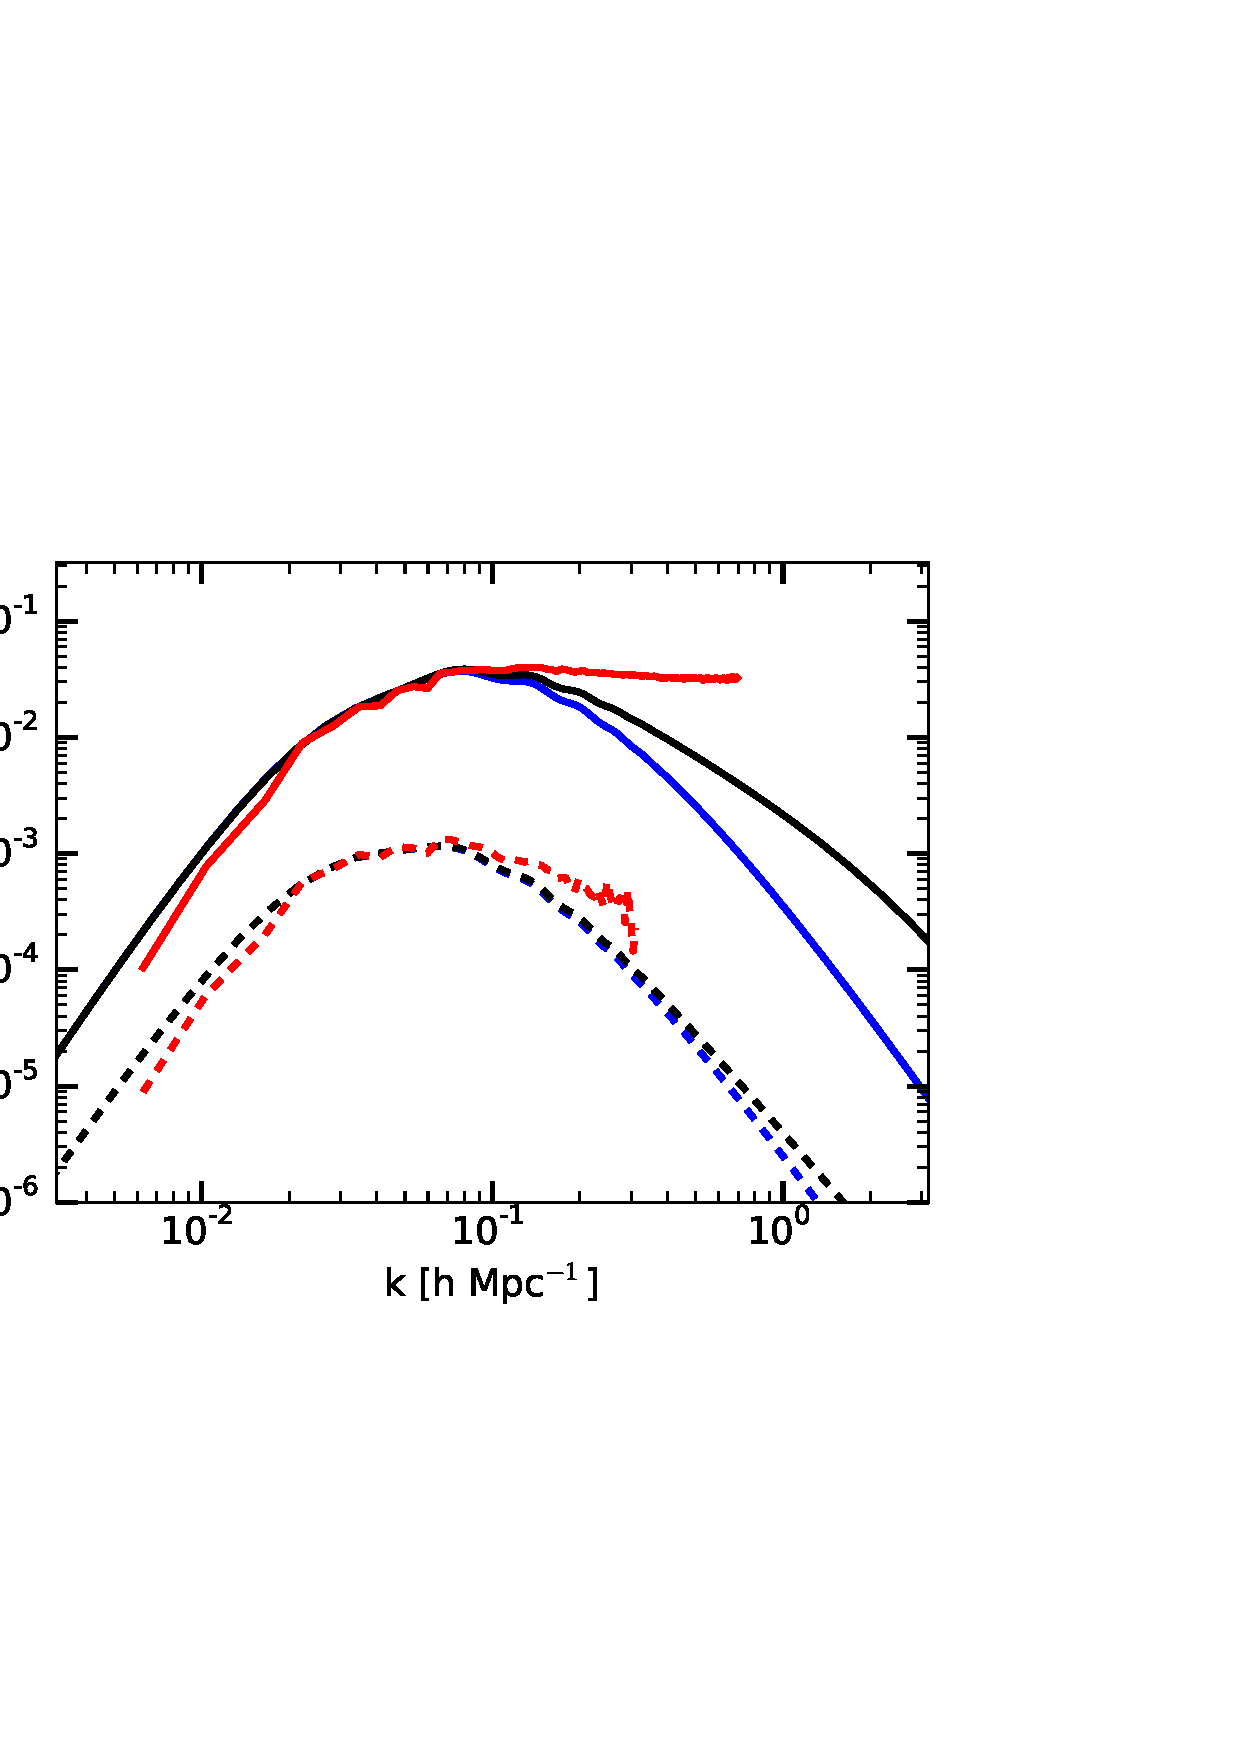
\includegraphics[width=0.495\textwidth]{Figures/density_nu.pdf}}
  \caption{
    The dimensionless CDM
    (\ref{fig:densitycdm}) and neutrino (\ref{fig:densitynu}) power
      spectra  from the
     simulations with (red lines) and without (green lines) neutrinos.  
    The CDM power spectra are shown at $z=0$ (solid lines)
     and $z=10$ (dashed lines) while the neutrino power spectra are shown
     at $z=0$ (solid lines) and $z=3$ (dashed lines).  
     The CLASS (blue) and, when they depart from the linear spectra, 
     \halofit (black) results are also shown.  
      We do not include results from the simulation without neutrinos
      at redshift $z=10$, as neutrinos are added at this redshift
      and so the two simulations are identical for $z\ge10$.  The CDM 
      power spectrum at $z=0$ from the simulation including
      neutrinos lies directly on top of the 
      CDM power spectrum from the simulation without, 
indicating that for the scales and neutrino
      mass considered in the simulations, $k<1$ h Mpc$^{-1}$ and $\textstyle\sum m_\nu
    = 0.2$, there is no appreciable effect of massive neutrinos on the
    CDM power spectrum.
%    At $z=10$, the CDM power spectrum
 %   agrees with both the linear spectrum from CLASS and the results
  %  from \halofit, which do not change the power spectrum from CLASS
   % at this redshift; non-linearities in the
  %CDM power spectrum appear negligible at this redshift.
%However, at $z=0$ the CDM power spectrum deviates
%significantly from the linear spectrum, but agrees well with the
%spectrum from \halofit, as is expected.  We see that non-linearities
%are important at $k>0.2$ h Mpc$^{-1}$ in the dark matter power spectrum.  We see
%that non-linearities in the neutrino power spectrum are important at
%$z=0$ and $z=3$, as the power spectrum deviates from the linear CLASS
%spectrum at these redshifts.  However, naively scaling the CLASS
%linear power spectrum using \halofit still underestimates the neutrino
%power at scales $k>0.2$ h Mpc$^{-1}$.
}\label{fig:density}
\end{figure*}


As discussed in Section \ref{sec:Numerics}, two 
%sets of N-body
%simulations were performed.  For each set, an 
N-body simulations were
run: one  with and one without massive neutrinos. 
%(and therefore with only CDM and
%a cosmological constant), 
%and one was run with massive neutrinos.  
In this section, the results from the simulations are
presented and compared to the CLASS results with and without scaling by \halofitns.  We use the recently
revised \halofit model \citep{takahashi12} extended to include the effects of massive
neutrinos \citep{bird12}. As we are interested in the CDM
and neutrino power spectra, not the matter power spectrum, throughout
this report we will refer to the CLASS results scaled by the
ratio of the non-linear \halofit and linear CLASS matter power spectra
as the \halofit results.
In Figure \ref{fig:density}, we
show the dimensionless CDM and neutrino power spectra,
where the dimensionless power spectrum is defined as usual:
\begin{equation}
  \Delta(k,t) = P(k,t) \frac{ k^3 }{2 \pi^2} \;.
\end{equation} 

%NEED TO CLEAN THIS UP
%When plotting the CDM density power, HALOFIT will refer
%to the CLASS results normalized using HALOFIT.  In all other, cases
%the HALOFIT is the CLASS power spectrum multiplied by the ratio
%of the non-linear (HALOFIT) and linear matter power spectra. 
% THINK WE WILL JUST CALL IT HALOFIT
%As we will see in Sections \ref{sec:Density} and \ref{sec:Velocity},
%the neutrino density and the CDM and neutrino velocity
%divergences are to first order linearly dependent on the CDM density
%perturbation. 
From Figure \ref{fig:densitycdm} we see that the CDM power
spectrum agrees with linear theory at
$z=10$.
%, indicating that at this redshift non-linear effects are
%negligible in the dark matter power spectrum for the scales resolved in
%the simulations ($k \le 1$ h
%Mpc$^{-1}$).  
At $z=0$ however, we see that non-linearities are important for $k\gsim
0.1$ h Mpc$^{-1}$.  The CDM power spectra from the
simulations with and without neutrinos are
consistent with one another and with
the \halofit power spectrum at $z=0$; this indicates that the
effect of massive neutrinos on the CDM power spectrum
is negligible for the neutrino masses considered in the simulation $\big(\sum
m_\nu = 0.2$ eV$\big)$ at $k\le 1$ h Mpc$^{-1}$.  
The numerical neutrino power spectrum deviates strongly from linear theory at wavenumbers
$k\gsim0.1$ h Mpc$^{-1}$ and as early as $z=3$, as shown in Figure \ref{fig:densitynu}.  These
results are consistent with previous numerical studies of the cosmic
neutrino background
\citep{brandbyge082,inman15} and cannot be
accounted for by simply scaling the linear result using \halofitns.

\begin{figure*}[h!]
  \centering
  \subfloat[CDM velocity divergence power\label{fig:velcdm}]{
    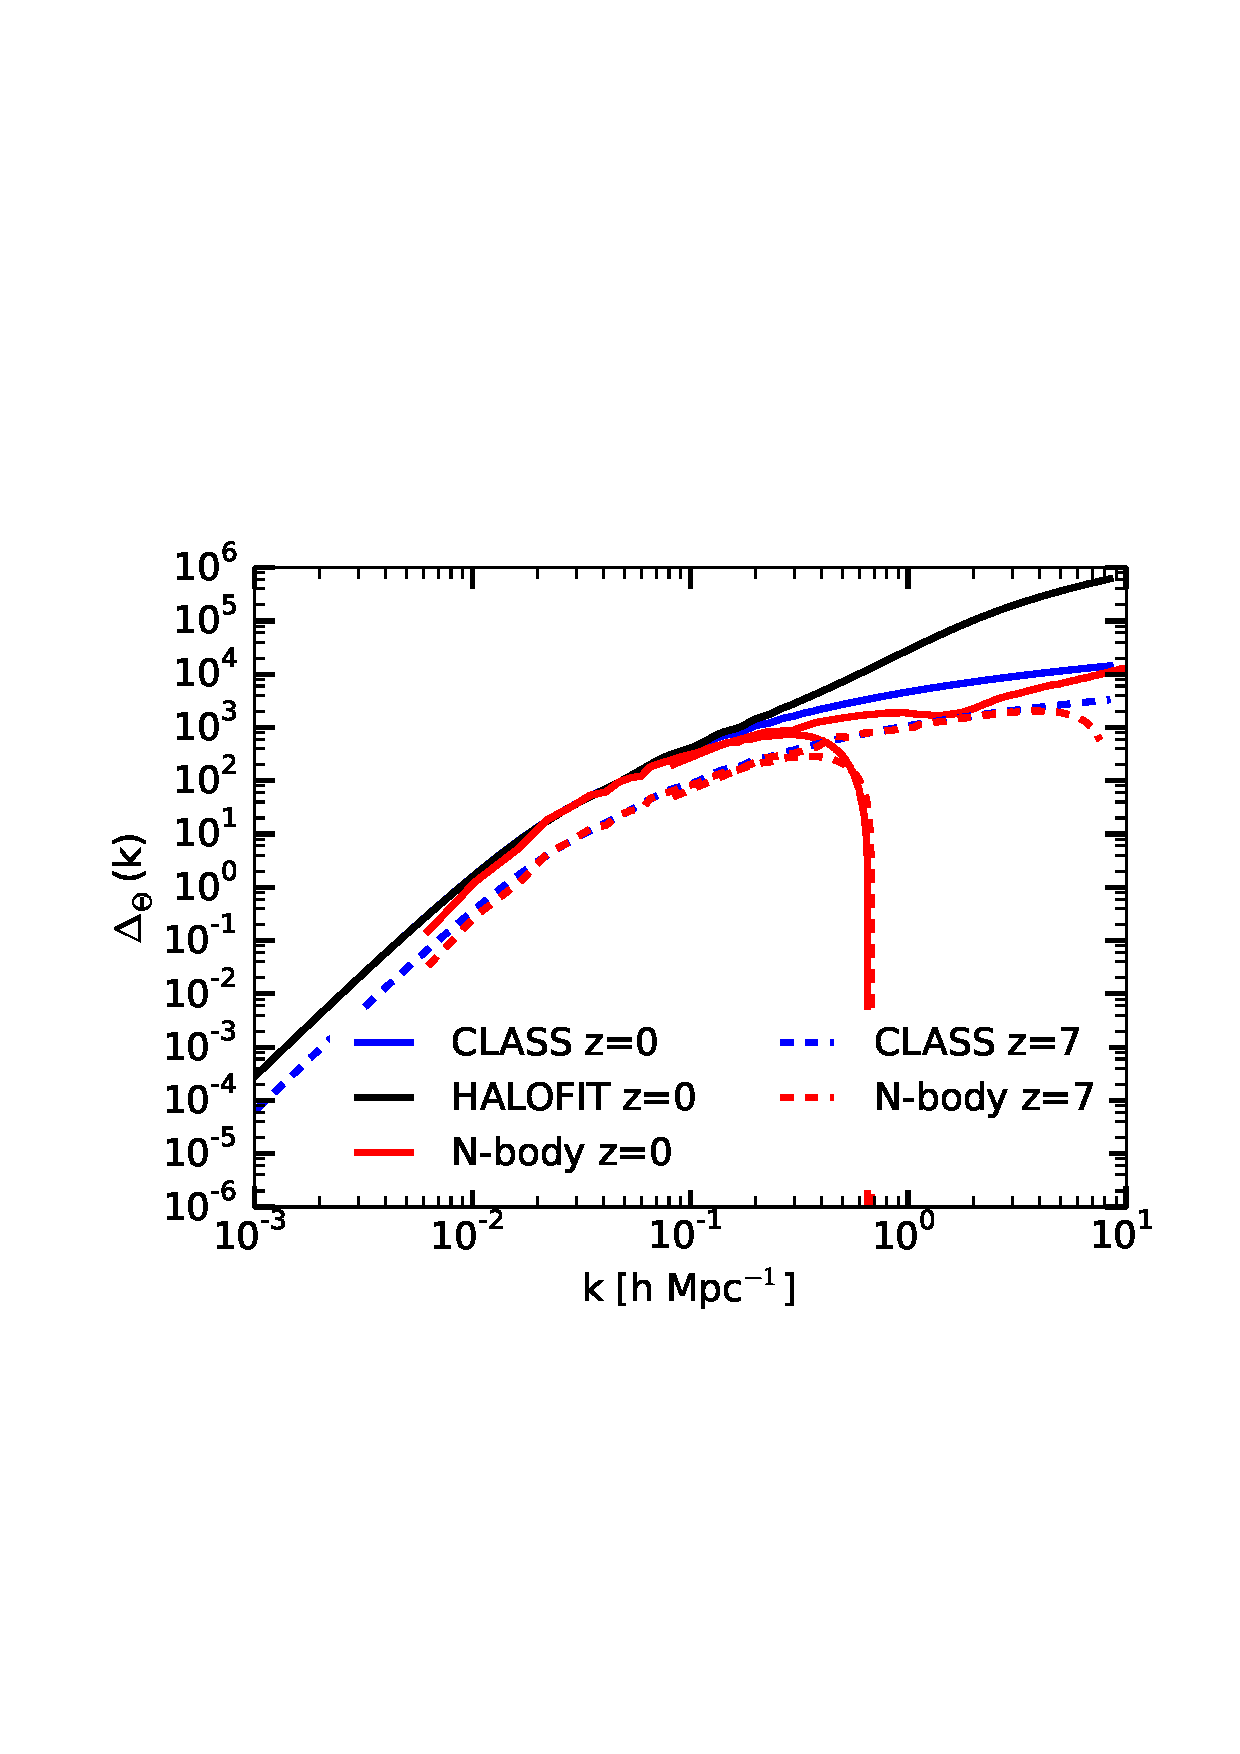
\includegraphics[width=0.495\textwidth]{Figures/vel_cdm.pdf}}
  \subfloat[Neutrino velocity divergence power\label{fig:velnu}]{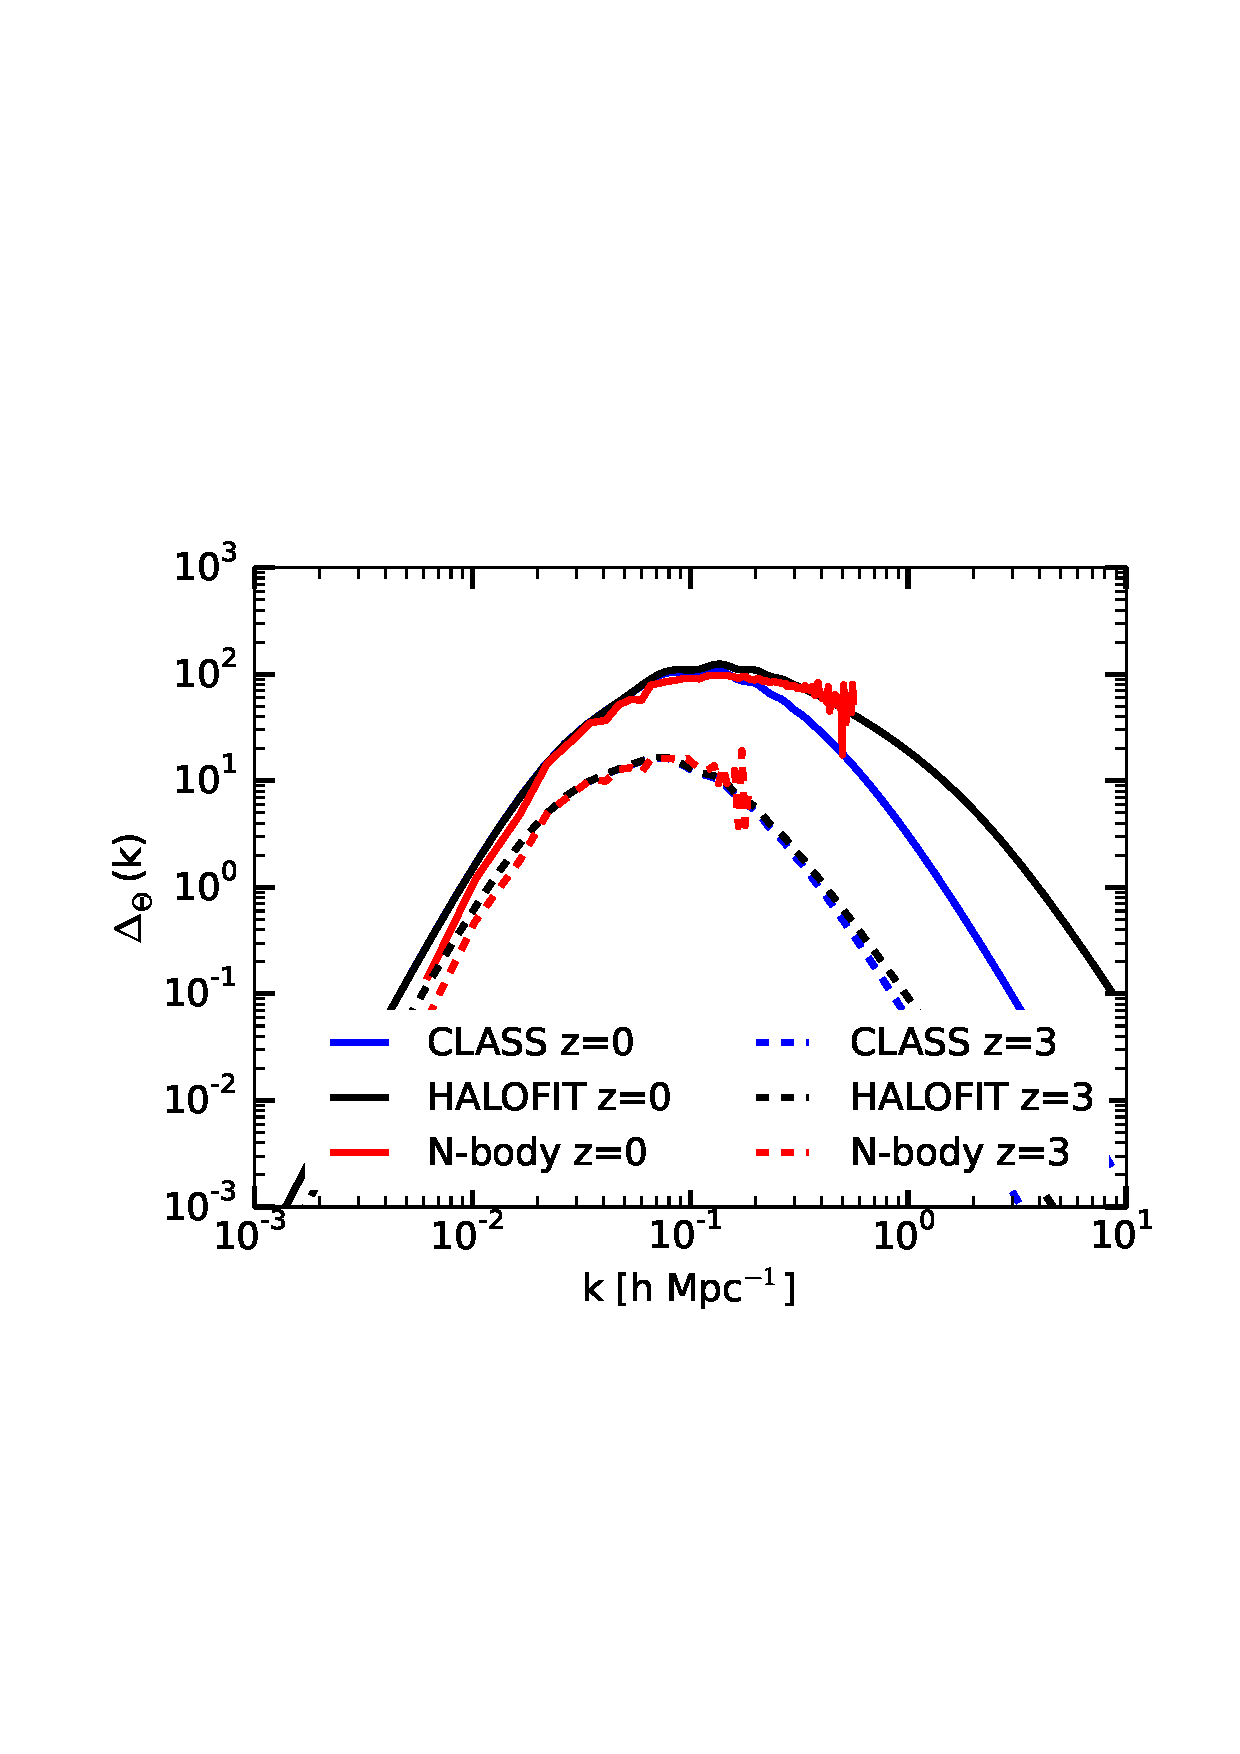
\includegraphics[width=0.495\textwidth]{Figures/vel_nu.pdf}}
  \caption{The CDM
    (\ref{fig:velcdm}) and neutrino (\ref{fig:velnu}) velocity
      divergence power
      spectra.
    %The numerical results
     % from the simulation including neutrinos (red) are plotted along
     % with the velocity divergence power spectra from CLASS (blue) and
     % \halofit (black). The CDM velocity divergence power
      %is plotted at $z=0$ (solid lines) and $z=7$ (dashed lines),
     % while the neutrino velocity divergence power is plotted at $z=0$
      %(solid lines) and $z=3$ (dashed lines).  
      The numerical CDM
      power spectra are included from two
      different simulations with different box sizes.  The
      simulation with the smaller box size is used only for comparison to
      the semi-linear results, and not for the semi-linear analysis.  
      %At $z=7$, the numerical CDM velocity
      %divergence agrees well with linear theory, but 
      At $z=0$, the
      numerical CDM velocity divergence power is
      suppressed on small scales compared to
      linear theory, opposite to what is
      expected from naively scaling the linear result using \halofitns.
      The neutrino velocity divergence power at $z=0$ is
      underestimated by linear theory, but agrees well
      with \halofit.   
}\label{fig:vel}
\end{figure*}

In Figure \ref{fig:vel}, we show the velocity divergence power
spectrum with the same normalization as the dimensionless density power spectrum:
\begin{equation}
  \Delta_\Theta(k,t) = <\Theta(\mathbf{k},t) \Theta(\mathbf{k},t)>  \frac{k^3}{2 \pi^2}  \;,
\end{equation}
where $\Theta(\mathbf{k},t) = \nabla \cdot \mathbf{v}(\mathbf{k},t)
$. 
From Figure \ref{fig:velcdm} we first notice that the numerical
simulations are unable to resolve the CDM velocity power
spectra at $k > 0.1 $ h Mpc$^{-1}$, possibly due to an
over-subtraction of noise in the calculation.
As only the CDM density fields are
necessary for the semi-linear method, this is
not a huge cause for concern; however, we plan to repeat this work
with an improved N-body simulation in the near future.
% in order to
%better the comparison with the semi-linear results.  
For comparison purposes only, we extend the numerical results using 
a second simulation with a 
box length of 75 Mpc h$^{-1}$ and a softening length of 0.625
Mpc h$^{-1}$.  
As Figure \ref{fig:velcdm} shows, at $z=7$, the numerical CDM velocity divergence power agrees with 
linear theory, but at $z=0$ 
the CDM velocity divergence power is suppressed 
compared to linear theory on scales $k\gsim0.1$ h Mpc$^{-1}$, a result also noted by \cite{inman15}.  
From Figure \ref{fig:velnu}, we see that the neutrino velocity
divergence spectrum deviates from linear theory for scales $k \gsim
0.1$ h Mpc$^{-1}$ at $z=0$ but 
is fairly well-characterized by \halofitns.  This was also noted by \cite{inman15}, who find
an $\approx 17$\% error between the two spectra at $k=1$ h
Mpc$^{-1}$. 

\begin{figure*}[h!]
  \centering
  \subfloat[$k=0.1$ h Mpc$^{-1}$\label{fig:correlators90p1}]{
    \includegraphics[width=0.495\textwidth]{Figures/correlators9_k0p1.pdf}}
  \subfloat[$k=1.0$ h Mpc$^{-1}$\label{fig:correlators91}]{
    \includegraphics[width=0.495\textwidth]{Figures/correlators9_k1.pdf}}
  \caption{The cross-correlation matrix at $k=0.1$ h Mpc$^{-1}$
      (\ref{fig:correlators90p1}) and  $k=1$ h Mpc$^{-1}$
      (\ref{fig:correlators91}) when
      the unequal-time power is calculated among twelve redshifts
      in the range $z=0$ to $z=15$.  At $k=0.1$ h Mpc$^{-1}$, the
      cross-correlation coefficients are all close to unity, indicating
      that the gravitational potential phase changes very little over
      time at this scale.
      In contrast, at $k=1$ h Mpc$^{-1}$, the cross-correlation
      coefficients fall to zero rapidly.}\label{fig:correlators}
\end{figure*}


In Figure \ref{fig:correlators}, we show the cross-correlation matrix
at $k=0.1$ h Mpc$^{-1}$ and $k=1.0$ h Mpc$^{-1}$.  The
cross-correlation coefficients were calculated among density fields at
twelve different redshifts between $z=0$ and $z=15$.
We see that at
$k=0.1$ h Mpc$^{-1}$, the cross-correlators vary slowly,
indicating that the phase of the gravitational potential remains
roughly constant over time; this is expected since this scale
remains linear today.  At $k=1.0$ h Mpc$^{-1}$, the
cross-correlation coefficients vary much more quickly and are
close to zero for the largest redshift separations.  The cross-correlation coefficient between $z=0$ and $z=0.5$, a term
two rows off-axis in the cross-correlation matrix, is 0.4 at $k=1.0$
h Mpc$^{-1}$, indicating
that we expect the semi-linear method to be
accurate for $k \lsim 1.0$ h Mpc$^{-1}$.  Because the numerical
simulations in this work
are not accurate on scales smaller than this we choose not to 
collect the density field at
additional redshifts in an attempt to push the accuracy to smaller
scales.  However, this will be necessary to test 
the semi-linear method on more non-linear scales, something we hope to accomplish
in the near future and with higher resolution numerical simulations.




%\begin{figure*}[h!]
%  \centering
%  \begin{subfigure}[t]{0.495\textwidth}
%    \centering
%    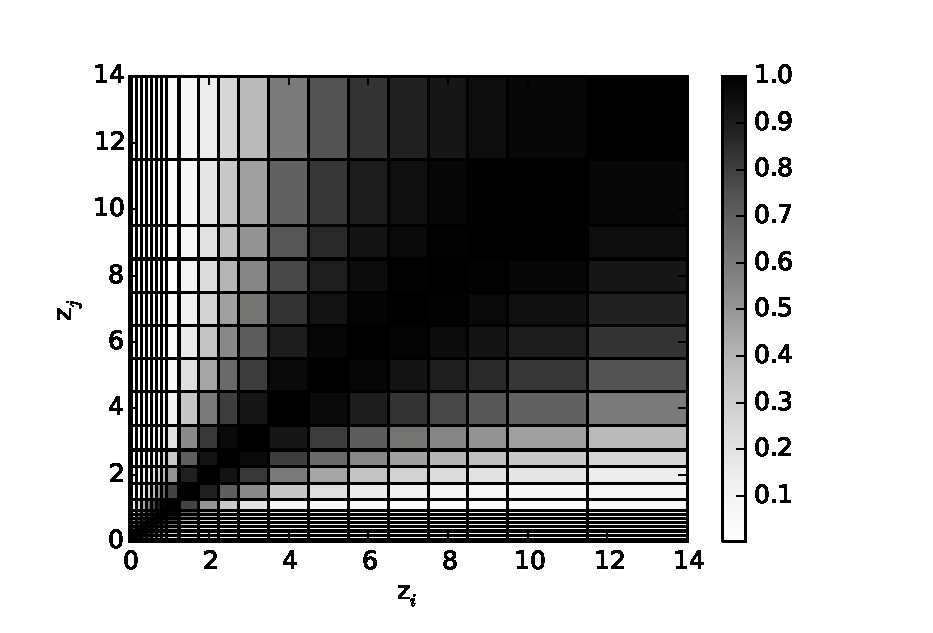
\includegraphics[width=\textwidth]{Figures/correlatorsf_k1.eps}
%    \caption{}
%    \label{fig:correlatorsf1}
%  \end{subfigure}
%  \begin{subfigure}[t]{0.495\textwidth}
%    \centering
%    \includegraphics[width=\textwidth]{Figures/correlatorsf_k1_zoom.eps}
%    \caption{}
%    \label{fig:correlatorsf0p1}
%  \end{subfigure}
%  \caption{The unequal-time cross-correlation matrix  at $k=1.0$ h
%    Mpc$^{-1}$ when
%      the unequal-time power is calculated between 22 redshifts
%      in the range $z=0$ and $z=15$.}
%\end{figure*}

\section{Density Power}
\label{sec:Density}

In the first of three parts of this analysis, we obtain the
CDM and neutrino 
density power spectra from the Euler equation \eqref{eqn:euler} and
the continuity equation \eqref{eqn:continuity}, derived in Section
\ref{sec:Fluids}, using the $w$-vectors from the numerical simulation
to measure the gravitational potential 
as described in Section \ref{sec:Methods}. We therefore require a
relation between 
the density power and the $w$-vectors.  We start by taking the gradient of the Euler equation
\eqref{eqn:euler} and differentiating the continuity equation
\eqref{eqn:continuity} with respect to time, $t$. Combining these equations, we obtain
a single equation for the density contrast in Fourier space:
%\begin{aside}
%\begin{equation}
%\begin{array}{rcl}
%  \dot{ \delta_i } + \frac{1}{a} \nabla \cdot \mathbf{u}_i &=& 0 \\[1em]
%  \dot{ \mathbf{u}_i} + \frac{ \dot{a}}{a} \mathbf{u}_i + \frac{1}{a
%  \widebar{\rho_i}} \nabla_i P &=& - \frac{1}{a} \nabla \phi_c \\[1em]
%  \ddot{ \delta_i} + \frac{1}{a} \frac{ \partial}{\partial t} ( \nabla
%  \cdot \mathbf{u}_i ) - \frac{ \dot{a}}{a^2} \nabla \cdot \mathbf{ u}
%  _i &=& 0 \\[1em]
%  \frac{ \partial}{\partial t} ( \nabla \cdot \mathbf{u}_i )  + \frac{
%  \dot{a}}{a} \nabla \cdot \mathbf{u}_i + \frac{1}{a} \nabla^2 \phi_c
%  + \frac{1}{a \widebar{\rho_c}} \nabla^2 P_i &=& 0 \\[1em]
%  \ddot{ \delta } + \frac{2 \dot{a}}{a^2} \nabla \cdot \mathbf{u}_i +
%  \frac{1}{a^2 \widebar{ \rho }} \nabla^2 P_i &=& \frac{1}{a^2} \nabla^2
%  \phi_c \\[1em]
%  \ddot{ \delta_i } - \frac{ 2 \dot{a}}{a^2} a \dot{\delta_i} + \frac{
%  1}{a^2 \widebar{\rho_i}} \nabla^2 P_i &=& \frac{1}{a^2} \nabla^2
%  \phi_c \\[1em]
%  a^2 \frac{d}{d t}( \frac{1}{a^2} \dot{\delta_i} ) + \frac{1}{a^2
%  \widebar{\rho_i}} &=& \frac{1}{a^2}\frac{3}{2} H^2 a^2 \delta_c  \\
%\end{array}
%\end{equation}
%\end{aside}
\begin{align*}\label{eqn:densitycontrast} 
  \frac{1}{a^2(t)} &\frac{d}{dt}\bigg( a^2(t) \frac{ d
  }{dt}\delta_i(\mathbf{k},t) \bigg) - \frac{\nabla^2 P_i}{a^2(t)
  \widebar{\rho_i}(t)}\\ = 
&\frac{1}{a^2(t)}\frac{3}{2} H^2(t) a^2(t) \delta_c(\mathbf{k},t) \;.\numberthis
\end{align*}
We change the coordinate $t$ to $\tau$ such that
%$\frac{d}{d\tau} = \frac{1}{a^2} \frac{d}{dt}$, 
$\frac{d}{d\tau} = a^2\frac{d}{dt}$,
%$H(\tau) = \frac{1}{a^2} H(t)$,
$H(\tau) = a^2 H(t)$,
 and Equation \eqref{eqn:densitycontrast} becomes:
\begin{equation}\label{eqn:densitycontrast2}
  \frac{d^2}{d \tau^2} \delta_i(\mathbf{k},\tau) - \frac{a^2}{\widebar{ \rho_i} }\nabla^2 P_i =
  \frac{3}{2} H^2(\tau) \delta_c(\mathbf{k},\tau)\;.
\end{equation}
For further analysis, we must distinguish between CDM and
neutrinos, as they are characterized by different
pressures in the fluid approximation.  
As discussed above, CDM can be approximated as a
pressureless fluid, while a finite pressure is necessary to account
for the significant thermal motion of neutrinos.  As mentioned in
Section \ref{sec:neutrinos}, using a finite sound speed $c_s$ such
that $c_s^2 = \frac{ \widebar{c_s}^2 }{a^2}$ accounts for this
pressure. 
%We will
%analyze these two cases in Sections \ref{sec:densitycdm} and
%\ref{sec:densitynu} below.  
%Note that any
%dependence of sound speed on time or, for example, wavenumber, may be
%considered numerically.  However, these two dependencies lend
%themselves well to a Green's function analysis. - Something to note
%in the conclusions but not here
In both of these cases, a Green's function solution to Equation
\eqref{ eqn:densitycontrast2} exists of the form
\begin{equation}
  \delta_c(\mathbf{k},\tau) = \int_{-\infty}^\tau d\tau'
  G_i(\tau,\tau') \frac{3}{2} H^2(\tau) \delta_c(\mathbf{k}, \tau'
  )\;,
\end{equation}
where $i=c,\nu$ for cold dark matter and neutrinos respectively, and
the Green's functions are 
\begin{equation}
  G_c(\tau,\tau') = \tau - \tau' 
\end{equation}
for cold dark matter and
\begin{equation}
  G_\nu(\tau,\tau') = j_0(k \widebar{c_s} (\tau - \tau' ) ) (\tau -
  \tau' ) 
\end{equation}
for neutrinos. 

This allows one to write both the cold dark matter and neutrino power
spectra in terms of the cold dark matter density perturbation as
\begin{equation}
  P_i(\tau) = < \delta_i(\tau) \delta_i^*(\tau)> = \int_{-\infty}^\tau
  d \tau' G_i(\tau,\tau') \frac{3}{2} H^2(\tau') \int_{-\infty}^\tau d
  \tau'' G_i(\tau,\tau'') \frac{3}{2} H^2(\tau'') < \delta_c(\tau')
  \delta^*_c(\tau'') > \;,
\end{equation}
or equivalently, in terms of the $w$-vectors as
\begin{equation}
  P_i(\tau) = \sum_m \bigg| \int_{-\infty}^\tau d \tau' G(\tau,\tau')
  \frac{3}{2}H^2(\tau') w^m(\tau') \bigg|^2 \; .
\end{equation}

At redshifts included in the numerical simulations, these integrals
can be calculated numerically.  However, at earlier redshifts, an
analytical expression is required.  We use the numerical potential at
redshifts $z=15$ and lower, as at these redshifts there are no
artifacts of the initial particle grid in the N-body power spectra.
It is justified to assume matter domination when calculating the early
time integrals since at $z=15$ the universe is matter dominated.
Under this assumption, the CDM density contrast scales linearly with
the scalefactor.  We will also assume that the phase of the gravitational potential
remains constant at these early times, so that we may take only the
zeroeth order w-vector to be non-zero, and we can assume that it is
equal to the density contrast:
\begin{equation}\label{eqn:matterw}
  w_M^m(k,\tau) = \begin{cases} 
    A(k) a(\tau), & \text{if } m = 0\;, \\
    0, & \text{otherwise} \;,
  \end{cases}
\end{equation}
where $A$ is a normalization factor, calculated by normalizing
Equation \eqref{eqn:matterw} to the numerical spectrum at $z=15$, and
the subscript $M$ indicates that these expressions hold during matter domination.  
%We will also use the Hubble parameter in matter domination:
%\begin{equation} 
%  H_M(t) = H_0 \sqrt{ \frac{ \Omega_M }{a^3(t) } } \;.
%\end{equation}


%\subsection{ Cold dark matter }
%\label{sec:densitycdm}
%We will treat CDM as a pressureless fluid with $\nabla
%P_c=0$ so that Equation \eqref{eqn:densitycontrast2} can be written as:
%\begin{equation}\label{eqn:densitycontrastcdm}
 % \ddot{\delta}_c(\mathbf{k},\tau) = \frac{3}{2} H^2(\tau)
 % \delta_c(\mathbf{k},\tau) \;,
%\end{equation}
%where $\dot{f}$ now indicates the derivative of $f$ with respect to
%$\tau$ and $H(\tau) = \frac{\dot{a}}{a}$.
%A Green's function solution to Equation
%\eqref{eqn:densitycontrastcdm} with $G_c(\tau,\tau') = \tau-\tau'$  exists:
%\begin{equation}\label{eqn:densitycdm}
 % \delta_c(\mathbf{k}, \tau) = \int_{-\infty}^\tau d\tau' (\tau - \tau') \frac{3}{2}
 % H^2(\tau) \delta_c(\mathbf{k},\tau')\;,
%\end{equation}
%so that we may write the density power:
%\begin{align*}\label{eqn:densitypowercdm}
 % P_c(\tau) = &< \delta_c(\tau) \delta_c^*(\tau)>\\ 
  %          =& \int_{-\infty}^\tau
 %d\tau' (\tau-\tau') \frac{3}{2} 
%H^2(\tau') \int_{-\infty}^\tau d\tau'' (\tau-\tau'') \\ &\frac{3}{2}
 % H^2(\tau'') <\delta_c(\tau') \delta_c^*(\tau'') > \;. \numberthis
%\end{align*}
%For convenience of notation, we will not explicitly indicate the
%dependence of the power spectra, $w$-vectors, and density fields on $\mathbf{k}$
%although it is implied.
%Using Equation \eqref{eqn:unequaltime} for the unequal-time CDM
% power, we can rewrite Equation
%\eqref{eqn:densitypowercdm} as:
%\begin{equation}\label{eqn:densitypowercdm2} 
%  P_c(\tau) = \sum_m \bigg| \int_{-\infty}^\tau  d\tau' (\tau-\tau')
 % \frac{3}{2} H^2(\tau') w^m(\tau') \bigg|^2 \;.
%\end{equation}
%Therefore, by performing integrals over the $w$-vectors, we
%can reconstruct the CDM density power. 

%This does seem redundant, as we require the CDM unequal-time
%power spectra in order to calculate the $w$-vectors.  
%This means that if
%the approximations that we have made up to this point were exact, and
%we calculated the eigenvectors at a sufficient number of redshift
%pairs, then the power calculated from equation
%\ref{eqn:densitypowercdm2} should be exact.  In other words,
%However, reconstructing the CDM power spectrum in this
%manner
%allows us to note the redshifts and wavenumbers for which we
%expect the approximations and the discretization that we have made in
%this analysis to hold.  It 
%allows for an analysis of the effects of
%subordinate gravitational potential modes on CDM
% and provides a verification of the accuracy of this semi-linear
%method on scales when the fluid approximation of CDM holds.

% \subsection{ Massive neutrinos }
% \label{sec:densitynu}
% As mentioned in Section \ref{sec:NuFluid}, neutrinos may be treated
% as a fluid with a finite sound speed $c_s^2
% = \frac{\widebar{c_s}^2}{a^2}$.  Recall that the sound speed is
% related to the pressure gradient via:
% \begin{equation}\label{eqn:soundspeed}
%   c_s^2 = \frac{ \partial P }{\partial \rho } = \frac{ \nabla P
%   }{\nabla \rho} = \frac{ \nabla P }{\widebar{\rho}\nabla \delta } \;,
% \end{equation}
% so that we may rewrite Equation \eqref{eqn:densitycontrast2} as:
% %\begin{equation}\label{eqn:densitycontrastnu}
% %  \frac{ d^2 }{ d \tau^2 } \delta_\nu + a^2
% %  \frac{  \widebar{c_s}^2 }{a^2} \nabla^2
% %  \delta_\nu = \frac{3}{2} H^2(\tau) \delta_c
% %\end{equation}
% %Transforming to Fourier space, we find:
% \begin{equation}\label{eqn:densitycontrastnu2}
%   \ddot{ \delta_\nu }(\mathbf{k},\tau) + k^2 \widebar{ c_s }^2 \delta_\nu(\mathbf{k},\tau) =
%   \frac{3}{2} H^2(\tau) \delta_c(\mathbf{k},\tau)\;.
% \end{equation}
% We now change coordinates to a new time $\tau$ such that
% $\frac{d}{d\tau} = \frac{a^2}{k \widebar{c_s}} \frac{d}{d t}$.  In these
% coordinates, Equation \eqref{eqn:densitycontrastnu2} reduces to:
% \begin{equation}\label{eqn:densitycontrastnu3}
%  \ddot{ \delta_\nu} + \delta_\nu = \frac{3}{2} H^2(\tau) \delta_c\;,
% \end{equation}
% where $\dot{f}$ now indicates a derivative of $f$ with respect to the new
% variable $\tau$ and $H(\tau) = \frac{\dot{a}}{a}$. 
% A Green's function solution to Equation
% \eqref{eqn:densitycontrastnu3} with
% $G_\nu(\tau,\tau')=\sin(\tau-\tau')$ exists:
% \begin{equation}\label{eqn:densitycontrastnu4}
%   \delta_\nu (\mathbf{k},\tau) = \int_{-\infty}^\tau d \tau'
%   \sin ( \tau- \tau') \frac{3}{2} H^2(\tau') \delta_c(\mathbf{k},\tau') \;.
% \end{equation}
% As we did for CDM in Section \ref{sec:densitycdm}, we can
% obtain an equation for the neutrino density power in terms of the
% $w$-vectors.  We start with:
% \begin{align*}\label{eqn:densitypowernu} 
%   P_\nu(\tau) =& < \delta_\nu(\tau) \delta_\nu^*(\tau) >\\ =&
%   \int_{-\infty}^\tau d\tau' \sin (\tau -
%     \tau')
%  \frac{3}{2}
%   H^2(\tau')  \int_{-\infty }^\tau d\tau'' \sin
%    (\tau - \tau'')\\&\frac{3}{2}
%   H^2(\tau'') <\delta_c(\tau') \delta_c^*(\tau'') > \;, \numberthis
% \end{align*}
% where once again the dependence of the power, density and
% $w$-vectors on $\mathbf{k}$ is implied.
% Using Equation \eqref{eqn:unequaltime} we can write:
% \begin{equation}\label{eqn:densitypowernu2}
%   P_\nu(\tau) = \sum_m \bigg | \int_{-\infty}^\tau d \tau' \sin
%    (\tau
%   - \tau') \frac{3}{2} H^2(\tau') w^m( \tau' ) \bigg |^2\;.
% \end{equation}
% Therefore, we can calculate the neutrino power spectrum in
% the same manner as the CDM power spectrum, but with a slightly
% different Green's function.


%\subsection{ CDM + varying sound speed }
%\label{sec:densitycdm2}
%This type of analyis is not limited to the two cases mentioned above.
%Any 

%\subsection{ The matter dominated regime}
%Since the numerical data spans a finite redshift range, 
%we must find analytic expressions for the integrals in Equations 
%\eqref{eqn:densitypowercdm2} and 
%\eqref{eqn:densitypowernu2} at high redshifts.
%We use the numerical potential at redshifts $z=15$ and
%lower, as at these
%redshifts there are no artifacts of the initial particle grid in the
%N-body power spectra.  
%, the main contribution to Equations
%\eqref{eqn:densitypowercdm2} and \eqref{eqn:densitypowernu2} from
%redshifts $z\geq 15$ is from the matter dominated era.  
%It is justified to assume matter domination when calculating the early
%time integrals since at $z=15$ the universe
%is matter dominated $\bigg(\frac{\Omega_M a^3}{\Omega_\Lambda} \approx
%1500\bigg)$.  Under this
%assumption, the CDM density contrast scales linearly with the
%scalefactor.  We assume that the phase of the
%gravitational potential remains constant at these early times, so
%that we may take the unequal-time CDM power spectrum to be:
%we will assume that only the
%primary mode of the unequal correlators contributes so that we may
%take the CDM power spectrum to be:
%\begin{equation}\label{eqn:earlytimespectrum}
%  P_{c,M}(k, \tau,\tau') = A^2(k) a(\tau) a(\tau') \;,
%\end{equation}
%where $A(k)$ is determined by
%normalizing the power spectrum to the numerical results at $z=15$ and
%we have used the subscript $M$ to indicate quantities in matter domination.  Note that we normalize at
%$z=15$ instead of $z=0$ in order to reduce the propagation of non-linear
%effects to high redshifts. 
%This gives the $w$-vectors:
%\begin{equation}\label{eqn:earlytimew}
 % w_M^m(k,\tau) = 
 % \begin{cases} 
  %  A(k) a(\tau), & \text{if } m = 0\;, \\
%    0, & \text{otherwise} \;,
%  \end{cases}
%\end{equation}
%and we will use the Hubble parameter in
%matter domination:
%\begin{equation}\label{eqn:earlytimehubble}
%  H_M(t) = H_0 \sqrt{ \frac{\Omega_M}{a^3(t)} }\;.
%\end{equation}
%Using Equations \eqref{eqn:earlytimew} and
%\eqref{eqn:earlytimehubble} we will derive analytical expressions for
%Equations \eqref{eqn:densitypowercdm2} and \eqref{eqn:densitypowernu2},
%the semi-linear CDM and neutrino power spectra respectively, in Sections
%\ref{sec:CDMmatter} and \ref{sec:NUmatter} below.

% \subsubsection{Cold dark matter}\label{sec:CDMmatter}
% For CDM, the time $\tau$ is related to the proper
% time $t$ by:
% \begin{equation}
%   \frac{ d t}{ d \tau} = a^2 \;,
% \end{equation}
% so that we can write:

% \begin{align*}
%   H_M(\tau) &= \frac{1}{a} \frac{d t}{ d \tau} \frac{da}{dt}\\
%   &= a^2(\tau) H_0 \sqrt{ \frac{\Omega_M}{a^3(\tau)}} \;. \numberthis
% \end{align*}
% This gives the following relationship between $\tau$ and the
% scalefactor, $a$:
% \begin{equation}
%   \tau = \frac{-2}{H_0 \sqrt{\Omega_M} } \frac{1}{a^{1/2} } \;.
% \end{equation}
% Using these relations, we find that the integral over early times is:
% \begin{align*}\label{eqn:cdmearly}
%   I_{c,M}(k,\tau,\tau_0) &= \int_{-\infty}^{\tau_0}d\tau' (\tau-\tau') \frac{3}{2}
%               H^2(\tau') A(k) a(\tau')\\
% %          &=& \int_{-\infty}^{\tau_0} d\tau' (\tau-\tau') \frac{3}{2}
% %      a^4(\tau') H_0^2 \frac{ \Omega_M}{a^3(\tau') } A(k) a(\tau') \\[1em]
% %          &=& \frac{3}{2} H_0^2 \Omega_M A(k) \int_{-\infty}^{\tau_0} d \tau'
% %      (\tau - \tau') \bigg( \frac{-2}{ H_0 \sqrt{ \Omega_M} } \bigg)^4
% %      \frac{1}{\tau'^4} \\[1em]
%           &= \frac{24 A(k)}{H_0^2 \Omega_M} \bigg( \frac{1}{2 \tau_0^2} - \frac{
%        \tau}{3 \tau_0^2} \bigg)\;, \numberthis
% \end{align*}
% where $\tau$ is the time at which the power is being calculated and
% $\tau_0$ is the earliest time at which we use the numerical potential
% in the integration.  The subscript $M$ indicates that the integral is
% calculated under the assumption of matter domination.  In
% order to calculate the fully analytic result, we simply set
% $\tau_0 = \tau$:
% \begin{align*}
%   P_{c,M}(k,\tau) &= \bigg|\int_{-\infty}^{\tau} d\tau' (\tau - \tau')\frac{3}{2} H^2(\tau') A(k)
%   a(\tau')\bigg|^2 \\
% %&=& \bigg|A(k) \frac{ 4 }{ H_0^2 \Omega_m \tau^2}\bigg|^2\\[1em]
% & = A^2(k)
%     a^2(\tau) \;. \numberthis
% \end{align*}
% Therefore, Equation \eqref{eqn:cdmearly} reduces to the
% correct expression for the CDM power spectrum in matter
% domination. 

% \subsubsection{Massive neutrinos}\label{sec:NUmatter}
% For neutrinos, the method is similar.  For the time coordinate $\tau$ in Equation
% \eqref{eqn:densitypowernu2}, we find:
% \begin{align*}
%   H_M(\tau) &= \frac{1}{a} \frac{ d}{d \tau} \frac{da}{dt} \\
%   & =  \frac{a^2(\tau)}{k\widebar{c_s}} H_0 \sqrt{ \frac{\Omega_m}{a^3(\tau)}} \numberthis
% \end{align*}
% and 
% \begin{equation}
%   \tau = \frac{ -2 k \widebar{c_s}}{ H_0 \sqrt{ \Omega_M } }
%   \frac{1}{a^{1/2}} \;. 
% \end{equation}
% Therefore, the integral over early times is:
% \begin{align*}
%   I_{\nu,M}(k,\tau, \tau_0) =& \int_{-\infty}^{\tau_0} d \tau' \sin( \tau - \tau' ) \frac{3}{2}
%   H^2(\tau') A(k) a(\tau') \\
% %            &=& \int_{-\infty}^{\tau_0} d \tau' \sin(\tau
% %                            - \tau' ) \frac{3}{2} \frac{a^4(\tau')}{k^2
% %                            \widebar{c_s}^2 } H_0^2 \frac{
% %                            \Omega_M}{a^3(\tau') } A a(\tau') \\[1em]
% %  &=& \frac{3}{2} \frac{H_0^2 \Omega_M}{k \widebar{c_s}} A(k)
% %      \int_{-\infty}^{\tau_0} d \tau' sin( \tau - \tau' ) \bigg(
% %      \frac{-2 k \widebar{ c_s } }{ H_0 \sqrt{\Omega_M} } \bigg)^4
% %      \frac{1}{\tau'^4}  \\[1em]
%    =& \frac{24 k^2 \widebar{c_s}^2 }{ H_0^2 \Omega_M} A(k)
%         \frac{1}{12 \tau_0^3} (2 \tau_0
%         \cos(\tau-\tau_0)+ \\
%   &2 \tau_0^3
%         \cos(\tau) \text{Ci}(-\tau_0)+ \\
% &
%   \pi
%         \tau_0^3 \sin(\tau)+2
%         \left(-2+\tau_0^2\right)
%         \sin(\tau-\tau_0)+ \\
% &
%                            2 \tau_0^3
%         \sin(\tau) \text{Si}(\tau_0) ) \;, \numberthis
% \end{align*}
% where Si and Ci are the sine integral and cosine integral functions,
% \begin{equation}
%   \text{Si}(x) = \int_0^x \frac{\sin(y)}{y} dy 
% \end{equation}
% and
% \begin{equation}
%   \text{Ci}(x) = -\int_x^\infty \frac{\cos(y)}{y} dy
% \end{equation}
% respectively.
% Once again, we can obtain a purely analytic
% expression for the neutrino power spectrum in the matter dominated
% regime by setting $\tau_0=\tau$.  In this case, the expression above
% reduces to:
% \begin{align*}
% P_{\nu,M}(k,\tau) =& \bigg|\int_{-\infty}^{\tau} d \tau' \sin(\tau-\tau') \frac{3}{2} H^2{\tau'}
% A(k) a(\tau' ) \bigg|^2 \\
% =& \bigg| \frac{24 k^2 \widebar{c_s}^2 A(k)}{ H_0^2 \Omega_M}
% \frac{1}{12} \bigg( \frac{2}{\tau^2} + \\
% &2 \cos( \tau ) \text{CI}( -
% \tau ) + \sin( \tau ) \big( \pi + 2 \text{SI}(\tau) \big) \bigg)
%     \bigg|^2 \;. \numberthis
% \end{align*}
 
\subsection{ Density power results}
We now have all of the information required to calculate the CDM
and neutrino density powers.  We will break down Equations
\eqref{eqn:densitypowercdm2} and \eqref{eqn:densitypowernu2} as follows:
\begin{align*}\label{eqn:densbymode}
  P_i(k,\tau) =& \bigg| \int_{-\infty}^{\tau_0} d\tau' G_i(\tau,\tau')
                 \frac{3}{2} H^2_M(\tau') w^0_M(k,\tau') +\\
  &\int_{\tau_0}^{\tau} d \tau'
  G_i(\tau-\tau') \frac{3}{2} H^2(\tau') w^0(k,\tau') \bigg |^2 +\\
&  \sum_{m=1}^{m_{max}} \bigg| \int_{\tau_0}^\tau d\tau' G_i(\tau -
  \tau' ) \frac{3}{2} H^2 (\tau') w^m(k,\tau') \bigg |^2 \;, \numberthis
\end{align*}
where $\tau_0$ is the time when we begin retaining the cold dark
matter density fields from the numerical simulations.
The matter domination integral is calculated analytically, while the
remaining integrals are calculated numerically using a trapezoidal
integration method after interpolating the $w$-vectors over redshift.

%\subsection{ Results of the Reconstruction}
%\begin{wrapfigure}{l}{0.5\linewidth}
\begin{figure*}[h!]
  \centering
    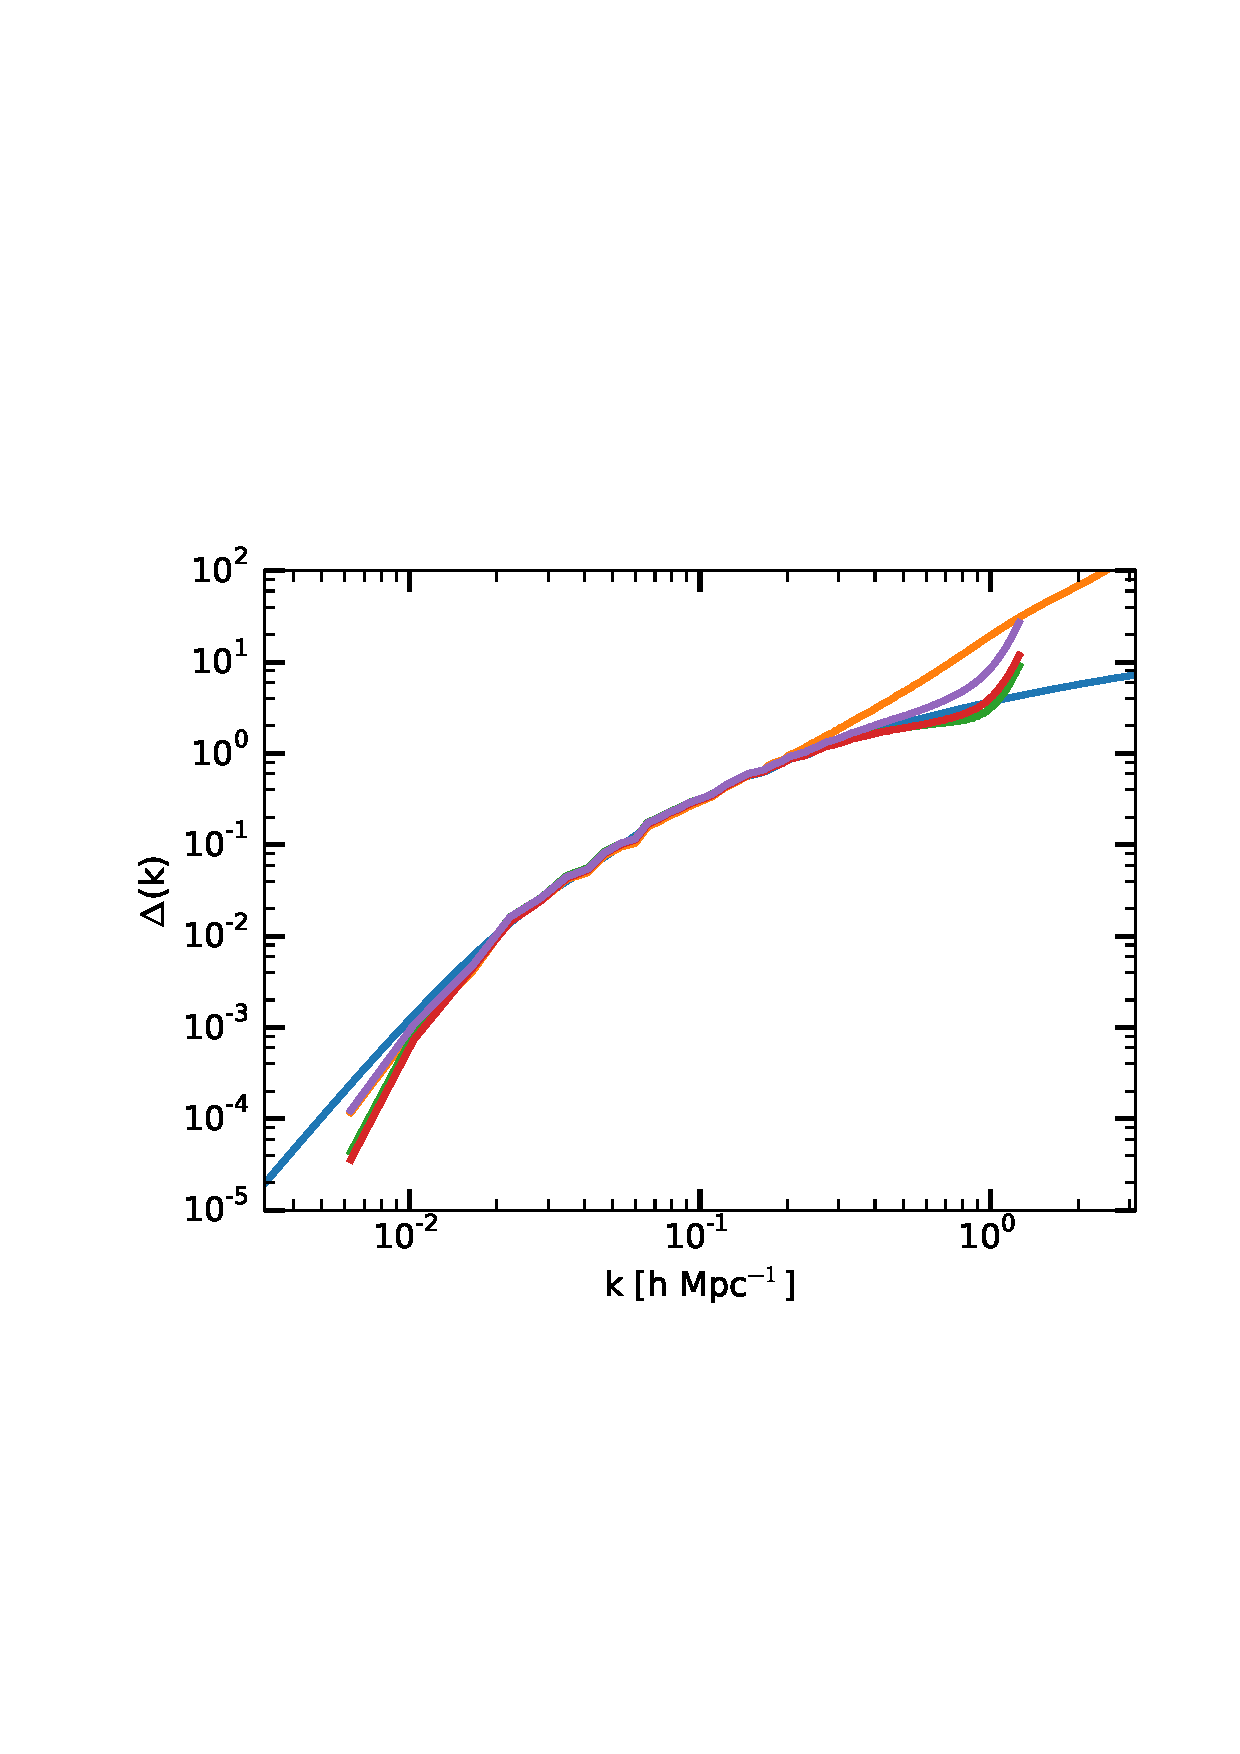
\includegraphics[width=0.495\textwidth]{Figures/density_cdm_0.pdf}
    \caption{The semi-linear CDM density power spectrum at $z=0$ along with the
      spectra from the N-body simulation (solid
      violet),
      CLASS (dotted blue), and \halofit (dotted teal).  
The semi-linear power spectrum is calculated with only the primary
eigenmode from the decomposition of the cross-correlation matrix
(dashed green), with 12 modes (solid orange), and under the assumption
that the gravitational potential remains in phase over time
(dot-dashed red).
      The semi-linear power spectra are not a significant improvement
      upon linear theory.  
%This is not unexpected as the fluid treatment of neutrinos by
%definition breaks down when the CDM power spectrum
%becomes non-linear.
}
    \label{fig:delta_cdm_rec}
\end{figure*}
%\end{wrapfigure}

In Figure \ref{fig:delta_cdm_rec} we compare the semi-linear CDM
 power spectrum at redshift $z=0$ to the CLASS, \halofitns, and
numerical power spectra. We find that the semi-linear method does not improve
significantly on linear theory.  This is not surprising, as a linear
treatment of CDM is expected to break down on small scales and
at late times when CDM clusters significantly.  
%Even though this method uses the fully non-linear
%potential, when this potential deviates from the linear potential the
%fluid approximation is not applicable, so we are unable to improve
%on linear theory.  
We also note that the semi-linear power is highest when phase changes 
in the gravitational potential are ignored.  
This follows from the Cauchy-Schwarz inequality, which
states that the cross-power between two fields is largest when they
are in phase.

\begin{figure*}[h!]
  \centering
  \subfloat[$\sum m_\nu = 0.2$ eV\label{fig:delta_nu0p2_rec}]{
    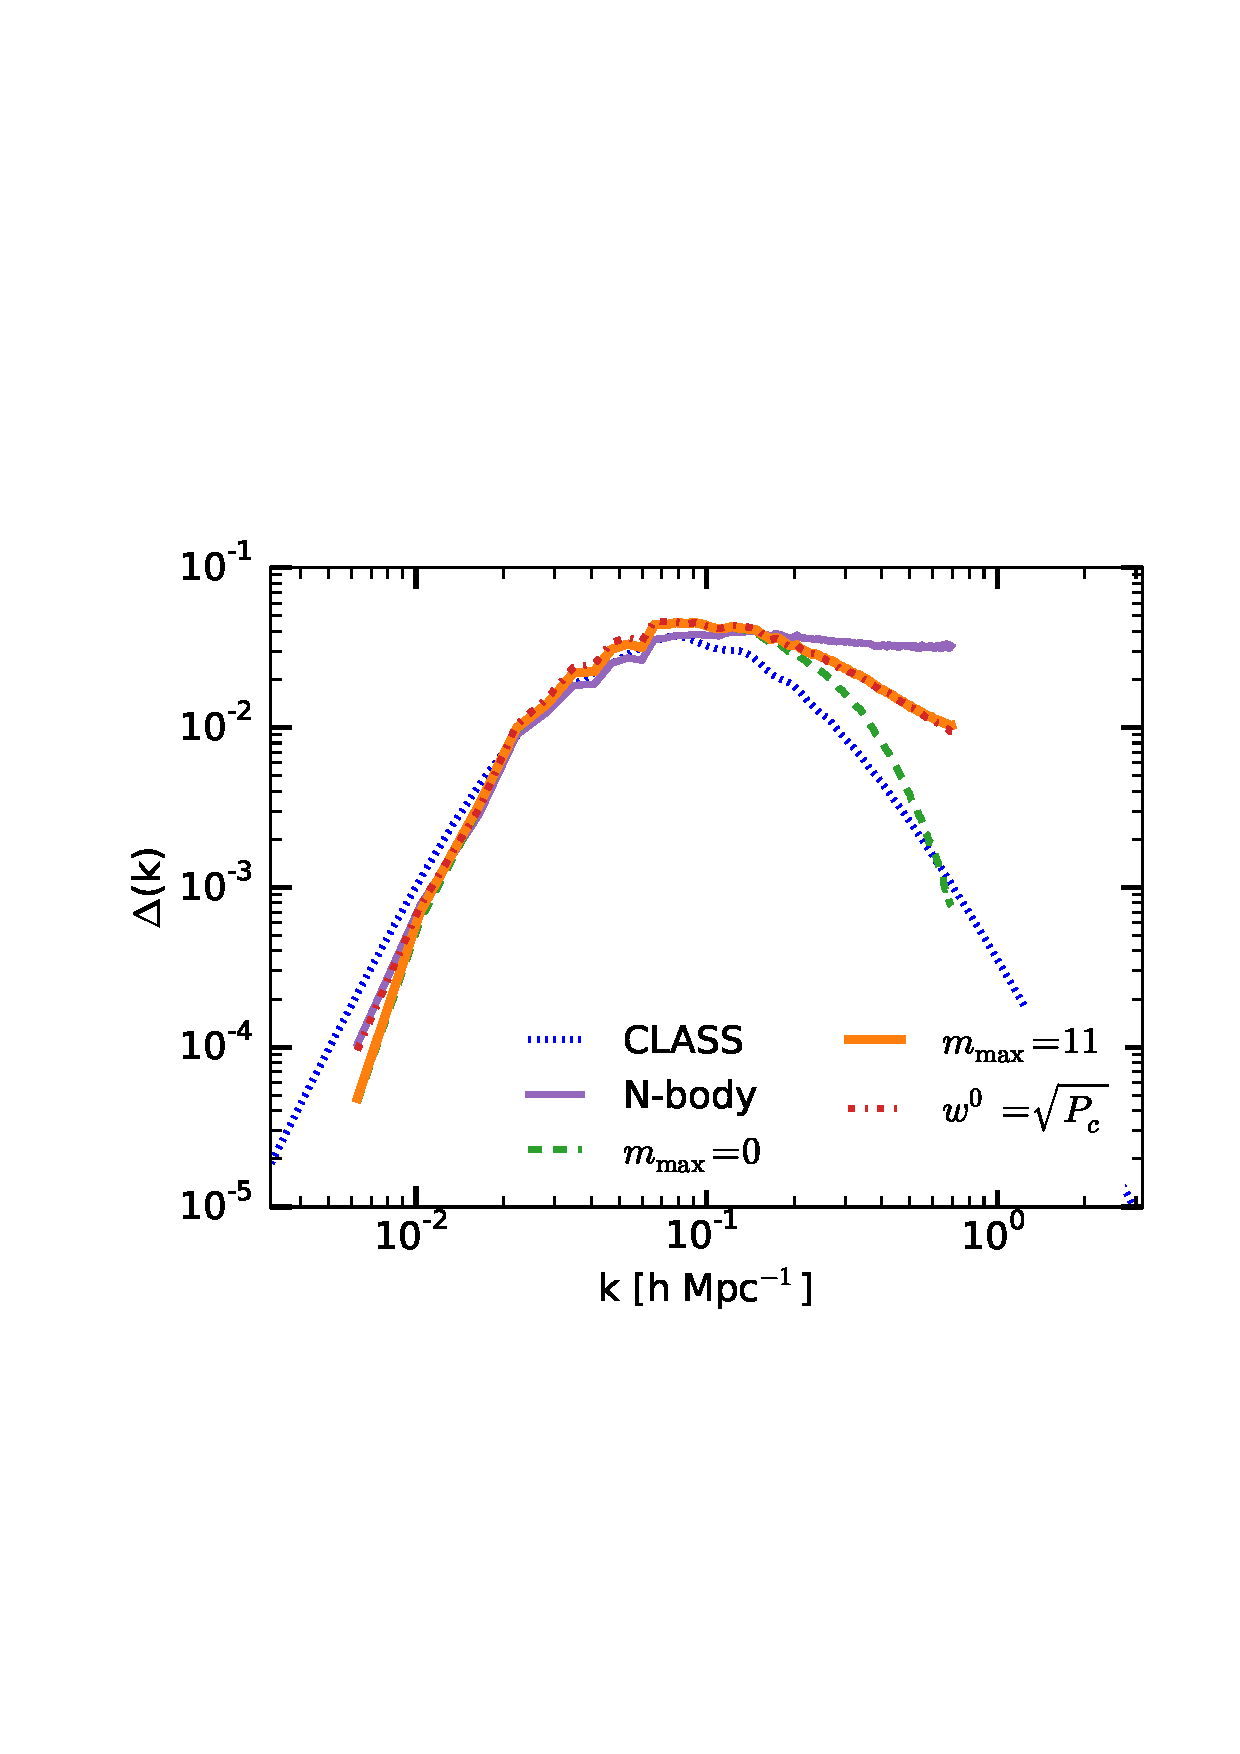
\includegraphics[width=0.495\textwidth]{Figures/density_nu0p2_0_pres.pdf}}
  \subfloat[$\sum m_\nu = 0.1$ eV\label{fig:delta_nu0p05_rec}]{
    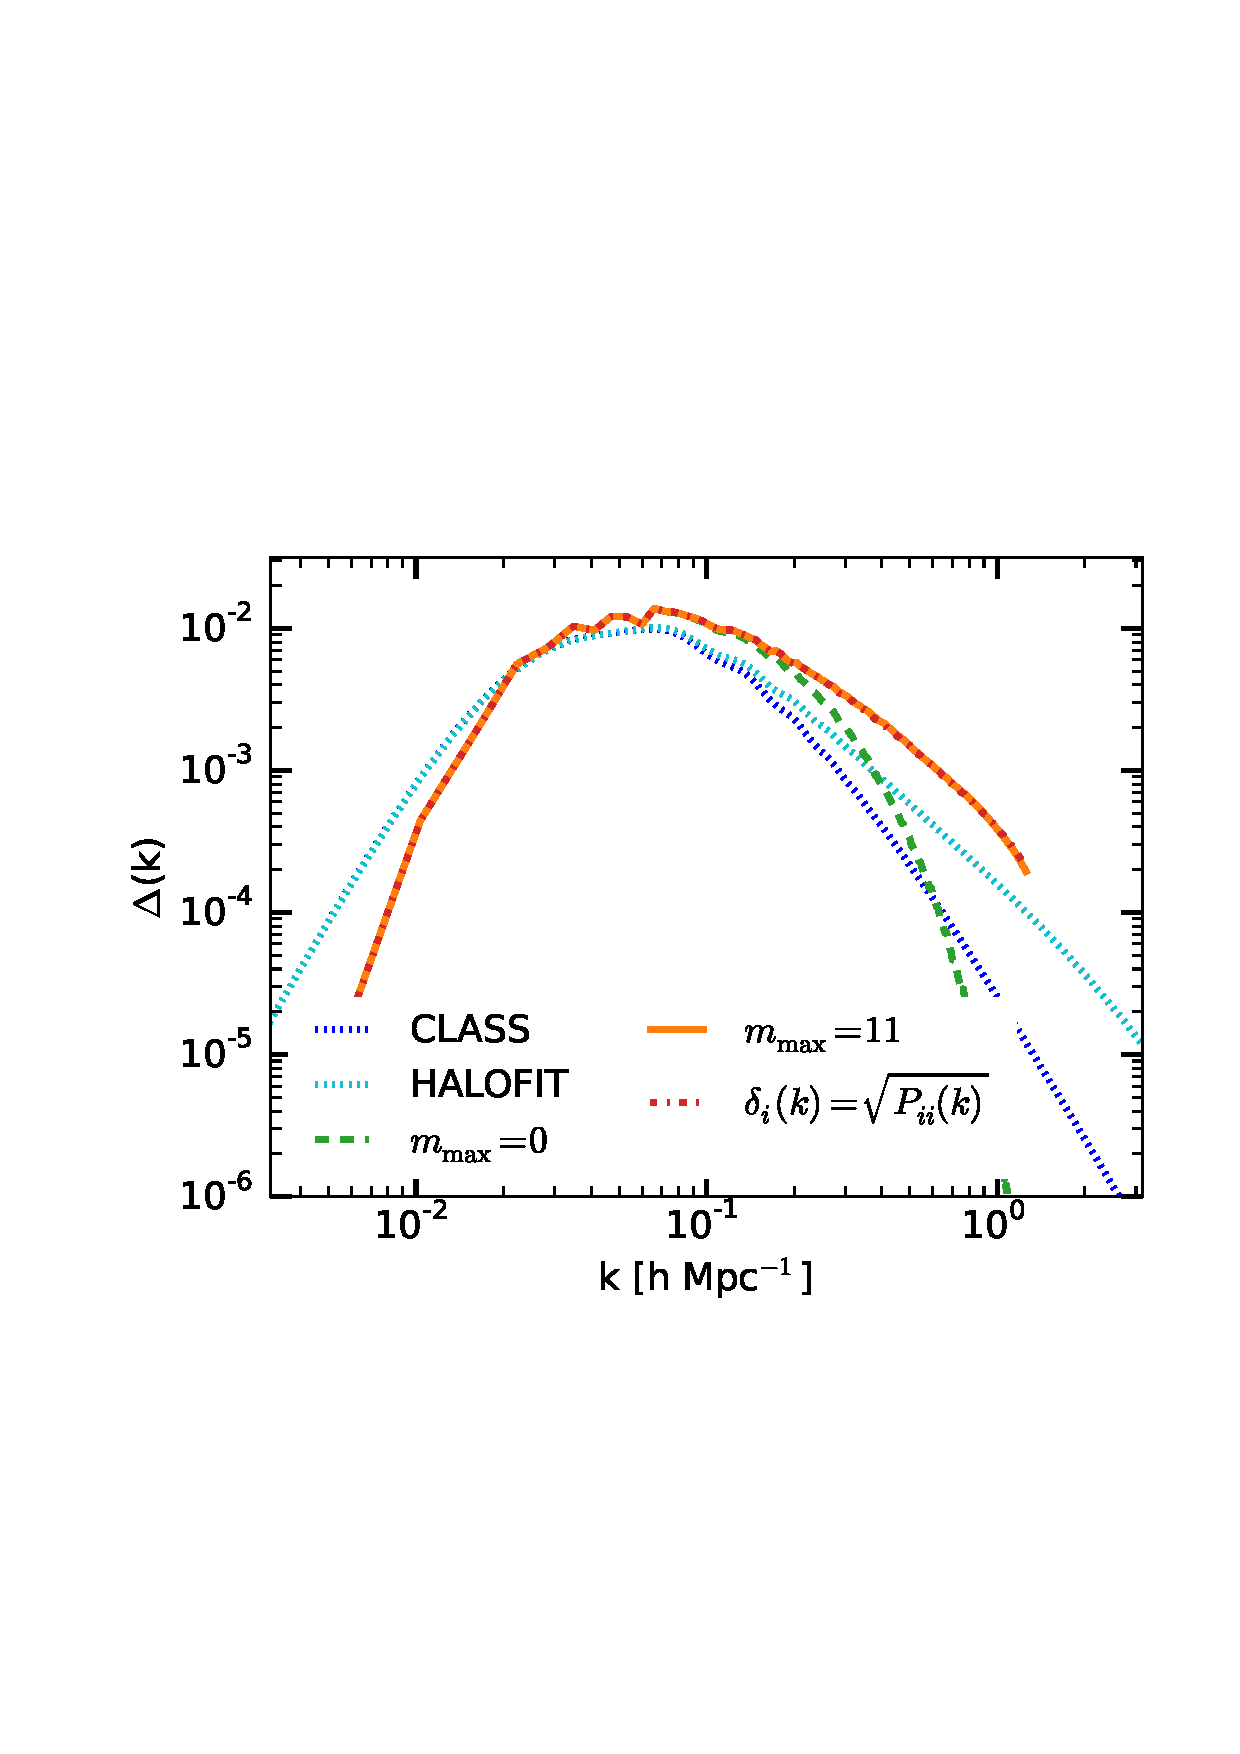
\includegraphics[width=0.495\textwidth]{Figures/density_nu_0p1.pdf}}
  \caption{The semi-linear neutrino density power spectra at $z=0$ for
      $\textstyle\sum m_\nu =0.2$ eV (\ref{fig:delta_nu0p2_rec}) and $\textstyle\sum
      m_\nu = 0.1$ eV (\ref{fig:delta_nu0p05_rec}) compared to
      CLASS (dotted blue), \halofit (dotted teal), and the N-body simulation (solid purple).  The semi-linear power spectrum is calculated with only the primary
eigenmode from the decomposition of the cross-correlation matrix
(dashed green), with 12 modes (solid orange), and under the assumption
that the gravitational potential remains in phase over time
(dot-dashed red). As no
      simulation was performed with $\textstyle\sum m_\nu = 0.1$ eV, we have not
      included numerical results in Figure
      \ref{fig:delta_nu0p05_rec}.  The
      semi-linear method improves upon linear theory and has a higher
      power than the \halofit spectrum on small scales, but does not
      accurately reproduce the neutrino density power spectrum at
      $k\gsim0.2$ h Mpc$^{-1}$. When many modes are included, the
      results match those obtained by neglecting the changing phase of
      the gravitational potential. }
    \label{fig:delta_nu_rec}
\end{figure*}

In Figure \ref{fig:delta_nu_rec}, we show the semi-linear
 neutrino power spectrum for both $\sum m_\nu =
0.2$ eV (Figure \ref{fig:delta_nu0p2_rec}) and $\sum m_\nu = 0.1$ eV
(Figure \ref{fig:delta_nu0p05_rec}).  In contrast to the CDM
 results, the semi-linear neutrino power
spectra are an improvement on both linear theory and \halofit and
agree with the numerical power spectrum for $k \lsim 0.2$ h
Mpc$^{-1}$, even when only the
primary $w$-vector is included in the calculation.  
We find that increasing the number of $w$-vectors included causes the
small scale power to increase, improving the error at
small scales; however it does not increase the range of wavenumbers at
which this method provides an accurate representation of the N-body
power spectrum. We also see that when we include many modes the
 results agree well with those obtained when the phase of
the gravitational potential is assumed to be unchanging.  
%SHOULD EXPAND ON THIS

\section{Velocity Power}
\label{sec:Velocity}

The method described in this report can be used to
calculate many fluid properties via the fluid equations.  
In this section, we discuss using this method to obtain 
the velocity divergence power
spectrum.  From the continuity equation
\eqref{eqn:continuity}, we can write the velocity divergence, $\Theta_i(\mathbf{k},t)$, in terms
of the density perturbation:
\begin{equation}\label{eqn:veldivg}
  \Theta_i(\mathbf{k},t) = \nabla \cdot \mathbf{u}_i(\mathbf{k},t) = - a \frac{ \partial \delta_i(\mathbf{k},t)}{\partial
    t} = -a \frac{ \partial \tau}{ \partial t } \frac{ \partial
    \delta_i(\mathbf{k},t) }{ \partial \tau}\;.
\end{equation} 
Therefore by using Equations \eqref{eqn:densitycdm} and \eqref{eqn:densitycontrastnu4} for the
CDM and neutrino density perturbations, we can calculate the velocity
divergence power for both species:
\begin{equation}\label{eqn:velocitydivg}
  \Theta_i(\mathbf{k},t) = \frac{1}{a^2(\tau)} \sum_m \bigg|
  \int_{-\infty}^\tau d \tau' G_{v,i}(\tau,\tau') \frac{3}{2} H^2(\tau') w^m(k,\tau')
  \bigg |^2
\end{equation}
where 
\begin{equation}
  G_{\Theta_\nu} = \cos(k \widebar{c_s} (\tau - \tau') )
\end{equation}
for neutrinos and
\begin{equation}
G_{\Theta_c} = 1 
\end{equation} 
for cold dark matter.
In Fourier space, the velocity and the velocity divergence are closely
related by $ \nabla \cdot \mathbf{u} = i \mathbf{k} \cdot \mathbf{u}
$.  Therefore, we can calculate the power of the velocity magnitude
from the velocity divergence power.

Once again, at early times we require an expression for the integrals
in Equation \eqref{eqn:velocitydivg}, which we again calculate under the
assumption of matter domination.


%\subsection{ Cold dark matter }\label{sec:velcdm}

% Using Equation \eqref{eqn:densitycdm} for the CDM density perturbation, we can expand
% Equation \eqref{eqn:veldivg} as follows:
% \begin{align*}\label{eqn:veldivgcdm}
%   \Theta_c(\mathbf{k}, \tau) & = \nabla \cdot
%                                    \mathbf{u}_c(\mathbf{k},\tau) \\
% &=-a(\tau) \frac{ \partial \tau }{ \partial t }
%                                 \frac{ \partial \delta_c (\mathbf{k},\tau)}{\partial
%                                 \tau} \\
%   &= -\frac{1}{a(\tau)} \frac{d}{d\tau} \int_{-\infty}^{\tau} d\tau' (\tau
%       - \tau') \frac{3}{2} H^2(\tau') \delta_c(\mathbf{k},\tau') \\
%  &= - \frac{1}{a(\tau)} \int_{-\infty}^{\tau} d\tau' \frac{3}{2} H^2(\tau')
%      \delta_c(\mathbf{k},\tau')\;. \numberthis
% \end{align*} 
% We write the velocity divergence power in terms of the $w$-vectors as we did for the density power:
% \begin{align*} \label{eqn:veldivgcdm2}
%   P_{\Theta_c}( k,\tau ) =& < \Theta_c(\mathbf{k},\tau) \Theta_c^*(\mathbf{k},\tau)>  \\
%   =& \frac{1}{a^2(\tau)} \int_{-\infty}^{\tau} d\tau' \frac{3}{2}
%       H^2(\tau')\\
% & \int_{-\infty}^{\tau} d\tau'' \frac{3}{2} H^2(\tau'')
%       < \delta_c(\mathbf{k},\tau') \delta_c^*(\mathbf{k},\tau'') >\\
%   =& \frac{1}{a^2(\tau)} \sum_{m} \bigg| \int_{-\infty}^{\tau} d\tau'
%       \frac{3}{2} H^2(\tau') w^m(k, \tau') \bigg|^2\;. \numberthis
% \end{align*}
% %Using Equation \eqref{eqn:veldivgcdm2} we can calculate the velocity divergence power
% %from the $w$-vectors.  
% Note that integral in Equation
% \eqref{eqn:veldivgcdm2} is essentially a Green's function integral with
% a Green's function $G_{\Theta_c}(\tau, \tau' ) = 1$. 

% %Once again, this method is slightly redundant, as we have the
% %numerical CDM spectrum from the N-body simulation and can
% %attain the velocity divergence spectrum by taking numerical
% %derivatives of the spectrum.  However, especially as the continuity
% %equation contains fewer approximations than the Euler equation, this
% %once again allows us to determine how well and up until which
% %wavenumber the approximations and discretization used in this work
% %are valid.

% We need expressions for evaluating
% the integral in Equation \eqref{eqn:veldivgcdm2} at early times, when we
% do not have numerical data from the simulation.  As in Section
% \ref{sec:Density}, we will calculate this integral at early times under 
% the assumption of matter domination using Equations \eqref{eqn:earlytimew} and \eqref{eqn:earlytimehubble} for the
% $w$-vectors and Hubble factor respectively, resulting in:
% \begin{align*}\label{eqn:intveldivgcdmmatter}
%   I_{{\Theta_c},M}(k,\tau,\tau_0) %&=&\int_{-\infty}^{\tau_0} d\tau' \frac{3}{2} H^2(\tau')
% %               w^0(\tau',k) \\[1em]
%            &=
%   \int_{-\infty}^{\tau_0} d\tau' \frac{3}{2} a(\tau')^4 H_0^2 \Omega_M
%   A(k) a(\tau') \\
% %  &=& \frac{3}{2} H_0^2 \Omega_M A(k) \int_{-\infty}^{\tau_0} d\tau' \bigg(
% %      \frac{ -2 }{ H_0 \sqrt{\Omega_M}} \bigg)^4 \frac{1}{\tau'^4}\\[1em]
%   &= \frac{-1}{3} \frac{ 24 A(k) }{ H_0^2 \Omega_M}
%     \frac{1}{\tau_0^3}\;. \numberthis
% \end{align*}
% To obtain a purely analytic expression for the CDM velocity
% divergence power in the matter dominated era, we set $\tau_0 =
% \tau$ in Equation \eqref{eqn:intveldivgcdmmatter}:
% \begin{equation}\label{eqn:intveldivgcdmmatter2}
%  I_{{\Theta_c},M}(k,\tau,\tau)  = 
%                                                                      -\frac{8
%                                                                      A(k)}{H_0^2
%                                                                      \Omega_M}
%                                                                      \frac{1}{\tau^3} \;.
% \end{equation}
% Substituting this into the Equation \eqref{eqn:veldivgcdm2} we obtain:
% \begin{equation}\label{veldivgcdmmatter}
%   P_{\Theta_c,M}(k,\tau) = \frac{1}{a^2(\tau)} \bigg| \frac{8
%     A(k)}{H_0^2 \Omega_M} \frac{1}{\tau^3} \bigg|^2 \;.
% \end{equation}
% %We expect the semi-analytical $P_{\Theta_c}(\tau,k)$ to match this
% %expression closely at low wavenumber and high redshift.

% %\subsection{ Massive neutrinos }\label{sec:velnu}
% Along the same lines as in Section \ref{sec:velcdm}, 
%  we can
%  expand Equation \eqref{eqn:veldivg} using Equation
%  \eqref{eqn:densitycontrastnu4} for the neutrino density perturbation as follows:
% \begin{align*}\label{eqn:veldivgnu}
%   \Theta_\nu( \mathbf{k},\tau) =& \nabla \cdot
%                                   \mathbf{u}_\nu(\mathbf{k},\tau) \\
%  =& -a(\tau) \frac{ \partial \tau}{\partial t}
%                                   \frac{ \partial \delta_c(\mathbf{k},\tau)
%                                   }{\partial \tau} \\
%   =& - \frac{k \widebar{c_s}}{a(\tau)} \frac{d}{d \tau}
%       \int_{-\infty}^{\tau} d\tau' \sin(\tau - \tau') \frac{3}{2}
%       H^2(\tau') \delta_c(\mathbf{k},\tau') \\
%   =& - \frac{ k \widebar{c_s}}{a(\tau)} \int_{-\infty}^{\tau} d\tau'
%       \cos(\tau - \tau') \frac{3}{2} H^2(\tau')
%     \delta_c(\mathbf{k},\tau') \;. \numberthis
% \end{align*}
% We can now express the neutrino velocity divergence power in terms of
% the $w$-vectors:
% \begin{align*}\label{eqn:veldivgnu2}
%   P_{\Theta_\nu}(k,\tau) =& < \Theta_\nu(\mathbf{k},\tau) \Theta^*_\nu(\mathbf{k},\tau) >  \\
%   =& \bigg( \frac{k \widebar{c_s} }{a(\tau)} \bigg)^2 \int_{-\infty}^\tau d
%       \tau' \cos( \tau-\tau') \frac{3}{2} H^2(\tau')
%       \\ &\int_{-\infty}^\tau d\tau'' \cos( \tau-\tau'') \frac{3}{2} H^2
%       (\tau'') <\delta_c(\mathbf{k},\tau')\delta^*_c(\mathbf{k},\tau'')>\\
%   =& \bigg(\frac{k \widebar{c_s}}{a(\tau)} \bigg)^2 \sum_m \bigg|
%       \int_{-\infty}^\tau d\tau' \cos( \tau-\tau') \\ 
%                           &\frac{3}{2}
%       H^2(\tau') w^m(k, \tau') \bigg|^2 \;. \numberthis
% \end{align*}
% This is analogous to a Green's function solution with
% $G_{\Theta_\nu}(\tau,\tau') = \cos(\tau-\tau')$.

% Once again, we require expressions for the relevant integrals at
% early times, when we lack numerical data.
% Under the assumption of 
% matter domination, using equations \eqref{eqn:earlytimew} and
% \eqref{eqn:earlytimehubble} for the $w$-vectors and the Hubble factor, 
% we obtain:
% \begin{align*}\label{eqn:veldivgnu3} 
%    I_{\Theta_\nu,M}(k,\tau,\tau_0) %&=& \int_{-\infty}^{\tau_0} d\tau' \cos(\tau-\tau') \frac{3}{2}
% %   H^2(\tau') w^0(k,\tau') \\[1em]
%                =& \int_{-\infty}^{\tau_0} d \tau'
%                              \cos(\tau-\tau') \frac{3}{2}
%                              \frac{a^4(\tau')}{k^2 \widebar{c_s}^2}
%                              H_0^2 \frac{\Omega_M}{a^3(\tau')} A(k)
%                              a(\tau') \\
% %   &=&  \frac{3}{2} \frac{ H_0^2 \Omega_M A(k)}{k^2 \widebar{c_s}^2}
% %       \int_{-\infty}^{\tau_0} d \tau' \cos(\tau-\tau') \bigg( \frac{
% %       -2 k \widebar{c_s} }{ H_0 \sqrt{ \Omega_M}} \bigg)^4\frac{1}{\tau ^{4'} }
% %   \\[1em]
%    =& \frac{24 k^2 \widebar{c_s}^2 A(k) }{H_0^2 \Omega_M} \frac{1}{12\tau_0^3}
%         \bigg( \pi \tau_0^3 \cos(\tau) +\\ & 2 ( \tau_0^2 - 2) \cos(
%         \tau-\tau_0) - \\
% & 2 \tau_0 ( \sin( \tau-\tau_0) + \tau_0^2 (
%         \text{CI}(-\tau_0) \sin(\tau) -\\ & \cos( \tau) \text{SI}( \tau_0)
%         ) ) \bigg) \numberthis
% \end{align*}
% We can find an analytic expression for the neutrino velocity
% divergence power by setting $\tau_0 = \tau$ in the above expression:
% \begin{align*} \label{eqn:veldivgnu4} 
%   I_{\Theta_\nu,M}(k,\tau,\tau)=& \frac{24 k^2 \widebar{c_s}^2 A(k)}{ H_0^2
%     \Omega_M} \frac{1}{12} \bigg( \frac{2 (\tau^2-2)}{ \tau^3} - \\ & 2
%   \text{CI}(-\tau) \sin(\tau) + \cos( \tau) ( \pi + 2 \text{SI}(\tau)
%   ) \bigg) \;. \numberthis
% \end{align*}
% Substituting this into Equation \eqref{eqn:veldivgnu2} we find an
% expression for the neutrino velocity divergence power in matter domination:
% \begin{align*}\label{eqn:veldivgnu5} 
%   P_{{\Theta_\nu,M}}(k,\tau) =& \bigg( \frac{k
%     \widebar{c_s}}{a(\tau)}\bigg)^2 \bigg| \frac{ 24 k^2 \widebar{c_s}^2
%     A(k)}{H_0^2 \Omega_M} \frac{1}{12} \bigg( \pi \tau_0^3 \cos(\tau)
%                                 +\\ & 2 ( \tau_0^2 - 2) \cos(
%         \tau-\tau_0) -
%  2 \tau_0 ( \sin( \tau-\tau_0) + \\ & \tau_0^2 (
%         \text{CI}(-\tau_0) \sin(\tau) - \cos( \tau) \text{SI}( \tau_0)
%         ) ) \bigg) \bigg|^2\;. \numberthis
% \end{align*}
% %This can be compared to the semi-analytic velocity divergence power to
% %observe the discrepancies from the purely linear solution caused by
% %treating the dark matter nonlinearly.

\subsection{ Velocity divergence results }

Analogous to our treatment of the density power, to calculate
the CDM or neutrino velocity divergence power using
Equation \eqref{eqn:veldivgcdm2} or 
\eqref{eqn:veldivgnu2} 
respectively, we decompose the relevant integral as follows:
\begin{align*}\label{eqn:veldecomp}
  P_{\Theta_i}( k, \tau) =& \bigg| \int_{-\infty}^{\tau_0} d \tau'
                            G_{\Theta_i}(\tau-\tau') \frac{3}{2}
                            H_M^2(\tau') w_M^0(k,\tau')  +
  \\ &
  \int_{\tau_0}^\tau d\tau' G_{\Theta_i}(\tau-\tau') \frac{3}{2} H^2(\tau')
  w^0(k,\tau') \bigg|^2 +\\
& \sum_{m=1}^{m_{max}} \bigg| \int_{\tau_0}^\tau d \tau'
  G_{\Theta_i}(\tau-\tau') \frac{3}{2} H^2(\tau') w^m(k,\tau')
   \bigg|^2 \;. \numberthis
\end{align*}


% In most cases, the integrals in Equation \ref{eqn:veldecomp}
% were calculated using a trapezoidal integration method.
% However, when calculating the
% neutrino velocity divergence power, we found that the integrand varied
% rapidly at low neutrino masses and high wavenumbers, likely due to the
% dependence of the time $\tau$ on these quantities.  In this case, the
% trapezoidal method was inaccurate.  DESCRIBE HOW THE RESULTS HAD WEIRD
% FEATURES To increase the
% accuracy of our integration, we use the following approximation.

% We begin by writing the Green's function integral as:
% \begin{equation}\label{eqn:wkb}
%   \int_{\tau_0}^\tau d\tau' F(\tau')G(\tau-\tau') = \sum_{\tau''=\tau_0}^{\tau-d\tau''} \int_{\tau''}^{\tau''+d\tau''}
%   d\tau' \frac{F(\tau')}{F_{\text{lin}}(\tau')} F_{\text{lin}}(\tau') G_i(\tau''-\tau)
% \end{equation}
% where 
% $F_{\text{lin}}$ is the quantity $F$ computed in linear theory. 
% If we choose a small enough $d\tau''$, then
% $\frac{F(\tau')}{F_{\text{lin}}(\tau')}$ may be approximated as
% constant over the range $\tau''$ to $\tau'' + d\tau''$ and may be
% removed from the integral, so that we have:
% \begin{equation}\label{eqn:wkb2}
%   \int_{\tau_0}^\tau d\tau' F(\tau') G(\tau-\tau') =
%   \sum_{\tau''=\tau_0}^{\tau-d\tau''} \frac{F(\tau')}{F_{\text{lin}}(\tau')} \int_{\tau''}
%   ^{\tau'' + d\tau''} d\tau' F_{\text{lin}}(\tau') G(\tau - \tau')
% \end{equation}
% If we make the assumption of matter domination, we can calculate the
% integral of $F_{\text{lin}}$ analytically, eliminating any spurious 
% features from the numerical integral.  We find that the assumption of
% matter domination introduces a $<$15\% error into the integral at
% redshift $z=0$.  However
% the correction to the integral is a very well-behaved function of
% the scalefactor and the limits of the integral, and can be
% well-approximated by a third order polynomial ($r^2 \approx 0.96$).  We
% use these functions to correct the linear integrals.  
% For most of this analysis, the trapezoidal
% method is used; we will make note whenever we use this
% secondary method of integration instead.  Due to the similarity
% between the concept behind this method and that of the
% Wentzel-Kramers-Brillouin integration used to find approximate
% solutions to the Schr\"odinger equation, we will refer to this method
% as a WKB integration method.

% \begin{figure*}[h!]
%   \centering
%   \begin{subfigure}[t]{0.45\textwidth}
%     \centering
%     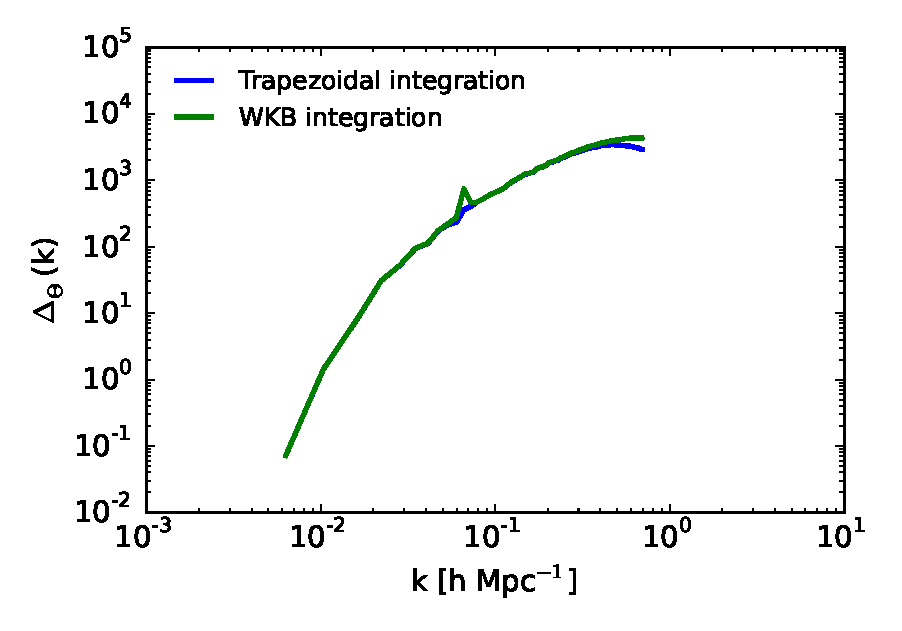
\includegraphics[width=\textwidth]{Figures/wkb_v_0.eps}
%     \caption{}\label{fig:wkb_v_0}
%   \end{subfigure}
%   \begin{subfigure}[t]{0.45\textwidth}
%     \centering
%     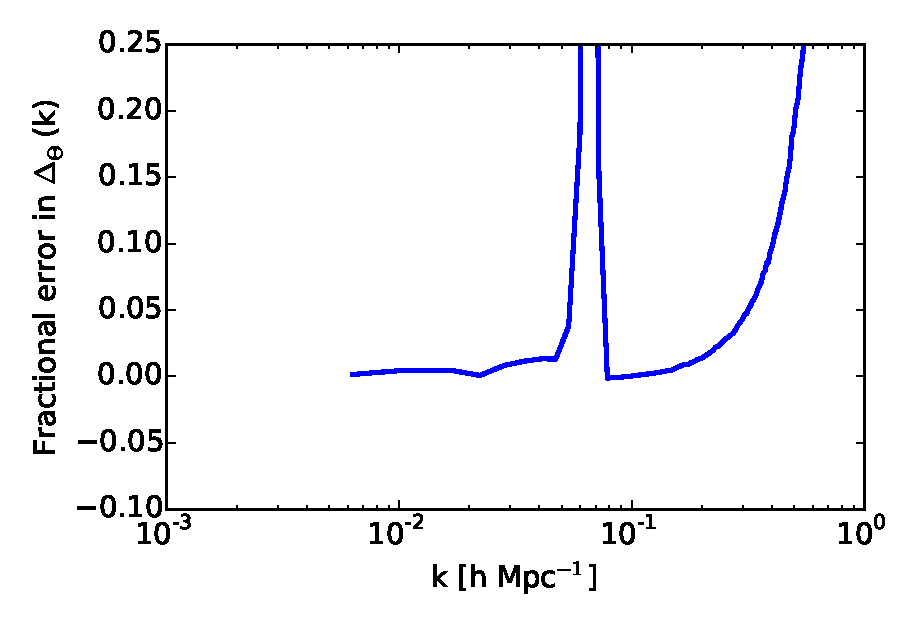
\includegraphics[width=\textwidth]{Figures/wkb_v_0_error.eps}
%     \caption{}\label{fig:wkb_v_0_error}
%   \end{subfigure}
%   \caption{A comparison of the trapezoidal and WKB integration
%     methods, specifically for the velocity divergence power of cold
%     dark matter.  In figure \ref{fig:wkb_v_0}, the integration results
%   are compared, while in figure \ref{fig:wkb_v_0_error} the fractional
% error of the WKB method compared to the trapezoidal method is shown.}\label{fig:wkb_v}
% \end{figure*}


% In Figure \ref{fig:wkb_v}, we compare the results of the
% trapezoidal and WKB integration method for the
% reconstruction of the CDM velocity divergence power, a
% case when the integrand is slowly varying and WKB integration is not
% required.  Figure \ref{fig:wkb_v} shows that while this WKB integration
% appears to be overly sensitive to some variations in the integrand, 
% causing the spike at $k=0.07$ h Mpc$^{-1}$, overall the
% method reproduces the integral with less than 25\% error up until
% $k=0.5$ h Mpc$^{-1}$. DOESNT SEEM LIKE FAR ENOUGH - EVERYTHING ELSE
% GOES UNTIL K=1.  WILL NEED TO LOOK AT HOW TO FIX THIS TO WORK AT
% HIGHER REDSHIFTS AD

%\begin{wrapfigure}{l}{0.5\linewidth}
\begin{figure*}[h!]
  \centering
    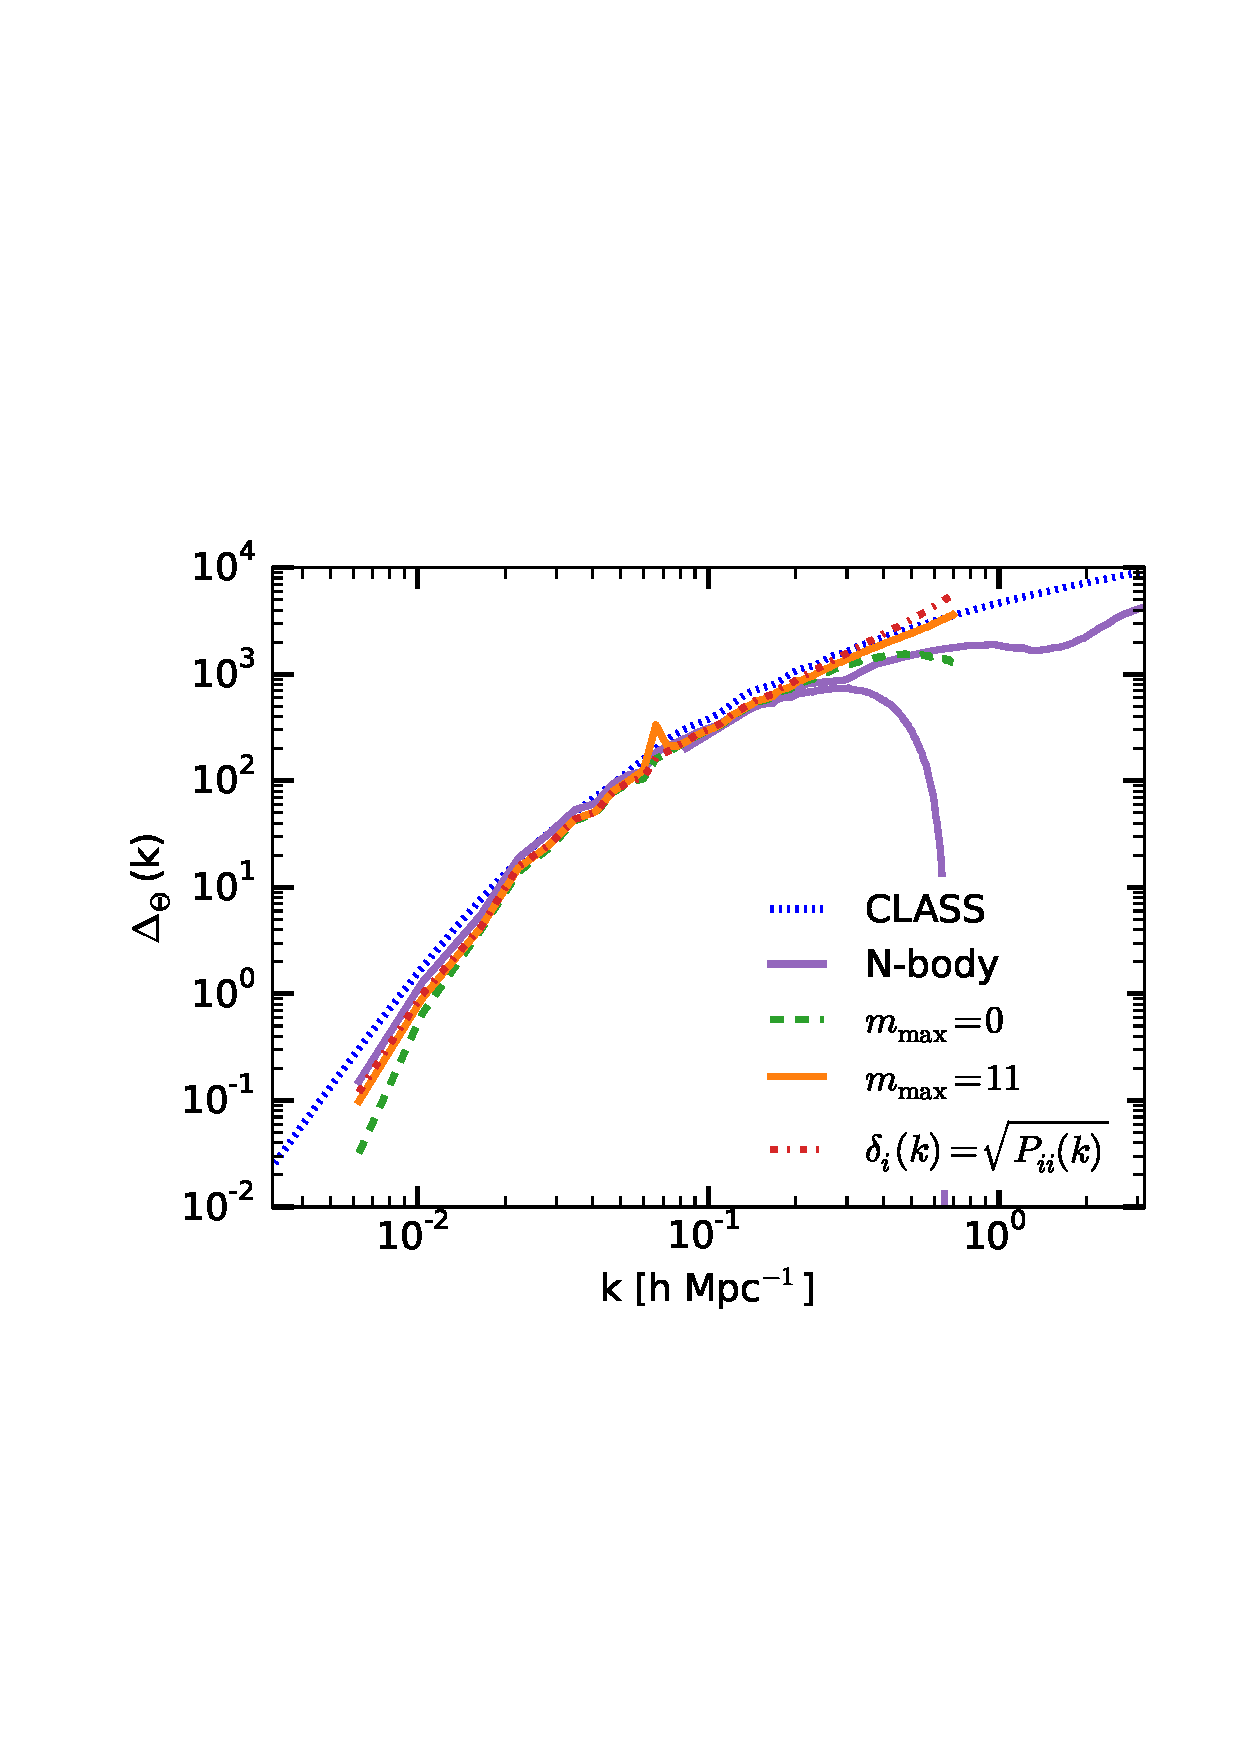
\includegraphics[width=0.495\textwidth]{Figures/vel_cdm_0.pdf}
    \caption{The semi-linear CDM velocity divergence
      power spectrum at $z=0$ along with 
      power spectra from the simulation (solid purple) and
      CLASS (dotted blue). The semi-linear power spectrum is calculated with only the primary
eigenmode from the decomposition of the cross-correlation matrix
(dashed green), with 12 modes (solid orange), and under the assumption
that the gravitational potential remains in phase over time
(dot-dashed red).  The velocity divergence spectra from two
    simulations are included for comparison, but only the simulation
    at smaller wavenumbers was used in the semi-linear method (see
    Section \ref{sec:Results}).  
    The semi-linear method 
    provides similar results to linear theory.  Including
    additional modes in the calculation increases the semi-linear
    power; however the
    numerical power is decreased on small scales compared to linear
    theory. 
    %We
  %also note that the power calculated when the changing gravitational
  %phase is ignored provides the highest power, and increasing the
  %number of modes in the semi-linear calculation drives the
  %semi-linear power towards the power calculated when the potential is
%assumed to have a constant phase.  These results indicate that the
%non-linear gravitational potential and its changing phase do not
%explain the reduced CDM velocity power on small scales.
}
    \label{fig:vel_cdm_rec}
\end{figure*}
%\end{wrapfigure}

Figure \ref{fig:vel_cdm_rec} shows the CDM
velocity divergence power spectra from CLASS, the simulation,
and the semi-linear method.  The results are similar to those for the
CDM density power.   Again, we see that
the semi-linear method does not improve significantly on the linear
results, and that the semi-linear results obtained with twelve eigenmodes
agree well with those obtained when the phase of the
gravitational potential is ignored. Interestingly, we see that even
though the N-body CDM velocity divergence spectrum is reduced
from linear theory on small scales, adding additional modes to the
semi-linear calculation increases the power on small scales, suggesting that
including 
the non-linear gravitational potential and accounting for the phase of
the gravitational potential do not to explain this departure
from linearity.

\begin{figure*}[h!]
  \centering
  \subfloat[$\sum m_\nu = 0.2$ eV\label{fig:vel_nu0p2_rec}]{
    \includegraphics[width=0.495\textwidth]{Figures/vel_nu0p2_0_pres.pdf}}
  \subfloat[$\sum m_\nu = 0.1$ eV\label{fig:vel_nu0p05_rec}]{
    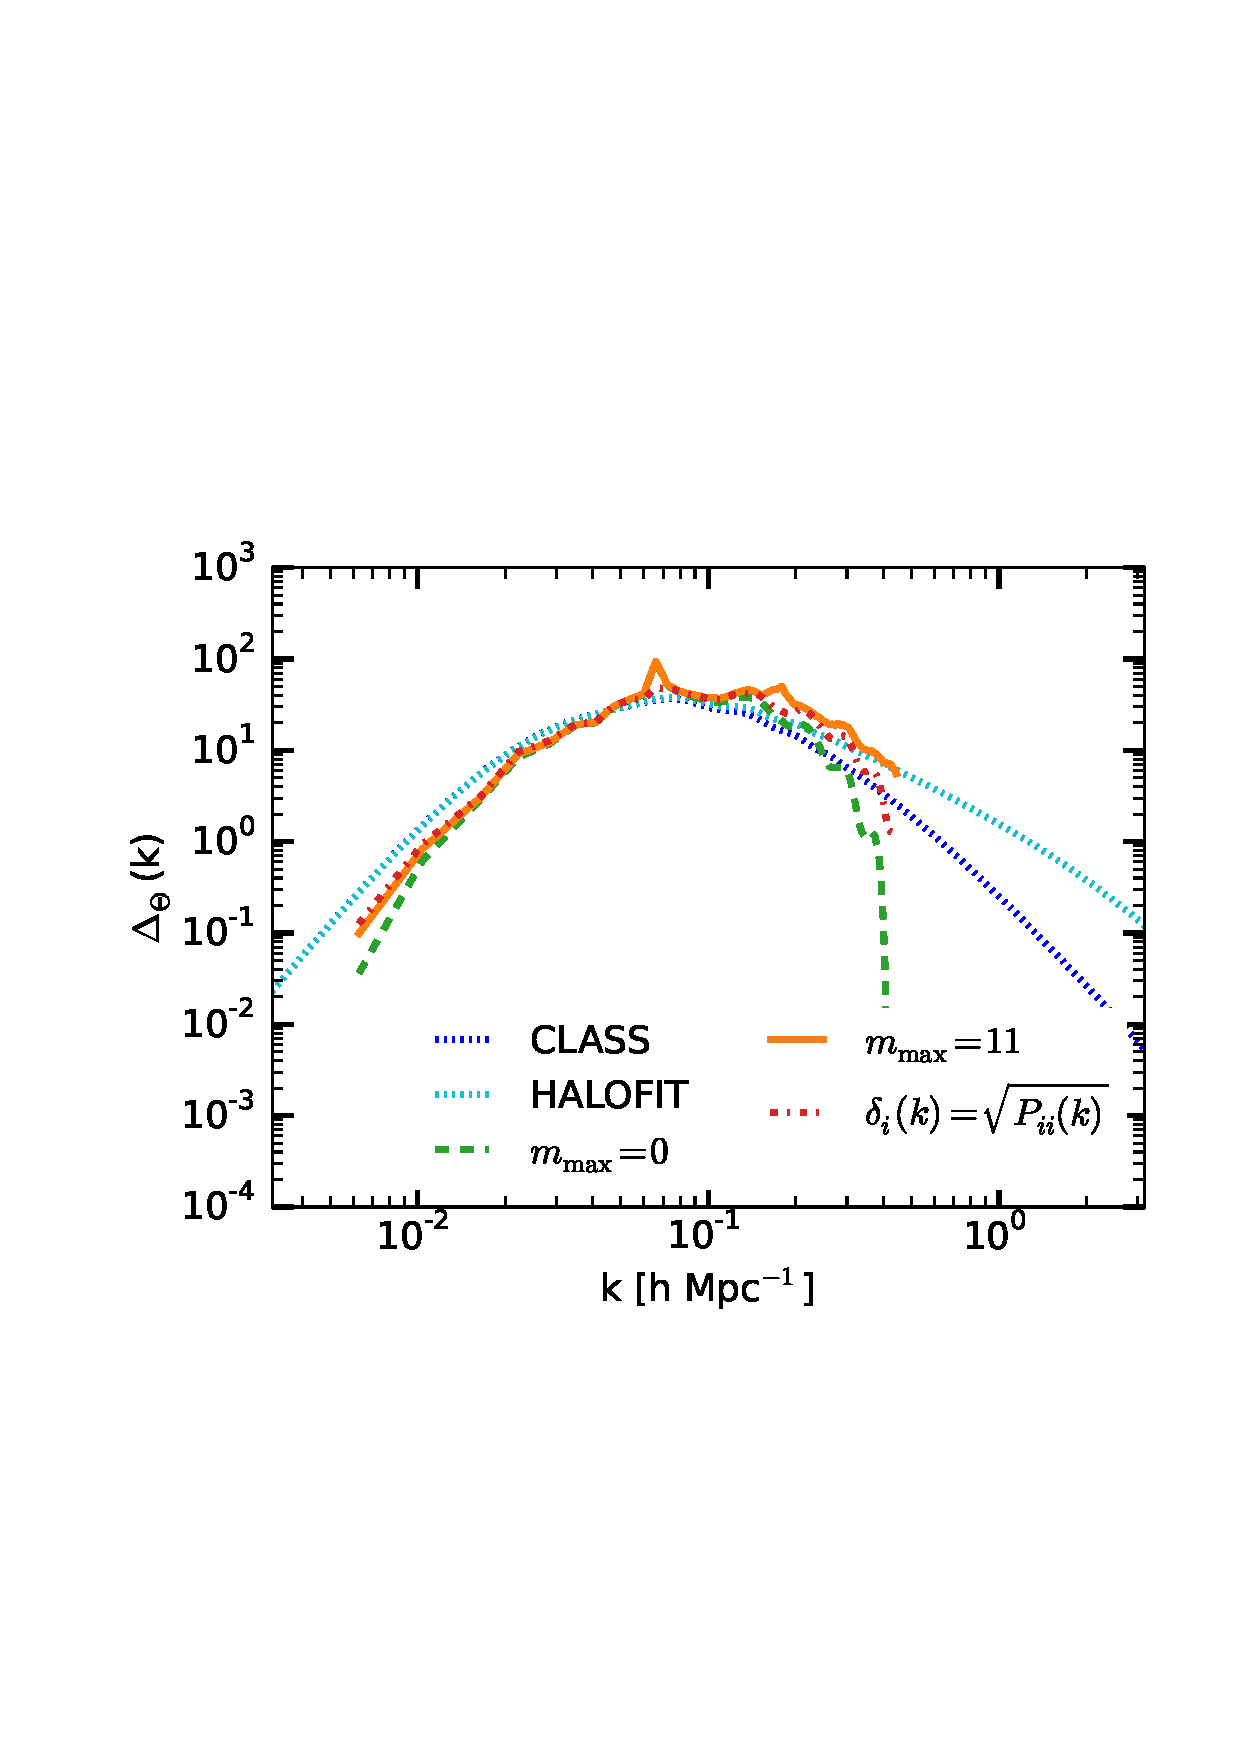
\includegraphics[width=0.495\textwidth]{Figures/vel_nu0p1_0.pdf}}
  \caption{The semi-linear neutrino velocity divergence power
      spectrum at $z=0$ for
     $\textstyle\sum m_\nu = 0.2$ eV (\ref{fig:vel_nu0p2_rec}) and $\textstyle\sum
     m_\nu = 0.1$ eV (\ref{fig:vel_nu0p05_rec}) along with the
     velocity  divergence
      power spectrum from CLASS (dotted blue), \halofit (dotted teal) and the N-body
      simulation (solid purple).  The semi-linear power spectrum is
      shown when only the primary mode of the
      cross-correlation matrix is included (dashed green), 
      when 12 modes are included (solid orange), and when the
      changing phase of the gravitational potential is ignored
      (dot-dashed red).  The numerical spectrum is not shown in Figure
      \ref{fig:vel_nu0p05_rec} as no simulation with $\textstyle\sum
      m_\nu = 0.1$ eV was performed.  
      The semi-linear method provides
      an improvement on linear theory, and traces the \halofit and
      numerical spectra closely.  
      %We see that when many modes are
      %included in the semi-linear method, the results are very similar
    %to those when the change in the gravitational phase is ignored.
}
    \label{fig:vel_nu_rec}
\end{figure*}

In Figure \ref{fig:vel_nu_rec}, the neutrino velocity divergence power
is shown 
for $\sum m_\nu = 0.2$ eV (Figure \ref{fig:vel_nu0p2_rec})
and $\sum m_\nu = 0.1$ eV (Figure \ref{fig:vel_nu0p05_rec}). 
Here,
we see that the semi-linear results are a significant correction to
linear theory and agree well with both the numerical and
\halofit power spectra.  
%This is understandable as both
%operate under the premise of a linear neutrino response to a
%non-linear gravitational potential. 
Again, we note that when all modes are
included, the results agree with those obtained
when changes in the gravitational potential phase are ignored.

\section{ Including Non-linearities in the Fluid Equations}
\label{sec:Nonlinear}
A possible improvement to this semi-linear approach 
is the inclusion of non-linear terms in the fluid equations. 
% New stuff
While this seems a natural direction to pursue, 
%at first
%glance it appears difficult to include non-linearities in the
%semi-linear approach as 
non-linear terms 
containing both $\delta_\nu$ and $\delta_c$ complicate the
integration of the fluid equations to calculate neutrino perturbations.  However,
considering that neutrino density perturbations are much smaller
than CDM density perturbations, it is possible to include
these non-linear terms through an iterative approach.
%If we first take these cross terms
%to be zero and calculate the neutrino density response,
%$\delta_\nu^0$, we can then use $\delta_\nu^0$ to calculate the cross
%terms.  
%The neutrino density response when
%these cross terms are included in the fluid equations,
%$\delta_\nu^1$, can then be calculated by a subsequent integration.  
%This process can be repeated until the results
%converge.  
In this section, we investigate this technique; %and apply it to
%include some non-linearities in the fluid equations; 
however, we leave
a rigorous treatment of the non-linearities to future work. 


THIS NEEDS TO BE REWRITTEN 

%Recall from
%Section \ref{sec:Theory} that we linearized the fluid
%equations by dropping all terms non-linear
%in the perturbations $\delta$ and $\mathbf{u}$.  
If we repeat the
derivation of the comoving fluid equations 
in Section \ref{sec:Theory} but do not linearize the fluid
equations, we can consider the effects of higher order perturbations to
 the CDM and neutrino density and velocity fluctuations.
%Recall as well our
%discussion that assuming that the fluids of interest are
%incompressible has the same results as linearizing the fluid
%equations.  For example, take the Euler equation in its full form
%(before the assumptions of a linear or incompressible fluid):
%\begin{equation}
 % 
%\end{equation}
We start with the full
compressible fluid equations in the Newtonian gauge before
conversion to comoving coordinates, Equations \eqref{eqn:continuity} and
\eqref{eqn:euler}, reproduced here for convenience:
\begin{equation} \label{eqn:contintuitytwo}
  \frac{ \partial \rho } {\partial t} + \nabla \cdot ( \rho \mathbf{v}
  ) = 0 
\end{equation}
and
\begin{equation}\label{eqn:eulertwo}
  \frac{ \partial \rho \mathbf{v} }{ \partial t} + ( \mathbf{v} \cdot
  \nabla ) (\rho \mathbf{v} ) + \nabla P_{T} = 0 \;.
\end{equation}
By differentiating Equation \eqref{eqn:contintuitytwo} with respect to
$t$ and taking the divergence of Equation \eqref{eqn:eulertwo} we
obtain, after some manipulation, the single equation:
\begin{equation}\label{eqn:nonlinear}
  \frac{ \partial^2 \rho }{\partial t^2} - \nabla \cdot ( (\mathbf{v}
  \cdot \nabla) \rho \mathbf{v} ) = \nabla^2 P - \nabla (\rho \nabla \Phi)\;,
\end{equation}
where $P$ is the pressure that is not due to
gravity. 
%
%WHY DO WE ONLY KEEP SOME SECOND ORDER TERMS AND NOT ALL OF THEM
After converting to comoving coordinates and linearizing Equation
\eqref{eqn:nonlinear} with respect to the variable $\mathbf{u}$ only,
we obtain the equation:
\begin{equation}\label{eqn:nonlinear2} 
  \ddot{\delta_i} -
  \frac{a^2}{
    \widebar{\rho_i}} \nabla^2P = a^2 \nabla( (1+\delta_i) \nabla (
  \phi_c ) ) = \frac{3}{2} H^2(\tau) \nabla( (1+\delta_i)\nabla\phi_c) \;,
\end{equation}
where a coordinate transformation from $t$ to $\tau$ has been made such that
$\frac{d}{d\tau}= a^2\frac{d}{dt}$, $\dot{f}$ is the derivative of $f$ with respect to $\tau$, and
$H(\tau) = \frac{1}{a} \frac{da}{d\tau}$.
Equation \eqref{eqn:nonlinear} is linearized
with respect to $\mathbf{u}$ but not $\delta$ as we expect
the density perturbation to be more significant than the
velocity
perturbation, as seen throughout this analysis (\eg Figures
\ref{fig:density} and \ref{fig:vel}).

Equation \eqref{eqn:nonlinear2} differs from Equation
\eqref{eqn:densitycontrast2}, the linearized equation for the density
perturbation, by only the right hand side. 
Therefore, to obtain the density power
spectra from Equation \eqref{eqn:nonlinear2}, we can use the same Green's functions as
in Section \ref{sec:Density}.  The change in the right hand side is
accounted for by defining a new set of vectors, $z_i$, analogous
to the $w$-vectors so that:
\begin{align*}
  <(\nabla& ((1 + \delta_i(\tau)) \nabla \delta_c(\tau)) (\nabla
  ((1+\delta_i(\tau')) \nabla \delta_c(\tau')))^*> \\
&= \sum_m
  z_i^m(\tau) z_i^m(\tau')\;, \numberthis
\end{align*}
where we have suppressed the $k$ dependence of $\delta$ and $z$.  
Note that we require a set of $z$-vectors for both neutrinos ($i=\nu$) and
CDM ($i=c$), and that we need the neutrino density
field to define $z_\nu$.
We can write the density power as:
\begin{equation}\label{eqn:nonlinear3}
  P_{i,z}(k,\tau) = \sum_m \bigg| \int_{-\infty}^\tau d\tau' G_i(\tau,\tau')
  \frac{3}{2} H^2(\tau') z_i^m(k, \tau') \bigg|^2\;,
\end{equation} 
where the subscript $z$ indicates that this is the power driven by the
$z$-vectors, and $G_i(\tau, \tau')$ are the Green's functions from Section
\ref{sec:Density}:
\begin{equation}
  G_c(\tau,\tau') = \tau-\tau'
\end{equation}
and
\begin{equation}
  G_\nu(\tau,\tau') = \sin( \tau-\tau')\;.
\end{equation}

When calculating the CDM density power spectrum from
Equation \eqref{eqn:nonlinear3}, we obtain the driving term
$\nabla((1+\delta_c)\nabla\delta_c)$ 
from numerical simulations.  
Similarly, we can calculate the $z_\nu$-vectors using density
fields from the simulation including neutrinos.
 %However, we can also use the iterative process mentioned above
However, as our goal is to replace
N-body simulations of neutrinos with a semi-linear method, we would
like to omit any dependence on the neutrino density fields from
simulations.  This can be done by generating %the linear 
%by generating
neutrino density fields
at the desired redshifts
using the initial conditions generator for CUBEP$^3$M. If we normalize
the density
fields
to the neutrino power spectra driven by the $w$-vectors 
from Section \ref{sec:Density}, 
they can be used to calculate the
$z$-vectors and the neutrino response to the $\nabla ((1+\delta_\nu)
\nabla \phi_c)$ driving term.  This
process can then be repeated using the newly obtained neutrino
power spectra to normalize the neutrino density fields.  We can
reiterate this procedure until the results converge.  In the results presented
below, only four iterations of this method were used.


%RESULTS HERE
%\subsection{ Reconstruction with Nonlinear Driving}

\begin{figure*}[h!]
  \centering
  \subfloat[CDM\label{fig:nlcdm}]{
    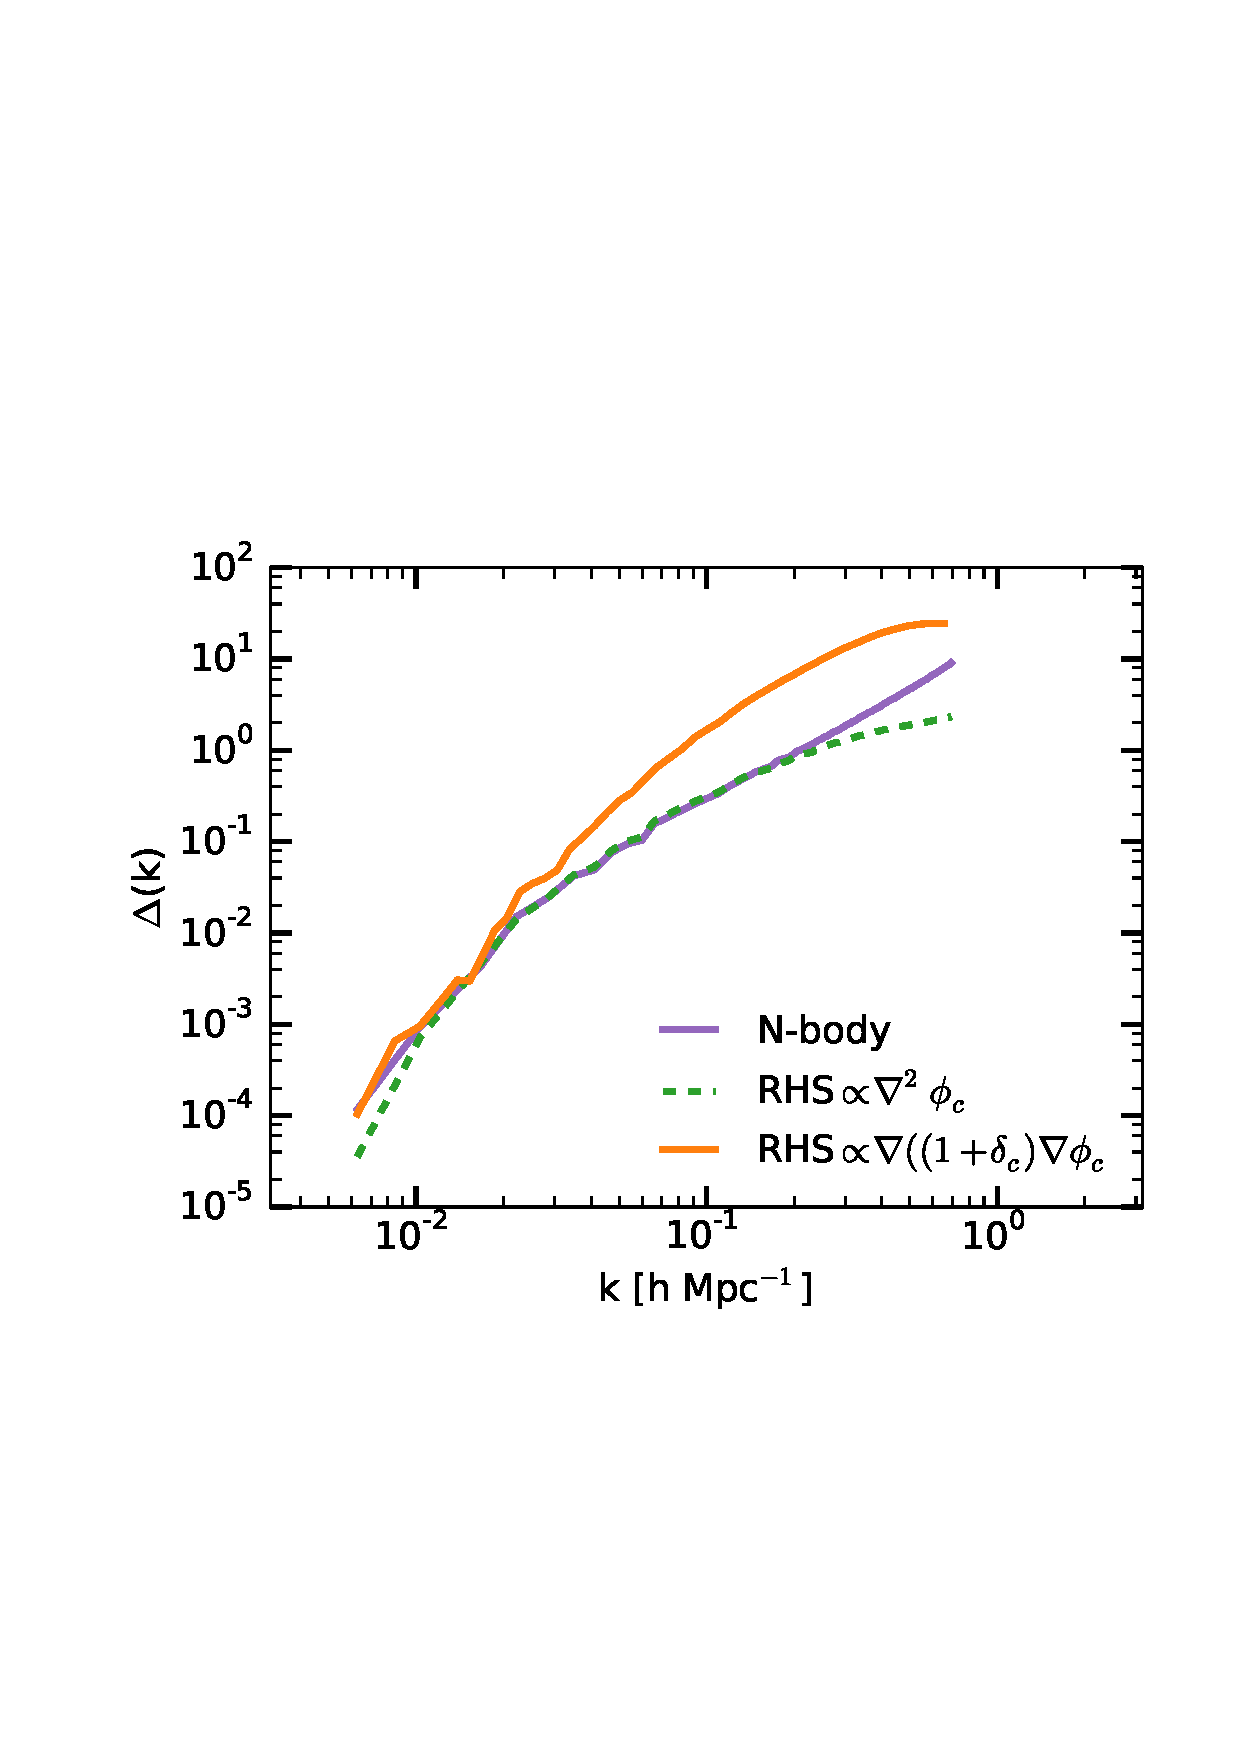
\includegraphics[width=0.495\textwidth]{Figures/density_cdm_nl_0.pdf}}
  \subfloat[Neutrinos\label{fig:nlnu}]{
    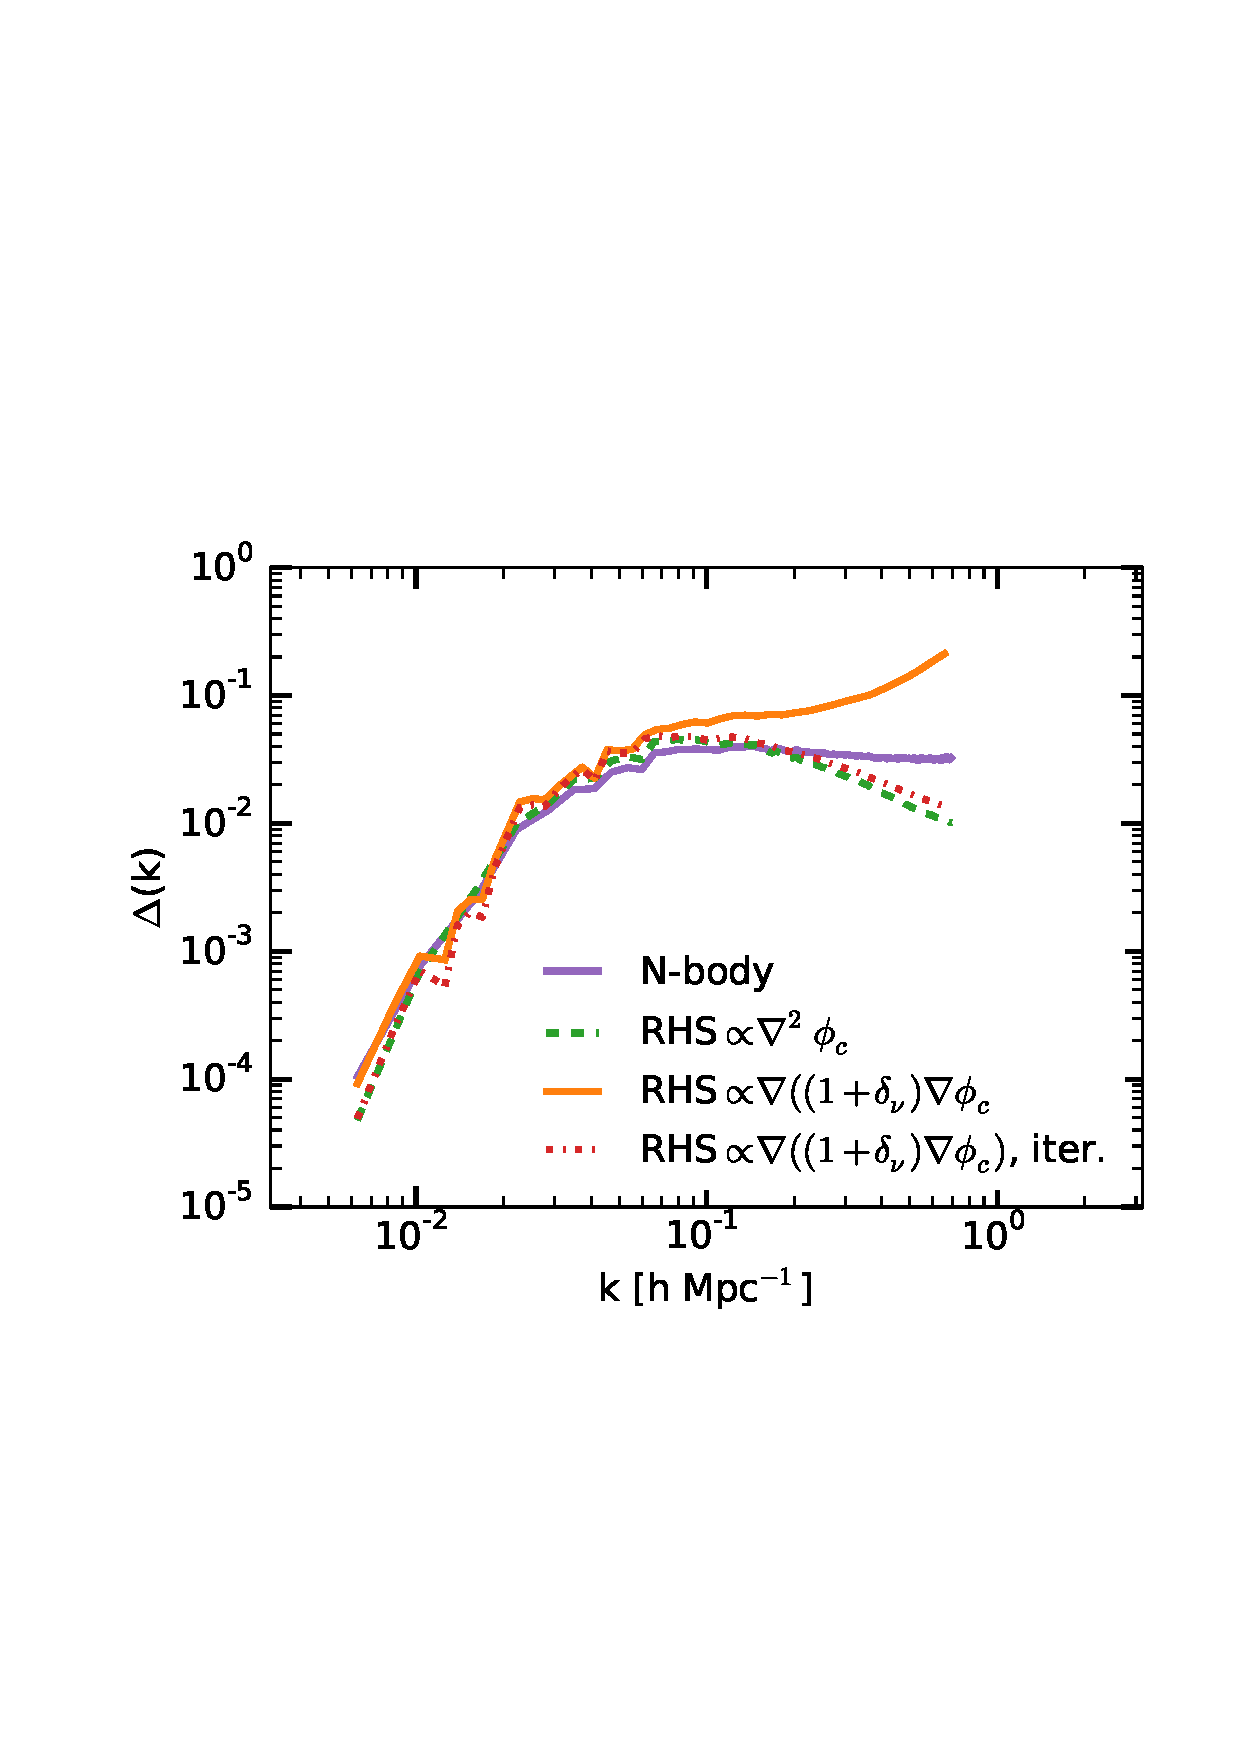
\includegraphics[width=0.495\textwidth]{Figures/density_nu_nl_0.pdf}}
  \caption{The CDM (\ref{fig:nlcdm}) and neutrino
    (\ref{fig:nlnu}) density power spectra calculated from the
    $z$-vectors (solid orange), which are
    computed from the cross-correlation coefficients of $\nabla
    ((1+\delta_i) \nabla \phi)$ ($i=c,\nu$ for CDM and neutrinos
    respectively), at $z=0$ alongside the power spectra from the 
    numerical simulations 
    (solid purple) and from the semi-linear calculation using 
    the $w$-vectors (dashed
    green).  In
    Figure \ref{fig:nlnu}, the response to the $z$-vectors
    calculated using the iterative method to 4th order (dot-dashed red) is
    also shown. The power calculated from the $z$-vectors
    overestimates the numerical density power for both
    species. 
    %We also note that the iterative method used to calculate
    %the neutrino spectrum is very slow to converge to the
    %$\nabla(1+\delta_\nu)\nabla\phi$ response calculated using numerical
    %density fields. 
}\label{fig:nl}
\end{figure*}

In Figure \ref{fig:nl}, we show the density power spectra of CDM and
neutrinos calculated from Equation \eqref{eqn:nonlinear3}.
%The non-linear driving response is found using the density
%fields from the N-body simulation with neutrinos to compute the
%non-linear driving term.  However, as our ultimate goal is to replace
%N-body simulations of neutrinos with this method, we would like to be
%able to calculate the response of neutrinos to this non-linear term
%without requiring the density field of neutrinos from N-body
%simulations.  This can be done by generating a neutrino density field
%using the initial conditions generator for CUBEP$^3$M at the desired
%redshift normalized to the neutrino power spectrum found using our
%semi-linear method with the driving term proportional to $\nabla^2
%\phi_c$.  This density field can then be used to calculate the
%non-linear driving term, and the neutrino response to this term.  This
%method can be repeated iteratively until the results converge.  
%We
%attempted four iterations of this method, producing the fourth order
%result in Figure \ref{fig:nlnu}.  
As can be seen from Figure \ref{fig:nlnu}, the neutrino density power
spectrum calculated at 4th order in the iterative method has a
 higher power than the 0th order results (\ie the results
calculated from the $w$-vectors), but convergence towards the power
calculated using the $z$-vectors from the numerical simulation is slow.  
%Part of this problem may
%be the low resolution of the density fields at high $k$, and a larger simulation may be
%required to fully investigate the use of this iterative method. 
A likely reason for the slow convergence is that the
neutrino density fields are generated with random phases and therefore
we expect little to
no cross-correlation between the neutrino and
CDM density fields on small scales in the iterative method.  In contrast, when using the
N-body fields, we expect a significant cross-correlation
between the neutrino and CDM density fields as 
neutrinos are most likely to cluster where CDM is
significantly clustered.  A more realistic treatment of the neutrino
density fields is therefore one in which we assume that the
neutrino and CDM densities 
are in phase, so that we can write:
\begin{equation}
  \delta_\nu(\mathbf{k},t) = \sqrt{ \frac{ P_\nu(k,t)}{P_c(k,t)} } \delta_c(\mathbf{k},t)\;.
\end{equation}
We will investigate this method in future work.

Figure \ref{fig:nl} shows that for both CDM and 
neutrinos, the density power response to the $z$-vectors is
significantly larger than the N-body power spectrum even at very low
$k$.  This is likely due to terms omitted from the fluid equations,
including higher order terms in the velocity perturbation.
%SHOULD TALK MORE ABOUT THIS.
Another possibility is that the pressure experienced by CDM
and neutrinos is underestimated at late times and on small
scales.  Indeed, in our analysis we treat CDM as a
pressureless fluid; however, when CDM clusters this
assumption is no longer valid; in order for halos to be in static
equilibrium, the clustered CDM must be experiencing an outward
pressure to balance the inward gravitational pressure.  An outward
pressure would resist structure formation and therefore reduce the
power on small scales, driving the power spectrum in the correct direction.
%, causing the semi-linear power spectrum to be
%corrected in the correct direction.
%In order to
%investigate the effects that such a pressure would have, we added a
%dark matter sound speed with a linear dependence on the scalefactor,
%$a$, to take into account the fact that the pressure experienced by
%the dark matter increases at late times when the dark matter has
%clustered on small scales. ADD THIS TO THE PLOT.  As you can see, the
%addition of this sound speed reduces the dark matter power at large
%scales.  
To investigate the effects of the pressure more
thoroughly, the CDM pressure can be
calculated from numerical simulations and incorporated into the fluid equations.
We will pursue these possible additions to the non-linear fluid equations in future work.

%\section{Accuracy Improvements}
%\label{sec:Improvements}
%Up until now, the equations that we have used have included
%significant approximations; for example, we have are currently using
%the linearized fluid equations and have dropped advection (?) terms
%from the Euler equation.  There are a number of ways to both check the
%validity of these approximations and improve upon them, which will be
%detailed in this section. 

%\subsection{Continuity Equation}
%\label{sec:Continuity}

%CONFUSED ABOUT EXACTLY WHAT WE DID HERE. I THINK WE USED THE EULER
%EQUATION? BUT I THOUGHT WE HAD USED THE CONTINUITY BECAUSE FEWER
%APPROXIMATIONS.  LOOK AT LATER.

%All mentions seem to use the euler equation here.  
%\begin{equation}
%\begin{array}{rcl}
%  \dot{ v } &=& - \nabla \phi_c \\[1em]
%  v &=& \nabla \int dt \phi_c \\[1em]
%<v v^*> &=& k^2 < \phi_c \phi_c^* >  \\[1em]
%            &=& \frac{1}{k^2} < \delta_c \delta^*_c >
%\end{array}
%\end{equation}
%So we integrated the w-vectors with no Green's function and then
%compared it to the velocity power from the cubep3m code??
%What we actually did was integrate the continuity equation, getting
%the grad(1+delta)u from the code. 
%However, I dont know if we actually got the (1+delta)u or just u ->
%will need to look at this later to see.  If we just used the u then I
%dont know how much we have to gain from this exercise.  

%One method of determining exactly which approximations have important
%effects on the results is to use the same methods used to calculate,
%for example, the neutrino power spectrum, in other calculations that
%require only some and not all of the approximations and
%discretization used in the calculation of the power spectrum.  In
%order to pursue this, we examined the continuity equation, equation
%\ref{eqn:continuity}.  If we start again with the full form of the
%equation, before any approximations but in comoving coordinates we
%have:
%\begin{equation}
%\label{eqn:continuity6}
%  \dot{delta} + \frac{1}{a} \nabla( (1+\delta ) \mathbf{u} )
%\end{equation}
%Now, if we let $\mathbf{q} = \nabla (1+delta) \mathbf{u}$ be a measure of the
%momentum, then we can write:
%\begin{equation}
%\label{eqn:continuity7}
%\delta(t) = - \int_{0}^{t} dt \frac{1}{a} \mathbf{q} 
%\end{equation}
%This form of the continuity equation does not rely on the assumptions
%of linearity, or of incompressible flows.  Therefore, by studying this
%equation we can determine the effect of outputting results from the
%simulations at discrete redshifts, and confirm the wavenumbers for
%which the discretization reproduces exact results. 

%To do this we used the N-body simulations to print out the $<q(t)
%q^*(t')>$ unequal-time power spectra at the same redshifts as the CDM
%unequal-time power spectra, and then calculated the $w_q$ vectors for
%the $q$-power, analogously to the $w$ vectors for the dark matter
%power spectrum.  Once the $w_q$ vectors are calculated, the $q$ power
%spectrum can be written in terms of the $w_q$ vectors as:
%\begin{equation}
 % \label{eqn:wqvectors}
 % P_q(t,t',k) = <q(t,k)q(t',k)> = \sum_m <w_q(t,k) w_q^*(t',k) > 
%\end{equation}
%So that we may write the dark matter power spectrum in terms of the
%$w_q$ vectors using equation \ref{eqn:continuity7}:
%\begin{equation}
 % \label{eqn:continuity8}
 % P(t,k) = <\delta(t,k) \delta^*(t,k) > = \sum_m \bigg | \int_0^t dt'
 % \frac{1}{a(t')} w_q(t',k) \bigg|^2
%\end{equation}
%By comparing the reconstructed dark matter power spectrum in equation
%\ref{eqn:continuity8} to the actual dark matter power spectrum from
%the N-body code, we are then able to assess the effects of
%only retaining output from the code at discrete redshifts.

%RESULTS HERE
%DISCUSSION HERE


%\section{Discussion}
%\label{sec:Discussion}

%Discussion discussion discussion discussion


\section{Conclusions and Future Work}
\label{sec:Conclusions}

We have presented a
semi-linear treatment of neutrinos in a $\Lambda$CDM
universe that includes the
fully non-linear behaviour of CDM from N-body
simulations.  While this method succeeds at
improving upon linear theory, it does not accurately
reproduce the N-body neutrino power spectrum for
$k\gsim0.2$ h Mpc$^{-1}$.  The
numerical neutrino velocity divergence power, however, is well-characterized by
this semi-linear method.  The relative success of the application of
the semi-linear method to the 
neutrino velocity divergence power compared to the
neutrino density power may be due to the fact that the velocity
divergence tends to be better characterized by linear theory than the density.
Using unequal-time cross-correlation
coefficients to retain phase information on the gravitational potential
from the N-body simulation allows us to discuss the effects of
 subordinate modes on the power spectra; however, when many modes are included
 the results converge to those
obtained when the phase of the gravitational potential is assumed to
be constant with redshift. 
This method applied to CDM 
provides little improvement on linear theory, as is expected: A fluid approximation of CDM is
obviously inappropriate when the CDM density field is non-linear.  

%We note that the results for the
%neutrinos agree very well with those obtained when we scale the linear
%CLASS neutrino spectra by the ratio of the HALOFIT and CLASS matter
%power spectra.  This is not surprising, as both of these methods
%essentially treat a linear neutrino fluid in a non-linear
%gravitational potential.  
The inaccuracy of this method compared to the
N-body neutrino power spectrum on small scales 
indicates that a linear
fluid treatment of neutrinos on these scales may not be appropriate.
In future work, we hope to improve upon these results by
including higher order perturbations in the neutrino fluid equations.
To provide a more conclusive
analysis of this method, we must also look at
running high resolution simulations to successfully model the
power spectra on smaller scales.  We can match this with the
semi-linear method by including more modes in our decomposition of the
unequal-time cross correlation matrix, thereby testing the applicability of
this method to modelling non-linearities on much smaller scales than
those 
discussed in this work. 
%This semi-linear method can also be modified to
%treat any fluid in a $\Lambda$CDM background and therefore can be
%applied to areas beyond the study of neutrinos, such as the study of
%fluid models of 
%dark energy.
%In the future we should also run a simulation with a lower neutrino
%mass to see how the errors scale with mass
%At high wavenumbers, the effects of neutrinos on the CDM power
%spectrum become important.  We plan to investigate these effects
%by evolving the fluid approximation of the neutrinos simultaneously
%with the N-body simulation, performing the integrations in this report
%at every time-step and incorporating the neutrino contribution to the
%total gravitational potential. 
%** means we
%cant use the mode by mode analysis so same as what yacine does - not
%worth it unless we improve on the non-linear result


The semi-linear method proposed in this work allows for the study of
non-linear neutrino behaviour without relying on
N-body simulations of neutrinos.  As a result, it is very rapid and simple to
implement.
% even though it incorporates the neutrino response to the 
%full non-linear gravitational potential sourced by CDM.  
Since it is easy to include various fluid properties in 
the analytic treatment of neutrinos, 
%is easy to adapt to incorporate various
%neutrino properties, 
this semi-linear method is well-suited to the investigation of
the effects these properties have on the neutrino power spectra. 
For example, very low mass neutrinos or neutrinos with a time-varying
mass are extremely difficult to simulate numerically but are easily
modelled using this semi-linear method.
%Although this method fails to reproduce the
%fully non-linear N-body neutrino power spectrum, it does improve on the purely linear method
%and therefore should be considered as an alternative to a fully linear
%approach for studies that do not lend themselves well to a
%particle treatment of neutrinos, for example, studies of very low-mass
%neutrinos, or of neutrinos with a time-varying mass.  
Studies of
non-linear neutrino behaviour are important for predicting and
interpreting the results of future searches for 
direct detections of relic neutrinos, such as the
\ptolemy experiment.  If we understand non-linear neutrino behaviour
and its dependence on cosmology,
studies of cosmic neutrinos stand to provide insight not only into
neutrinos but also into the early universe they probe. 



%This
%method is also easily applied to any fluid in a cosmology where
%the gravitational potential is dominated by CDM,
%and therefore may be of use 

%The semi-linear method presented here is easily adapted to any fluid
%in a $\Lambda CDM$ universe, and therefore may be 
%TALK ABOU
% other fluids eg. logotropic dark matter
% origin of vorticity

\section*{ Acknowledgments }
%\acknowledgments
I would like to thank Derek Inman
and J.D. Emberson for their support with
the CUBEP$^3$M simulations.
Computations were performed on the GPC supercomputer at the SciNet HPC
Consortium.  SciNet is funded by: the Canada Foundation for
Innovation under the auspices of Compute Canada; the Government of
Ontario; Ontario Research Fund - Research Excellence; and the
University of Toronto.

\medskip
\bibliography{paper}{}

%1003.0942 -> good information on why we can represent neutrinos as
%fluids, and why we do it

\appendix

% \section{Relating the Neutrino and Photon
%   Temperatures}\label{app:AppA}
% We can relate the cosmic neutrino background and CMB
% temperatures as follows.
% Before decoupling, neutrinos and photons were in
% thermal equilibrium.  After decoupling, both the photon and neutrino
% temperatures decreased due to the expansion of the universe: $T
% \propto a^{-1}$. However, in addition to this decrease, the temperature of the
% photon distribution was increased by the annihilation of positrons
% and electrons. As this occurred after decoupling, the neutrino
% temperature was unaffected by this period of annihilation.  
% %As the
% %neutrinos had already decoupled from the photons, they were unaffected
% %by this occurrence.  NEED TO REFERENCE THIS SHIT 
% This lead to a difference in the neutrino and
% photon temperature, which may be obtained 
%  by comparing the effective number of degrees of
% freedom contributed by relativistic species in thermal equilibrium
% with photons before and after annihilation.  The
% effective number of relativistic degrees of freedom for particles in
% thermal equilibrium with photons is given by \citep{baumann3}: 
% % This is from
% % http://www.damtp.cam.ac.uk/user/db275/Cosmology/Chapter3.pdf but we
% % may need to find a different source to cite.
% \begin{equation}\label{eqn:dof}
%   g_*^{th}(T) = \sum_{i=b} g_i + \frac{7}{8} \sum_{i=f} g_i \;,
% \end{equation}
% where the species labels $b$ and $f$ refer to bosons and fermions
% respectively and $g$ is the number of degrees of freedom, $g_b=2$ and
% $g_f=4$.
% %gf = 4 because we count the antiparticles * spin states
%  Using Equation \eqref{eqn:dof} we find:
% \begin{equation}
%   \frac{ g_*^{th}(T\gg T_{ann})}{g_*^{th}(T\ll T_{ann})} = \frac{ 2 + 4
%     (\frac{7}{8})}{ 2 } = \frac{11}{4} \;,
% \end{equation}
% where $T_{ann}$ is the temperature at which the heating of the photons
% due to the positron-electron annihilation occurs.  
% %Note that each species
% %has two degrees of freedom for the two spin states, and that before
% %annihilation we include photons, electrons and positrons in the
% %calculation of the effective number of relativistic degrees of
% %freedom.  
% During positron-electron annihilation, the photon
% temperature varies as $ T_\gamma \propto (g_*^{th})^{-1/3} a^{-1} $, so that after
% the heating of photons due to positron-electron annihilation the ratio
% of the cosmic photon and neutrino background temperatures is given by:
% \begin{equation}
%   \frac{T_\nu}{T_\gamma} = \bigg( \frac{g_*^{th}(  T \gg T_{ann} )}{ g_*^{th}(T
%     \ll T_{ann})}   \bigg)^{1/3} =\bigg(\frac{4}{11}\bigg)^{1/3} \;.
% \end{equation}


% \section{Neutrino Velocity Dispersion}\label{app:AppB}
% Recall the definition of the velocity dispersion:
% \begin{align*}\label{eqn:veldisp2}
%   \sigma_v^2 &= \frac{1}{a^2 m^2 } < q >^2\\
%   &= \frac{1}{a^2\, m^2} \frac{ \int_0^\infty q^2 dq q^2 f_0(q) }{
%       \int_0^\infty q^2 dq f_0(q) } \;.\numberthis
% \end{align*}
% Recall from Section \ref{sec:NuFluid} that neutrinos obey the
% relativistic Fermi-Dirac distribution, Equation \eqref{eqn:fermidirac} as they are relativistic at the
% time of decoupling.  Also recall that after decoupling, the neutrino
% temperature varies only due to the expansion of the universe, so that
% $aT$ remains constant and we can use the relation $a(t)T_\nu(t) = a_0T_{\nu,0}$,
% where the subscript $0$ denotes values today.  
% Using Equation \eqref{eqn:fermidirac}, 
% the integral in the denominator can be evaluated as follows:
% \begin{align*}\label{eqn:veldisp3}
%   \int_0^\infty dq q^4 f_0(q) &= \int_0^\infty dq q^4
%                                   \frac{1}{\me^{q/T_0} + 1} \\
%   &= T_{nu,0}^5 \int_0^\infty dx \frac{ x^4 }{\me^x +1 } \\
%   &= T_{nu,0}^5 \frac{45}{2} \zeta (5) \;,\numberthis
% \end{align*}
% where the substitution $x=q/T_0$ was made and $\zeta(x)$ is the
% Riemann zeta function.  The integral in the numerator evaluates to:
% \begin{align*}\label{eqn:veldisp4}
%   \int_0^{\infty} dq q^2 f_0(q) &= \int_0^\infty dq q^2
%                                     \frac{1}{\me^{q/T_0}+1}\\
%  &= T_{\nu,0}^3 \int_0^\infty dx \frac{x^2}{\me^x+1}\\
%  &= T_{\nu,0}^3 \frac{3}{2} \zeta(3) \;.\numberthis
% \end{align*}
% Substituting these integrals into Equation \eqref{eqn:veldisp2} we find:
% \begin{equation}\label{eqn:veldisp52}
%   \sigma_v^2(t) = \frac{1}{a^2(t)\,m^2_\nu} 15 \frac{ \zeta(5)
%   }{\zeta(3) }  T_{\nu,0}^2 \;.
% \end{equation}
% This is the relation used in the derivation of the neutrino sound
% speed in Section \ref{sec:NuFluid}.

\end{document}
